% Options for packages loaded elsewhere
% Options for packages loaded elsewhere
\PassOptionsToPackage{unicode}{hyperref}
\PassOptionsToPackage{hyphens}{url}
\PassOptionsToPackage{dvipsnames,svgnames,x11names}{xcolor}
%
\documentclass[
  english,
  letterpaper,
  DIV=11,
  numbers=noendperiod]{scrreprt}
\usepackage{xcolor}
\usepackage{amsmath,amssymb}
\setcounter{secnumdepth}{5}
\usepackage{iftex}
\ifPDFTeX
  \usepackage[T1]{fontenc}
  \usepackage[utf8]{inputenc}
  \usepackage{textcomp} % provide euro and other symbols
\else % if luatex or xetex
  \usepackage{unicode-math} % this also loads fontspec
  \defaultfontfeatures{Scale=MatchLowercase}
  \defaultfontfeatures[\rmfamily]{Ligatures=TeX,Scale=1}
\fi
\usepackage{lmodern}
\ifPDFTeX\else
  % xetex/luatex font selection
\fi
% Use upquote if available, for straight quotes in verbatim environments
\IfFileExists{upquote.sty}{\usepackage{upquote}}{}
\IfFileExists{microtype.sty}{% use microtype if available
  \usepackage[]{microtype}
  \UseMicrotypeSet[protrusion]{basicmath} % disable protrusion for tt fonts
}{}
\makeatletter
\@ifundefined{KOMAClassName}{% if non-KOMA class
  \IfFileExists{parskip.sty}{%
    \usepackage{parskip}
  }{% else
    \setlength{\parindent}{0pt}
    \setlength{\parskip}{6pt plus 2pt minus 1pt}}
}{% if KOMA class
  \KOMAoptions{parskip=half}}
\makeatother
% Make \paragraph and \subparagraph free-standing
\makeatletter
\ifx\paragraph\undefined\else
  \let\oldparagraph\paragraph
  \renewcommand{\paragraph}{
    \@ifstar
      \xxxParagraphStar
      \xxxParagraphNoStar
  }
  \newcommand{\xxxParagraphStar}[1]{\oldparagraph*{#1}\mbox{}}
  \newcommand{\xxxParagraphNoStar}[1]{\oldparagraph{#1}\mbox{}}
\fi
\ifx\subparagraph\undefined\else
  \let\oldsubparagraph\subparagraph
  \renewcommand{\subparagraph}{
    \@ifstar
      \xxxSubParagraphStar
      \xxxSubParagraphNoStar
  }
  \newcommand{\xxxSubParagraphStar}[1]{\oldsubparagraph*{#1}\mbox{}}
  \newcommand{\xxxSubParagraphNoStar}[1]{\oldsubparagraph{#1}\mbox{}}
\fi
\makeatother

\usepackage{color}
\usepackage{fancyvrb}
\newcommand{\VerbBar}{|}
\newcommand{\VERB}{\Verb[commandchars=\\\{\}]}
\DefineVerbatimEnvironment{Highlighting}{Verbatim}{commandchars=\\\{\}}
% Add ',fontsize=\small' for more characters per line
\usepackage{framed}
\definecolor{shadecolor}{RGB}{241,243,245}
\newenvironment{Shaded}{\begin{snugshade}}{\end{snugshade}}
\newcommand{\AlertTok}[1]{\textcolor[rgb]{0.68,0.00,0.00}{#1}}
\newcommand{\AnnotationTok}[1]{\textcolor[rgb]{0.37,0.37,0.37}{#1}}
\newcommand{\AttributeTok}[1]{\textcolor[rgb]{0.40,0.45,0.13}{#1}}
\newcommand{\BaseNTok}[1]{\textcolor[rgb]{0.68,0.00,0.00}{#1}}
\newcommand{\BuiltInTok}[1]{\textcolor[rgb]{0.00,0.23,0.31}{#1}}
\newcommand{\CharTok}[1]{\textcolor[rgb]{0.13,0.47,0.30}{#1}}
\newcommand{\CommentTok}[1]{\textcolor[rgb]{0.37,0.37,0.37}{#1}}
\newcommand{\CommentVarTok}[1]{\textcolor[rgb]{0.37,0.37,0.37}{\textit{#1}}}
\newcommand{\ConstantTok}[1]{\textcolor[rgb]{0.56,0.35,0.01}{#1}}
\newcommand{\ControlFlowTok}[1]{\textcolor[rgb]{0.00,0.23,0.31}{\textbf{#1}}}
\newcommand{\DataTypeTok}[1]{\textcolor[rgb]{0.68,0.00,0.00}{#1}}
\newcommand{\DecValTok}[1]{\textcolor[rgb]{0.68,0.00,0.00}{#1}}
\newcommand{\DocumentationTok}[1]{\textcolor[rgb]{0.37,0.37,0.37}{\textit{#1}}}
\newcommand{\ErrorTok}[1]{\textcolor[rgb]{0.68,0.00,0.00}{#1}}
\newcommand{\ExtensionTok}[1]{\textcolor[rgb]{0.00,0.23,0.31}{#1}}
\newcommand{\FloatTok}[1]{\textcolor[rgb]{0.68,0.00,0.00}{#1}}
\newcommand{\FunctionTok}[1]{\textcolor[rgb]{0.28,0.35,0.67}{#1}}
\newcommand{\ImportTok}[1]{\textcolor[rgb]{0.00,0.46,0.62}{#1}}
\newcommand{\InformationTok}[1]{\textcolor[rgb]{0.37,0.37,0.37}{#1}}
\newcommand{\KeywordTok}[1]{\textcolor[rgb]{0.00,0.23,0.31}{\textbf{#1}}}
\newcommand{\NormalTok}[1]{\textcolor[rgb]{0.00,0.23,0.31}{#1}}
\newcommand{\OperatorTok}[1]{\textcolor[rgb]{0.37,0.37,0.37}{#1}}
\newcommand{\OtherTok}[1]{\textcolor[rgb]{0.00,0.23,0.31}{#1}}
\newcommand{\PreprocessorTok}[1]{\textcolor[rgb]{0.68,0.00,0.00}{#1}}
\newcommand{\RegionMarkerTok}[1]{\textcolor[rgb]{0.00,0.23,0.31}{#1}}
\newcommand{\SpecialCharTok}[1]{\textcolor[rgb]{0.37,0.37,0.37}{#1}}
\newcommand{\SpecialStringTok}[1]{\textcolor[rgb]{0.13,0.47,0.30}{#1}}
\newcommand{\StringTok}[1]{\textcolor[rgb]{0.13,0.47,0.30}{#1}}
\newcommand{\VariableTok}[1]{\textcolor[rgb]{0.07,0.07,0.07}{#1}}
\newcommand{\VerbatimStringTok}[1]{\textcolor[rgb]{0.13,0.47,0.30}{#1}}
\newcommand{\WarningTok}[1]{\textcolor[rgb]{0.37,0.37,0.37}{\textit{#1}}}

\usepackage{longtable,booktabs,array}
\usepackage{calc} % for calculating minipage widths
% Correct order of tables after \paragraph or \subparagraph
\usepackage{etoolbox}
\makeatletter
\patchcmd\longtable{\par}{\if@noskipsec\mbox{}\fi\par}{}{}
\makeatother
% Allow footnotes in longtable head/foot
\IfFileExists{footnotehyper.sty}{\usepackage{footnotehyper}}{\usepackage{footnote}}
\makesavenoteenv{longtable}
\usepackage{graphicx}
\makeatletter
\newsavebox\pandoc@box
\newcommand*\pandocbounded[1]{% scales image to fit in text height/width
  \sbox\pandoc@box{#1}%
  \Gscale@div\@tempa{\textheight}{\dimexpr\ht\pandoc@box+\dp\pandoc@box\relax}%
  \Gscale@div\@tempb{\linewidth}{\wd\pandoc@box}%
  \ifdim\@tempb\p@<\@tempa\p@\let\@tempa\@tempb\fi% select the smaller of both
  \ifdim\@tempa\p@<\p@\scalebox{\@tempa}{\usebox\pandoc@box}%
  \else\usebox{\pandoc@box}%
  \fi%
}
% Set default figure placement to htbp
\def\fps@figure{htbp}
\makeatother



\ifLuaTeX
\usepackage[bidi=basic]{babel}
\else
\usepackage[bidi=default]{babel}
\fi
% get rid of language-specific shorthands (see #6817):
\let\LanguageShortHands\languageshorthands
\def\languageshorthands#1{}
\ifLuaTeX
  \usepackage[english]{selnolig} % disable illegal ligatures
\fi


\setlength{\emergencystretch}{3em} % prevent overfull lines

\providecommand{\tightlist}{%
  \setlength{\itemsep}{0pt}\setlength{\parskip}{0pt}}



 


\KOMAoption{captions}{tableheading}
\makeatletter
\@ifpackageloaded{bookmark}{}{\usepackage{bookmark}}
\makeatother
\makeatletter
\@ifpackageloaded{caption}{}{\usepackage{caption}}
\AtBeginDocument{%
\ifdefined\contentsname
  \renewcommand*\contentsname{Table of contents}
\else
  \newcommand\contentsname{Table of contents}
\fi
\ifdefined\listfigurename
  \renewcommand*\listfigurename{List of Figures}
\else
  \newcommand\listfigurename{List of Figures}
\fi
\ifdefined\listtablename
  \renewcommand*\listtablename{List of Tables}
\else
  \newcommand\listtablename{List of Tables}
\fi
\ifdefined\figurename
  \renewcommand*\figurename{Figure}
\else
  \newcommand\figurename{Figure}
\fi
\ifdefined\tablename
  \renewcommand*\tablename{Table}
\else
  \newcommand\tablename{Table}
\fi
}
\@ifpackageloaded{float}{}{\usepackage{float}}
\floatstyle{ruled}
\@ifundefined{c@chapter}{\newfloat{codelisting}{h}{lop}}{\newfloat{codelisting}{h}{lop}[chapter]}
\floatname{codelisting}{Listing}
\newcommand*\listoflistings{\listof{codelisting}{List of Listings}}
\makeatother
\makeatletter
\makeatother
\makeatletter
\@ifpackageloaded{caption}{}{\usepackage{caption}}
\@ifpackageloaded{subcaption}{}{\usepackage{subcaption}}
\makeatother
\usepackage{bookmark}
\IfFileExists{xurl.sty}{\usepackage{xurl}}{} % add URL line breaks if available
\urlstyle{same}
\hypersetup{
  pdftitle={Predictive Modeling of Residential Property Prices in Pierce County},
  pdfauthor={Edberto Moura Lima; Gerta Hajrullahi; Helga Deutschmann; Mira Radakovic},
  pdflang={en},
  colorlinks=true,
  linkcolor={blue},
  filecolor={Maroon},
  citecolor={Blue},
  urlcolor={Blue},
  pdfcreator={LaTeX via pandoc}}


\title{Predictive Modeling of Residential Property Prices in Pierce
County}
\author{Edberto Moura Lima \and Gerta Hajrullahi \and Helga
Deutschmann \and Mira Radakovic}
\date{2026-05-11}
\begin{document}
\maketitle

\renewcommand*\contentsname{Table of contents}
{
\hypersetup{linkcolor=}
\setcounter{tocdepth}{2}
\tableofcontents
}

\bookmarksetup{startatroot}

\chapter*{Preface}\label{preface}
\addcontentsline{toc}{chapter}{Preface}

\markboth{Preface}{Preface}

This documentation presents the project proposal and development
progress for the Predictive Modeling of Residential Property Prices in
Pierce County, developed as part of the Solution Engineering course at
FHTW.

The project aims to build a robust machine learning pipeline to estimate
housing prices by integrating diverse data sources from the Pierce
County Assessor-Treasurer. This book serves as the central repository
for project objectives, data descriptions, organizational structure, and
development plans.

\section*{Project Team}\label{project-team}
\addcontentsline{toc}{section}{Project Team}

\markright{Project Team}

\begin{itemize}
\tightlist
\item
  \textbf{Mira Radakovic} (Project Leader)
\item
  \textbf{Edberto Moura Lima} (Data Analyst)
\item
  \textbf{Gerta Hajrullahi} (Data Analyst)
\item
  \textbf{Helga Deutschmann} (Data Analyst)
\end{itemize}

\section*{Document Status}\label{document-status}
\addcontentsline{toc}{section}{Document Status}

\markright{Document Status}

This version corresponds to the \textbf{Project Proposal (Report 1)}.

\begin{itemize}
\tightlist
\item[$\boxtimes$]
  Project Objectives (Qualitative \& Quantitative)
\item[$\boxtimes$]
  Data Source Description \& Dictionary
\item[$\boxtimes$]
  Project Organization \& Task Allocation
\item[$\boxtimes$]
  Development Plan \& Workflow
\item[$\boxtimes$]
  Gantt Schedule \& Milestones
\end{itemize}

\bookmarksetup{startatroot}

\chapter{Project Objective}\label{project-objective}

\section{Background \& Motivation}\label{background-motivation}

Estimating house prices is a classic regression problem with clear
real-world importance. Housing markets are influenced by many
interconnected factors, including property characteristics, location,
neighborhood effects, and market trends over time. Because nearby
properties often share similar values and market conditions change
continuously, house-price prediction provides an excellent example for
applying the complete data-science workflow covered in this course.

For this project, the publicly available Assessor--Treasurer data from
Pierce County is used as the main data source. The dataset contains
detailed and realistic information about properties, transactions, and
assessments across multiple linked tables, offering a large-scale and
practical environment for data exploration, pre-processing, feature
engineering, and predictive modeling.

\section{Project Goal}\label{project-goal}

Develop a machine learning system capable of predicting residential
property prices using structural, spatial, economic, and neighborhood
characteristics.

\section{Qualitative Objectives}\label{qualitative-objectives}

\begin{enumerate}
\def\labelenumi{\arabic{enumi}.}
\item
  Build a clean housing dataset for Pierce County.
\item
  Explore which factors influence house prices.
\item
  Engineer predictive variables from property and spatial data.
\item
  Compare traditional statistical and machine learning approaches.
\item
  Deploy a simple Shiny app for interactive price estimation.
\item
  Allow non-technical users to test predictions using custom property
  inputs.
\item
  Create visual outputs that support decision-making.
\end{enumerate}

\section{Quantitative Objectives}\label{quantitative-objectives}

\begin{longtable}[]{@{}
  >{\raggedright\arraybackslash}p{(\linewidth - 4\tabcolsep) * \real{0.4074}}
  >{\raggedright\arraybackslash}p{(\linewidth - 4\tabcolsep) * \real{0.2963}}
  >{\raggedright\arraybackslash}p{(\linewidth - 4\tabcolsep) * \real{0.2963}}@{}}
\toprule\noalign{}
\begin{minipage}[b]{\linewidth}\raggedright
Objective
\end{minipage} & \begin{minipage}[b]{\linewidth}\raggedright
Metric
\end{minipage} & \begin{minipage}[b]{\linewidth}\raggedright
Target
\end{minipage} \\
\midrule\noalign{}
\endhead
\bottomrule\noalign{}
\endlastfoot
\textbf{Model Accuracy} & Root Mean Square Error (RMSE) & 80\% within
15\% from actual price \\
\textbf{Explanatory Power} & Coefficient of Determination (R²) &
\textgreater{} 0.85 \\
\textbf{Model Diversity} & Algorithm Benchmarking & ≥ 4 distinct
algorithms \\
\textbf{Feature Richness} & Engineered Predictors & ≥ 20 model-ready
features \\
\textbf{App Performance} & Real-time Inference & Response time
\textless{} 3 seconds \\
\textbf{Data Integrity} & Table Integration & 100\% of selected source
tables joined \\
\end{longtable}

: Quantitative project success criteria and performance targets.
\{\#tbl-quantitative-objectives\}

\section{Deliverables \& Timeline}\label{deliverables-timeline}

\begin{itemize}
\tightlist
\item
  \textbf{21.05.2026}: Project Proposal Presentation
\item
  \textbf{06.06.2026}: Interim Results Presentation
\item
  \textbf{24.06.2026}: Final Results Presentation \& Project Report
  Submission
\item
  \textbf{24.06.2026}: Live demo of deployed model App
\end{itemize}

\bookmarksetup{startatroot}

\chapter{Data Source Description \& Data
Dictionary}\label{data-source-description-data-dictionary}

\section{Overview}\label{overview}

The Pierce County Assessor--Treasurer Data Mart is a comprehensive
relational database containing detailed property assessment, taxation,
appraisal, land-use, improvement, and sales transaction records
maintained by Pierce County, Washington. The dataset integrates
information from multiple administrative systems and organizes it into
interconnected tables linked primarily through the parcel identification
number, enabling consistent tracking of individual properties across
taxation, valuation, ownership, and structural characteristics.

The database includes information related to property accounts, land
attributes, building improvements, tax assessments, exemption
categories, sales history, and geographic identifiers. Together, these
tables provide a multidimensional representation of residential and
commercial properties and support both fiscal administration and
real-estate market analysis.

Here we provide a data dictionary with detailed descriptions of the
available tables, attributes, data types, and relationships that form
the foundation for exploratory data analysis, spatial analysis, and
predictive modeling of residential property prices in Pierce County.

\begin{center}\rule{0.5\linewidth}{0.5pt}\end{center}

\section{Relational Diagram}\label{relational-diagram}

The data mart uses a relational schema with the following structure:

\begin{figure}

\centering{

\pandocbounded{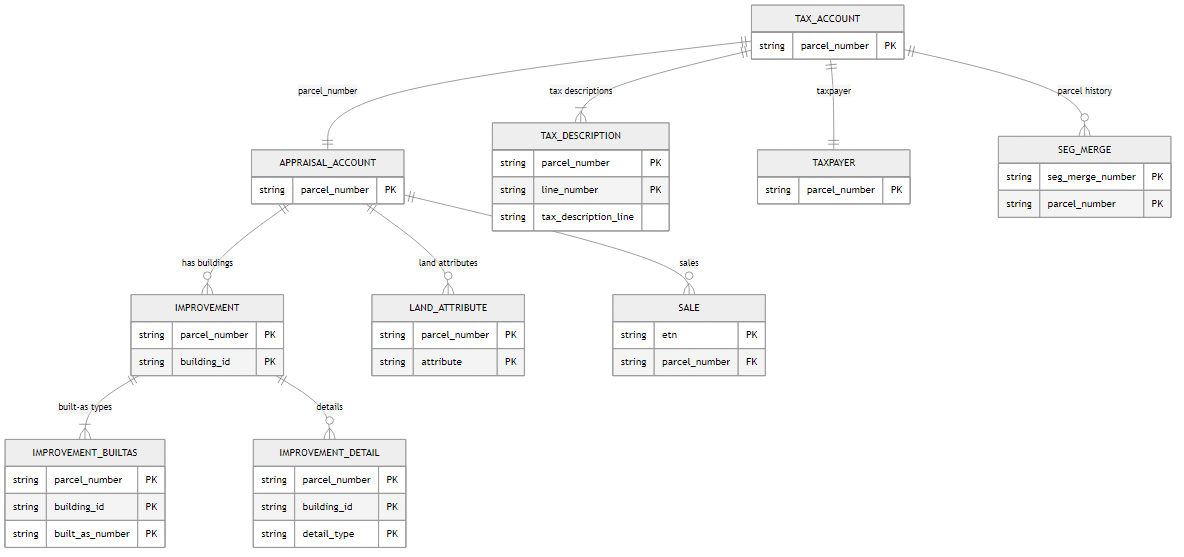
\includegraphics[keepaspectratio]{diagrams/er-diagram.png}}

}

\caption{\label{fig-pierce-er}Entity--relationship diagram of the Pierce
County data showing relationships among tax, appraisal, land,
improvement, taxpayer, and sales tables.}

\end{figure}%

\begin{center}\rule{0.5\linewidth}{0.5pt}\end{center}

\section{Table Definitions}\label{table-definitions}

\subsection{Tax Account}

Tracks current tax and assessment account information for each property.

\begin{longtable}[]{@{}
  >{\raggedright\arraybackslash}p{(\linewidth - 6\tabcolsep) * \real{0.2738}}
  >{\raggedright\arraybackslash}p{(\linewidth - 6\tabcolsep) * \real{0.1071}}
  >{\raggedright\arraybackslash}p{(\linewidth - 6\tabcolsep) * \real{0.1071}}
  >{\raggedright\arraybackslash}p{(\linewidth - 6\tabcolsep) * \real{0.5119}}@{}}
\caption{Pierce County data dictionary - field definitions and
descriptions for all tables.}\label{tbl-data-dictionary}\tabularnewline
\toprule\noalign{}
\begin{minipage}[b]{\linewidth}\raggedright
Field Name
\end{minipage} & \begin{minipage}[b]{\linewidth}\raggedright
Type
\end{minipage} & \begin{minipage}[b]{\linewidth}\raggedright
Size
\end{minipage} & \begin{minipage}[b]{\linewidth}\raggedright
Description
\end{minipage} \\
\midrule\noalign{}
\endfirsthead
\toprule\noalign{}
\begin{minipage}[b]{\linewidth}\raggedright
Field Name
\end{minipage} & \begin{minipage}[b]{\linewidth}\raggedright
Type
\end{minipage} & \begin{minipage}[b]{\linewidth}\raggedright
Size
\end{minipage} & \begin{minipage}[b]{\linewidth}\raggedright
Description
\end{minipage} \\
\midrule\noalign{}
\endhead
\bottomrule\noalign{}
\endlastfoot
\textbf{Parcel Number} & Text & 10 & Unique 10 digit number assigned to
each property \\
Account Type & Text & 5 & REAL - Real Property; STRUC - Structures; PERS
- Personal Property; MOBIL - Mobile Home \\
Property Type & Text & 5 & ASIMP - Administrative Seg Improvement; LNDIM
- Land and Improvements; MBLHM - Mobile Home; RRLEA - Railroad Leases;
SAPP - State Assessed Personal Property; SARP - State Assessed Real
Property; STRUC - Leased Land and/or Structure \\
Site Address & Text & 50 & Physical location address of the property.
May be different than mailing address. ``XXX'' indicates estimated
address using GIS \\
Use Code & Text & 5 & 4-digit numeric code for present highest and best
use of the property \\
Use Description & Text & 50 & Text description of the numeric use
code \\
Tax Year - Prior & Integer & & Tax year for which all prior year values
apply \\
Tax Code Area - Prior Year & Text & 10 & Code describing geographical
area and specific combination of taxing districts. Subject to annual
change \\
Exemption Type - Prior Year & Text & 40 & Type of exemption, if any,
applied to the property \\
Current Use Code - Prior Year & Text & 5 & AGRI - Agricultural; CT -
Current Use Timber; FORDG - Forest Designated; OPBRS - Open Space PBRS;
OPEN - Open Space \\
Land Value - Prior Year & Integer & & Total fair market value of land,
as determined by appraisal process \\
Improvement Value - Prior Year & Integer & & Total fair market value of
improvements (buildings, structures), as determined by appraisal
process \\
Total Market Value - Prior Year & Integer & & Total fair market value of
land and improvements, as determined by appraisal process \\
Taxable Value - Prior Year & Integer & & Market value of the property,
minus any exemptions granted \\
Tax Year - Current & Integer & & Tax year for which all current year
values apply \\
Tax Code Area - Current Year & Text & 10 & Code describing geographical
area and specific combination of taxing districts \\
Exemption Type - Current Year & Text & 40 & Type of exemption, if any,
applied to the property \\
Current Use Code - Current Year & Text & 5 & AGRI - Agricultural; CT -
Current Use Timber; FORDG - Forest Designated; OPBRS - Open Space PBRS;
OPEN - Open Space \\
Land Value - Current Year & Integer & & Total fair market value of land
for the parcel \\
Improvement Value - Current Year & Integer & & Total fair market value
of improvements (buildings, structures) for the parcel \\
Total Market Value - Current Year & Integer & & Total fair market value
of land and improvements for the parcel \\
Taxable Value - Current Year & Integer & & Market value of the property,
minus any exemptions granted \\
Range & Text & 10 & Range \\
Township & Text & 10 & Township \\
Section & Text & 20 & Section \\
Quarter Section & Text & 20 & Quarter \\
Subdivision Name & Text & 50 & Subdivision name \\
Located On Parcel & Text & 10 & Real property parcel number on which
this improvement-only parcel is located (Personal Property, Mobile
Homes, Leasehold Structures) \\
\end{longtable}

\subsection{Appraisal Account}

Detailed property appraisal data with characteristics and valuations.

\begin{longtable}[]{@{}
  >{\raggedright\arraybackslash}p{(\linewidth - 6\tabcolsep) * \real{0.2738}}
  >{\raggedright\arraybackslash}p{(\linewidth - 6\tabcolsep) * \real{0.1071}}
  >{\raggedright\arraybackslash}p{(\linewidth - 6\tabcolsep) * \real{0.1071}}
  >{\raggedright\arraybackslash}p{(\linewidth - 6\tabcolsep) * \real{0.5119}}@{}}
\toprule\noalign{}
\begin{minipage}[b]{\linewidth}\raggedright
Field Name
\end{minipage} & \begin{minipage}[b]{\linewidth}\raggedright
Type
\end{minipage} & \begin{minipage}[b]{\linewidth}\raggedright
Size
\end{minipage} & \begin{minipage}[b]{\linewidth}\raggedright
Description
\end{minipage} \\
\midrule\noalign{}
\endhead
\bottomrule\noalign{}
\endlastfoot
\textbf{Parcel Number} & Text & 10 & Unique 10 digit number assigned to
each property \\
Appraisal Account Type & Text & 15 & Com Condo, Com Leasehold, Com Multi
Unit, Commercial, Industrial, Mobile Home, Reference, Res Com Condo, Res
Leasehold, Residential, Trended Invest \\
Business Name & Text & 50 & Main business name on the parcel, or space
number for mobile/manufactured home in a park \\
Value Area ID & Text & 10 & Identifies the Physical Inspection cycle for
each parcel (PI1 to PI6) \\
Land Economic Area & Text & 30 & Also known as LEA, ties parcels to land
valuation models. For Commercial: identifies land use model by PI year.
For Residential: location code identifying appraisal area, sector and
subsector. For Res Com Condos: relates directly to account land value \\
Buildings & Integer & & Represents the number of improvements
(buildings) located on a parcel \\
Group Account Number & Text & 30 & Identifies and ties all parcels
qualifying as one economic unit (contiguous assessment). Also identifies
all parcels in a condominium project \\
Land Gross Acres & Decimal & 15.4 & Total acres that make up the
economic unit which could include multiple parcels \\
Land Net Acres & Decimal & 15.4 & Size of the individual parcel in
acres \\
Land Gross Square Feet & Decimal & 15.4 & Total square feet that make up
the economic unit which could include multiple parcels \\
Land Net Square Feet & Decimal & 15.4 & Size of the individual parcel in
square feet \\
Land Gross Front Feet & Decimal & 15.4 & For commercial parcels: front
feet of the site facing the arterial. For residential: front feet of the
lot facing the address side. For waterfront: effective waterfront length
of individual lot or combination of lots under single ownership \\
Land Width & Integer & & Residential Use Only. Equal to the Net
Effective Waterfront Front Feet of the individual parcel, or using Group
Account allocation method, then the sum of Net Effective Waterfront
Front Feet for the group \\
Land Depth & Integer & & Residential Use Only. Equal to the Net
Effective Depth of the individual waterfront parcel, or using Group
Account allocation method, then the sum of Net Effective Depths for the
waterfront group. Measured from the top of the bank (where bulkhead
begins) to the inland property line \\
Submerged Area Square Feet & Integer & & Area of a parcel that is
submerged. Not included in the Gross or Net Square Feet \\
Appraisal Date & Date & & Indicates the most recent date an appraiser
physically observed the property and/or made changes to the record \\
Waterfront Type & Text & 30 & Describes the type of waterfront the
property adjoins or has legal access to \\
View Quality & Text & 30 & Assigned to reflect the market appeal of the
overall view available from the dwelling or property \\
Utility Electric & Text & 30 & Identifies if power is installed,
available or is not available on the property \\
Utility Sewer & Text & 30 & Identifies if sewer/septic is installed,
available or not available if the property does not support an on site
sewage disposal system (no perc) \\
Utility Water & Text & 30 & Identifies if water is installed, available
or is not available \\
Street Type & Text & 30 & Identifies if the access street is paved or
unpaved. If blank, the parcel could be a reference parcel or a mobile
home assessed as personal property \\
Latitude & Decimal & 10.5 & The latitude of the parcel centroid. Some
parcels may not have latitude/longitude coordinates (building-only,
mineral rights and reference parcels, as well as others not represented
in the GIS system) \\
Longitude & Decimal & 10.5 & The longitude of the parcel centroid \\
\end{longtable}

\subsection{Improvement}

Detailed building improvement data linked to appraisal accounts.

\begin{longtable}[]{@{}
  >{\raggedright\arraybackslash}p{(\linewidth - 6\tabcolsep) * \real{0.2738}}
  >{\raggedright\arraybackslash}p{(\linewidth - 6\tabcolsep) * \real{0.1071}}
  >{\raggedright\arraybackslash}p{(\linewidth - 6\tabcolsep) * \real{0.1071}}
  >{\raggedright\arraybackslash}p{(\linewidth - 6\tabcolsep) * \real{0.5119}}@{}}
\toprule\noalign{}
\begin{minipage}[b]{\linewidth}\raggedright
Field Name
\end{minipage} & \begin{minipage}[b]{\linewidth}\raggedright
Type
\end{minipage} & \begin{minipage}[b]{\linewidth}\raggedright
Size
\end{minipage} & \begin{minipage}[b]{\linewidth}\raggedright
Description
\end{minipage} \\
\midrule\noalign{}
\endhead
\bottomrule\noalign{}
\endlastfoot
\textbf{Parcel Number} & Text & 10 & Unique 10 digit number assigned to
each property \\
\textbf{Building ID} & Text & 5 & Unique identifier for each improvement
record on a parcel. Not all improvements are on a separate record and
may not always be in sequence \\
Property Type & Text & 15 & Links buildings to proper cost and
depreciation tables. Options include: Commercial, Duplex, Industrial,
Mobile Home, Multiple Unit, Out Building, Residential, Townhouse,
Triplex \\
Neighborhood & Text & 10 & Represents boundaries for land subject to
similar social, environmental, economic and governmental forces.
Boundaries are typically located within a geographic area defined by
natural, man-made, or political boundaries. Residential Neighborhoods
and LEA's are the same. Commercial Neighborhoods define the location of
the property while Commercial LEA's define the use of the property \\
Neighborhood Extension & Text & 10 & Based on property type: Commercial
- represents the primary occupancy or use of the property. Residential -
not used, therefore they are set to zero. Mobile/Manufactured Homes -
based upon the underlying land ownership. All Mobile/Manufactured homes
located on land owned by the Mobile/Manufactured home owner are coded
with the Neighborhood Extension 0. Exception - Mobile/Manufactured homes
located within a park and owned by the park owner, will carry the same
Neighborhood Extension as the park. Mobile Homes in a park have a
neighborhood extension of: PL 1 (P = Park, L = Leased); P2, P3, P4,
etc \\
Square Feet & Integer & & Sum of the square feet for the `built as'
types identified for the building. Each building may have one or more
`built as' type (see IMPROVEMENT BUILTAS table), though usually only
one. The exceptions are `built as' \# 124 and 126 (Add on only Res \&
Com) or any type of Storage Tank, where it represents the count of those
`built as' as opposed to the sum of their square feet \\
Net Square Feet & Integer & & Used primarily to calculate income on
commercial properties, where it typically represents the sum of the net
rentable area(s). This number may be representative of one or more
buildings. If part of a Group Account, these buildings may be located on
more than one parcel. For Residential it is equal to the built as square
feet or zero (0) \\
\end{longtable}

\subsection{Improvement Built-As}

Detailed specifications for building construction styles and features.

\begin{longtable}[]{@{}
  >{\raggedright\arraybackslash}p{(\linewidth - 6\tabcolsep) * \real{0.2738}}
  >{\raggedright\arraybackslash}p{(\linewidth - 6\tabcolsep) * \real{0.1071}}
  >{\raggedright\arraybackslash}p{(\linewidth - 6\tabcolsep) * \real{0.1071}}
  >{\raggedright\arraybackslash}p{(\linewidth - 6\tabcolsep) * \real{0.5119}}@{}}
\toprule\noalign{}
\begin{minipage}[b]{\linewidth}\raggedright
Field Name
\end{minipage} & \begin{minipage}[b]{\linewidth}\raggedright
Type
\end{minipage} & \begin{minipage}[b]{\linewidth}\raggedright
Size
\end{minipage} & \begin{minipage}[b]{\linewidth}\raggedright
Description
\end{minipage} \\
\midrule\noalign{}
\endhead
\bottomrule\noalign{}
\endlastfoot
\textbf{Parcel Number} & Text & 10 & Unique 10 digit number assigned to
each property \\
\textbf{Building ID} & Text & 5 & Unique identifier for each improvement
record on a parcel \\
\textbf{Built-As Number} & Integer & & Unique number identifying each
Built-As on an improvement. Sequential number assigned by the system
starting with the largest Built-As being number 1 \\
Built-As ID & Integer & & Number associated with the description of the
purpose or style of construction of the building \\
Built-As Description & Text & 255 & Original purpose for and/or style of
construction of the building. The Built As is associated with the
Marshall and Swift cost and depreciation tables \\
Built-As Square Feet & Integer & & Sum of the square feet for the `built
as' types identified for the building. Each building may have one or
more `built as' type, though usually only one. The exceptions are `built
as' \# 124 and 126 (Add on only Res \& Com) or any type of Storage
Tank \\
HVAC & Integer & & Code associated with the predominant heating source
for the built-as structure \\
HVAC Description & Text & 30 & Text description associated with the
predominant heating source for the built-as structure (Forced Air,
Electric Baseboard, Steam, etc) \\
Exterior & Text & 25 & Predominant type of construction materials used
for the exterior siding on Residential Buildings \\
Interior & Text & 15 & Predominant type of materials used on the
interior walls (Sheetrock or Paneling). Collected for Residential and
Mobile Homes only \\
Stories & Decimal & 13.2 & Number of floors/building levels above grade.
Stories do not include attic or basement areas \\
Story Height & Integer & & Based on property type: Commercial -
determined by taking an average of the overall ceiling heights of all
floors for the Blt As. Residential - determined by the majority of the
story height for the first floor (main). Story height is automatically
rounded by the system (The system rounds up for .5 and higher and rounds
down for anything below .5) \\
Sprinkler Square Feet & Integer & & Total square footage covered by a
sprinkler system. Sprinkler SF does not always equal the built as square
footage \\
Roof Cover & Text & 20 & Material used for the roof (Composition
Shingles, Wood Shake, Concrete Tile, etc) \\
Bedrooms & Integer & & Number of bedrooms listed for a residential
property (Collected for informational purposes only) \\
Bathrooms & Decimal & 7.2 & Number of baths listed for a residential
property. The number is listed as a decimal, i.e.~2.75 = two full and
one three-quarter baths. A tub/sink/toilet combination (plus any
additional fixtures) is considered 1.0 bath. A shower/sink/toilet
combination (plus any additional fixtures) is 0.75 bath. A sink/toilet
combination is .5 bath \\
Units & Integer & & Number of separate units within the building. For
Commercial properties, Units may be combined to generate an income
approach for the economic unit on building one \\
Class Code & Text & 20 & Code for one of five basic cost groups by type
of framing (supporting beams and columns), walls, floors and roof
structures, and fireproofing. Typically Commercial Buildings \\
Class Description & Text & 50 & Text description for one of five basic
cost groups by type of framing (supporting beams and columns), walls,
floors and roof structures, and fireproofing. Typically Commercial
Buildings \\
Year Built & Integer & & Year the building was built, as stated by the
building permit or a historical record \\
Year Remodeled & Integer & & Year in which improvements are made to the
existing structure that extend the life of the structure \\
Adjusted Year Built & Integer & & If greater than the Year Built, it
indicates improvements have been made to the original property over and
above normal maintenance which would effectively reduce the age of the
building \\
Physical Age & Integer & & Tax year less the adjusted year built equals
the physical age of the built as \\
Built-As Length & Integer & & Length of the mobile/manufactured home \\
Built-As Width & Integer & & Width of the mobile/manufactured home \\
Mobile Home Model & Text & 50 & Model of the mobile/manufactured home \\
\end{longtable}

\subsection{Improvement Detail}

Additional specific improvement characteristics and features.

\begin{longtable}[]{@{}
  >{\raggedright\arraybackslash}p{(\linewidth - 6\tabcolsep) * \real{0.2738}}
  >{\raggedright\arraybackslash}p{(\linewidth - 6\tabcolsep) * \real{0.1071}}
  >{\raggedright\arraybackslash}p{(\linewidth - 6\tabcolsep) * \real{0.1071}}
  >{\raggedright\arraybackslash}p{(\linewidth - 6\tabcolsep) * \real{0.5119}}@{}}
\toprule\noalign{}
\begin{minipage}[b]{\linewidth}\raggedright
Field Name
\end{minipage} & \begin{minipage}[b]{\linewidth}\raggedright
Type
\end{minipage} & \begin{minipage}[b]{\linewidth}\raggedright
Size
\end{minipage} & \begin{minipage}[b]{\linewidth}\raggedright
Description
\end{minipage} \\
\midrule\noalign{}
\endhead
\bottomrule\noalign{}
\endlastfoot
\textbf{Parcel Number} & Text & 10 & Unique 10 digit number assigned to
each property \\
\textbf{Building ID} & Text & 5 & Unique identifier for each improvement
record on a parcel \\
\textbf{Detail Type} & Text & 10 & Category that specific improvement
characteristics are coded under. Options include: Add On, Appliance,
Balcony, Basement, Carport, Elevator, Fixture, Garage, Mezzanine, Porch,
Rough In, Storage. The Add On type allows the appraiser to assign a
quality different from the main structure for the characteristics within
this field \\
Detail Description & Text & 50 & Brief explanation of the improvement
characteristic (Fireplace, PreFab/Stoves, Laundry Facility, Type of
Porch (Cvrd Wd Deck), Type of Bath (Bath 2 Fixture)) \\
Units & Decimal & 15.4 & Component parts of the building
characteristics. The units indicate either the square footage of the
structure or a count of each component. Examples: Appliance, Allowance,
1 (count) or Porch, Open Slab, 337 (sf), or Fixture -- Bath 3 Fixtures
-- 2 (count) \\
\end{longtable}

\subsection{Land Attribute}

Land-specific attributes and characteristics affecting valuation.

\begin{longtable}[]{@{}
  >{\raggedright\arraybackslash}p{(\linewidth - 6\tabcolsep) * \real{0.2738}}
  >{\raggedright\arraybackslash}p{(\linewidth - 6\tabcolsep) * \real{0.1071}}
  >{\raggedright\arraybackslash}p{(\linewidth - 6\tabcolsep) * \real{0.1071}}
  >{\raggedright\arraybackslash}p{(\linewidth - 6\tabcolsep) * \real{0.5119}}@{}}
\toprule\noalign{}
\begin{minipage}[b]{\linewidth}\raggedright
Field Name
\end{minipage} & \begin{minipage}[b]{\linewidth}\raggedright
Type
\end{minipage} & \begin{minipage}[b]{\linewidth}\raggedright
Size
\end{minipage} & \begin{minipage}[b]{\linewidth}\raggedright
Description
\end{minipage} \\
\midrule\noalign{}
\endhead
\bottomrule\noalign{}
\endlastfoot
\textbf{Parcel Number} & Text & 10 & Unique 10 digit number assigned to
each property \\
\textbf{Attribute} & Text & 30 & Describes the category that a land
attribute is assigned to: Residential (R), Commercial (C) or Res Com
Condo (X) and the subcategory, such as Amenities, Economic, Functional,
Neighborhood, Utilities, etc \\
Attribute Description & Text & 30 & Further defines the land attribute.
Land attributes may or may not contribute to value (Examples of
attributes: View Avg, NBHD Gated, WF Bank Low, water available etc) \\
\end{longtable}

\subsection{Sale}

Historical property sales transaction data.

\begin{longtable}[]{@{}
  >{\raggedright\arraybackslash}p{(\linewidth - 6\tabcolsep) * \real{0.2738}}
  >{\raggedright\arraybackslash}p{(\linewidth - 6\tabcolsep) * \real{0.1071}}
  >{\raggedright\arraybackslash}p{(\linewidth - 6\tabcolsep) * \real{0.1071}}
  >{\raggedright\arraybackslash}p{(\linewidth - 6\tabcolsep) * \real{0.5119}}@{}}
\toprule\noalign{}
\begin{minipage}[b]{\linewidth}\raggedright
Field Name
\end{minipage} & \begin{minipage}[b]{\linewidth}\raggedright
Type
\end{minipage} & \begin{minipage}[b]{\linewidth}\raggedright
Size
\end{minipage} & \begin{minipage}[b]{\linewidth}\raggedright
Description
\end{minipage} \\
\midrule\noalign{}
\endhead
\bottomrule\noalign{}
\endlastfoot
\textbf{ETN} & Text & 11 & Recording number issued by the Auditor's
Office when a property transaction is recorded. Excise tax must be paid
before the document of conveyance can be recorded or the mobile home
title transferred \\
Parcel Count & Integer & & Number of parcels associated with a sale \\
Parcel Number & Text & 10 & Unique 10 digit number assigned to each
property \\
Sale Date & Date & & Date the legal document (deed) was executed \\
Sale Price & Decimal & 15.2 & Dollar amount recorded on the ETN \\
Deed Type & Text & 40 & Type of document which conveyed an interest in
or legal title to the property \\
Grantor & Text & 80 & Individual(s) or company conveying ownership or
interest in the property described on the deed \\
Grantee & Text & 80 & Individual(s) or company purchasing ownership or
interest in the property described on the deed \\
Valid/Invalid & Text & 7 & Used to code the validity of a sale for
appraisal purposes. A sale in the open market between two unrelated
parties, each of whom is reasonably knowledgeable of market conditions
and under no undue pressure to buy or sell would be considered a valid
transaction. However, a sale can be a valid transaction but if the
conditions of the sale fit one of the 27 deletion categories identified
in the State Ratio RCW, the sale would be coded invalid for Assessor
purposes (sale between relatives, estate sale, percent interest, etc) \\
Confirmed/Unconfirmed & Text & 11 & Identifies if the property
characteristics at the time of the sale and/or circumstances of the sale
were verified by Assessor-Treasurer staff \\
Exclude Reason & Text & 30 & State required description of why a sales
transaction must be excluded from sales studies. Examples include
non-arms length sales transactions such as ``Family different last
names'', sale transactions with undue pressure such as ``Estate sale''
and ``Forced Sale Trans in Lieu Fcl'', and sales where the property
characteristics have changed since the sale, ``Improved after sale'' \\
Improved/Vacant & Text & 8 & If any parcel in the sale has any building
value it is coded as improved. Vacant is vacant land with no building
value \\
Appraisal Account Type & Text & 15 & How a parcel is classified (Com
Condo, Com Leasehold, Com Multi Unit, Commercial, Industrial, Mobile
Home, Reference, Res Com Condo, Res Leasehold, Residential, Trended
Invest) \\
\end{longtable}

\subsection{Seg/Merge}

Property segregation and merger transaction history.

\begin{longtable}[]{@{}
  >{\raggedright\arraybackslash}p{(\linewidth - 6\tabcolsep) * \real{0.2738}}
  >{\raggedright\arraybackslash}p{(\linewidth - 6\tabcolsep) * \real{0.1071}}
  >{\raggedright\arraybackslash}p{(\linewidth - 6\tabcolsep) * \real{0.1071}}
  >{\raggedright\arraybackslash}p{(\linewidth - 6\tabcolsep) * \real{0.5119}}@{}}
\toprule\noalign{}
\begin{minipage}[b]{\linewidth}\raggedright
Field Name
\end{minipage} & \begin{minipage}[b]{\linewidth}\raggedright
Type
\end{minipage} & \begin{minipage}[b]{\linewidth}\raggedright
Size
\end{minipage} & \begin{minipage}[b]{\linewidth}\raggedright
Description
\end{minipage} \\
\midrule\noalign{}
\endhead
\bottomrule\noalign{}
\endlastfoot
\textbf{Seg/Merge Number} & Text & 12 & Unique number assigned to each
segregation \\
Parent/Child Indicator & Text & 1 & P - Parent Parcel - inactivated
parcel being replaced by the new child parcel. There may be zero, one or
more parent parcels involved with each segregation. In some cases, a
parent parcel may remain active after the segregation. C - Child Parcel
- a new parcel created as a result of the seg. There are one or more
child(ren) parcels involved with each segregation \\
\textbf{Parcel Number} & Text & 10 & Unique 10 digit number assigned to
each property \\
Continued Indicator & Text & 1 & Y - the parcel is still active after
the segregation; N - the parcel is no longer active after the
segregation \\
Completed Date & Date & & Date that the segregation was completed \\
Tax Year & Text & 4 & Tax year of the segregation \\
\end{longtable}

\subsection{Taxpayer}

Property owner information (subject to privacy restrictions).

\begin{longtable}[]{@{}
  >{\raggedright\arraybackslash}p{(\linewidth - 6\tabcolsep) * \real{0.2738}}
  >{\raggedright\arraybackslash}p{(\linewidth - 6\tabcolsep) * \real{0.1071}}
  >{\raggedright\arraybackslash}p{(\linewidth - 6\tabcolsep) * \real{0.1071}}
  >{\raggedright\arraybackslash}p{(\linewidth - 6\tabcolsep) * \real{0.5119}}@{}}
\toprule\noalign{}
\begin{minipage}[b]{\linewidth}\raggedright
Field Name
\end{minipage} & \begin{minipage}[b]{\linewidth}\raggedright
Type
\end{minipage} & \begin{minipage}[b]{\linewidth}\raggedright
Size
\end{minipage} & \begin{minipage}[b]{\linewidth}\raggedright
Description
\end{minipage} \\
\midrule\noalign{}
\endhead
\bottomrule\noalign{}
\endlastfoot
\textbf{Parcel Number} & Text & 10 & Unique 10 digit number assigned to
each property \\
\end{longtable}

\subsection{Tax Description}

Detailed tax coding and descriptions for parcels.

\begin{longtable}[]{@{}
  >{\raggedright\arraybackslash}p{(\linewidth - 6\tabcolsep) * \real{0.2738}}
  >{\raggedright\arraybackslash}p{(\linewidth - 6\tabcolsep) * \real{0.1071}}
  >{\raggedright\arraybackslash}p{(\linewidth - 6\tabcolsep) * \real{0.1071}}
  >{\raggedright\arraybackslash}p{(\linewidth - 6\tabcolsep) * \real{0.5119}}@{}}
\toprule\noalign{}
\begin{minipage}[b]{\linewidth}\raggedright
Field Name
\end{minipage} & \begin{minipage}[b]{\linewidth}\raggedright
Type
\end{minipage} & \begin{minipage}[b]{\linewidth}\raggedright
Size
\end{minipage} & \begin{minipage}[b]{\linewidth}\raggedright
Description
\end{minipage} \\
\midrule\noalign{}
\endhead
\bottomrule\noalign{}
\endlastfoot
\textbf{Parcel Number} & Text & 10 & Unique 10 digit number assigned to
each property \\
\textbf{Line Number} & Integer & & Sequential number identifying each
line of a tax description \\
Tax Description Line & Text & 200 & Tax description text \\
\end{longtable}

\bookmarksetup{startatroot}

\chapter{Project Organization \& Task
Allocation}\label{project-organization-task-allocation}

\section{Group Structure}\label{group-structure}

\begin{longtable}[]{@{}ll@{}}
\caption{Project team composition and assigned
roles.}\label{tbl-team}\tabularnewline
\toprule\noalign{}
Name & Role \\
\midrule\noalign{}
\endfirsthead
\toprule\noalign{}
Name & Role \\
\midrule\noalign{}
\endhead
\bottomrule\noalign{}
\endlastfoot
\textbf{Mira Radakovic (PL)} & Project Leader \\
\textbf{Edberto Moura Lima} & Data Analyst \\
\textbf{Gerta Hajrullahi} & Data Analyst \\
\textbf{Helga Deutschmann} & Data Analyst \\
\end{longtable}

\section{Tools \& Infrastructure}\label{tools-infrastructure}

\begin{longtable}[]{@{}ll@{}}
\caption{Technology stack and development infrastructure
components.}\tabularnewline
\toprule\noalign{}
Component & Detail \\
\midrule\noalign{}
\endfirsthead
\toprule\noalign{}
Component & Detail \\
\midrule\noalign{}
\endhead
\bottomrule\noalign{}
\endlastfoot
\textbf{Language} & R \\
\textbf{Database} & Supabase (PostgreSQL) \\
\textbf{Version Control} & Git + GitHub \\
\textbf{Project Management} & GitHub Projects + conceptboard \\
\textbf{Communication} & Group messaging + sync meetings \\
\textbf{Documentation} & Quarto \\
\textbf{Data Wrangling} & dplyr, tidyr, readr \\
\textbf{EDA \& Viz} & ggplot2, corrplot, leaflet, plotly \\
\textbf{Modelling} & caret / tidymodels, ranger, xgboost, glmnet \\
\textbf{Spatial Analysis} & sf, geosphere \\
\textbf{Deployment} & Shiny, shinydashboard \\
\end{longtable}

\section{Project Kanban Board}\label{project-kanban-board}

The following board tracks the real-time status of all project tasks.

\begin{figure}

\centering{

\pandocbounded{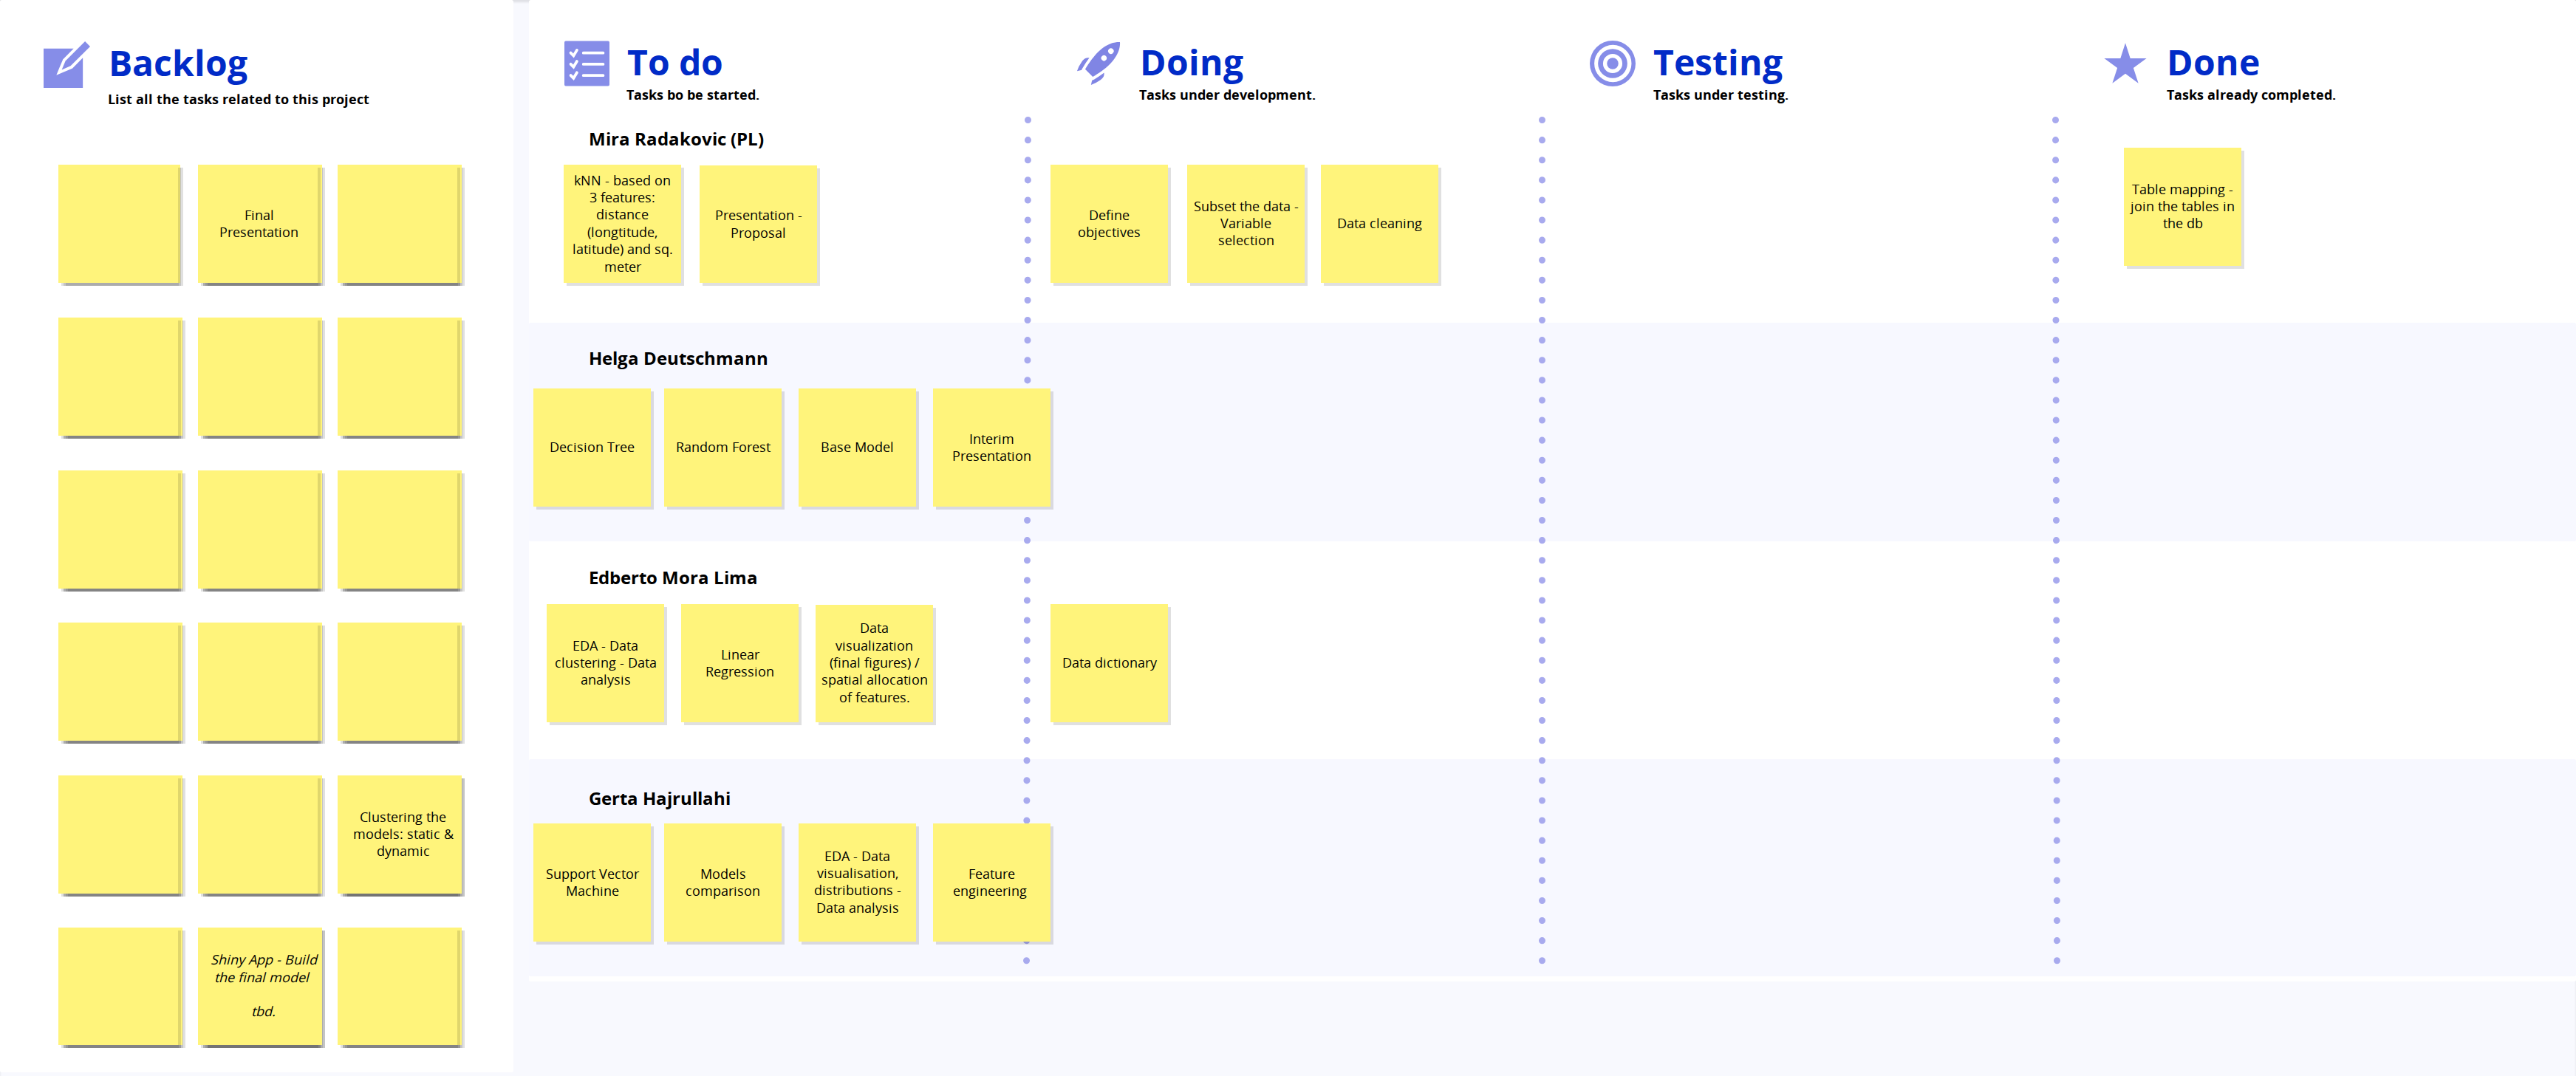
\includegraphics[keepaspectratio]{diagrams/tasks.png}}

}

\caption{\label{fig-kanban-board}Project task tracking board showing
workflow stages from backlog to completion.}

\end{figure}%

\section{Risk Management}\label{risk-management}

\begin{longtable}[]{@{}
  >{\raggedright\arraybackslash}p{(\linewidth - 2\tabcolsep) * \real{0.5000}}
  >{\raggedright\arraybackslash}p{(\linewidth - 2\tabcolsep) * \real{0.5000}}@{}}
\caption{Identified project risks and corresponding mitigation
strategies.}\label{tbl-risks}\tabularnewline
\toprule\noalign{}
\begin{minipage}[b]{\linewidth}\raggedright
Risk
\end{minipage} & \begin{minipage}[b]{\linewidth}\raggedright
Mitigation
\end{minipage} \\
\midrule\noalign{}
\endfirsthead
\toprule\noalign{}
\begin{minipage}[b]{\linewidth}\raggedright
Risk
\end{minipage} & \begin{minipage}[b]{\linewidth}\raggedright
Mitigation
\end{minipage} \\
\midrule\noalign{}
\endhead
\bottomrule\noalign{}
\endlastfoot
Large number of tables / complex joins & Build join pipeline
incrementally; validate row counts at each step \\
Many missing values in building details & Imputation strategies
(median/mode); sensitivity analysis on imputed variables \\
Data covers multiple property types (commercial, mobile homes) & Filter
to Residential Improved sales only at ingestion \\
Temporal drift in prices (market cycles) & Include sale year/month as
features; optionally restrict to recent years \\
Skewed Sale Price distribution & Log-transform target; evaluate models
on both scales \\
Shiny App complexity & Start with minimal viable app; add features
iteratively \\
\end{longtable}

\bookmarksetup{startatroot}

\chapter{Development Plan Overview}\label{development-plan-overview}

The project is splinted into work packages (WP0--WP7) over 6 weeks.

\textbf{Detailed work package specifications} (tasks, deliverables,
quality criteria, and dependencies) are provided in
\href{05-project-schedule-and-workpackages.qmd}{Chapter 5: Project
Schedule \& Work Packages}.

\section{Workflow Diagram}\label{workflow-diagram}

\begin{figure}

\centering{

\pandocbounded{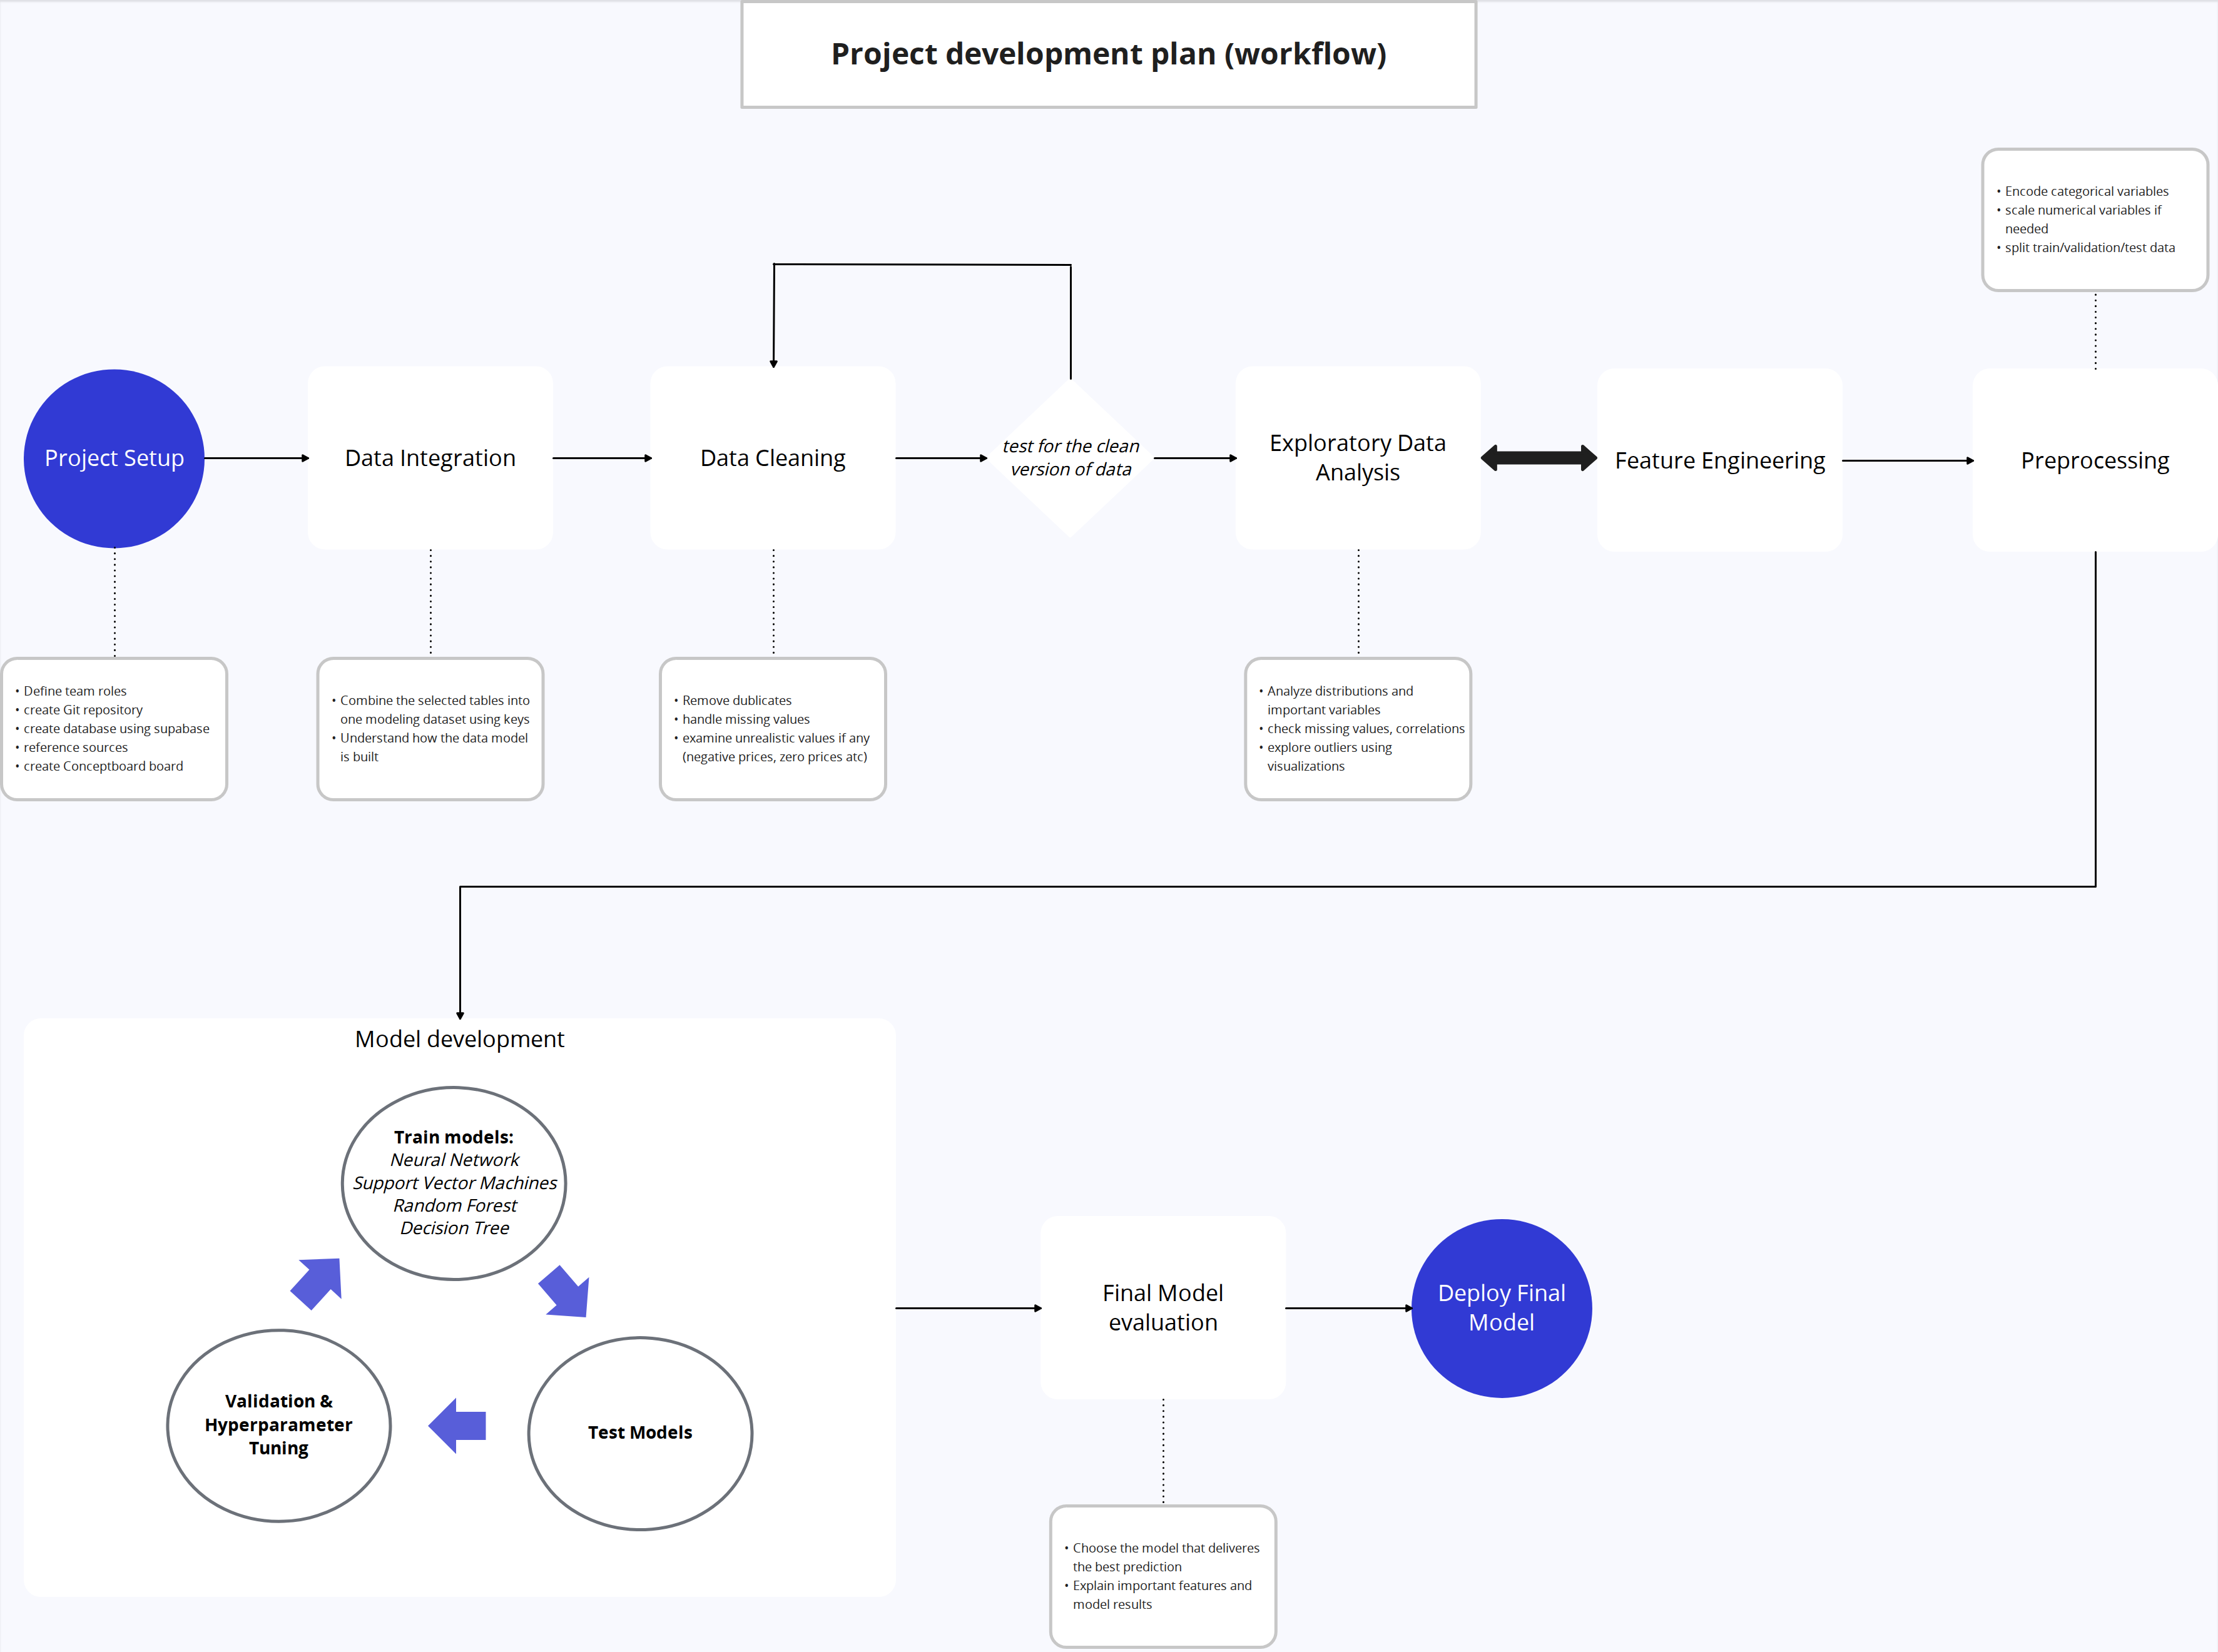
\includegraphics[keepaspectratio]{diagrams/workflow.png}}

}

\caption{\label{fig-workflow}Project Development Workflow}

\end{figure}%

\section{Work Package Summary}\label{work-package-summary}

\begin{longtable}[]{@{}lll@{}}
\caption{High-level work package phases and planned duration in
weeks.}\tabularnewline
\toprule\noalign{}
WP & Phase & Duration \\
\midrule\noalign{}
\endfirsthead
\toprule\noalign{}
WP & Phase & Duration \\
\midrule\noalign{}
\endhead
\bottomrule\noalign{}
\endlastfoot
WP0 & Project Setup & 13--19 May \\
WP1 & Data Integration & 20--26 May \\
WP2 & Data Cleaning & 27 May -- 2 June \\
WP3 & EDA \& Features & 30 May -- 6 June \\
WP4 & Preprocessing & 7--9 June \\
WP5 & Model Development & 9--15 June \\
WP6 & Model Evaluation & 16--20 June \\
WP7 & Deployment & 20--24 June \\
\end{longtable}

\begin{center}\rule{0.5\linewidth}{0.5pt}\end{center}

\section{Communication \& Oversight}\label{communication-oversight}

\textbf{Weekly Sync}:

\begin{itemize}
\item
  Review completed tasks
\item
  Discuss blockers \& dependencies
\item
  Update Kanban board
\item
  Plan next week
\end{itemize}

\textbf{Status Reporting}: Mira provides bi-weekly status to lecturer

\begin{center}\rule{0.5\linewidth}{0.5pt}\end{center}

\bookmarksetup{startatroot}

\chapter{Project Schedule \& Work
Packages}\label{project-schedule-work-packages}

\textbf{Project Duration}: 13 May -- 24 June 2026 (6 weeks)

\begin{center}\rule{0.5\linewidth}{0.5pt}\end{center}

\section{Interactive Gantt Chart}\label{interactive-gantt-chart}

The following chart outlines the project timeline, milestones, and
critical path.

\begin{figure}

\centering{

\pandocbounded{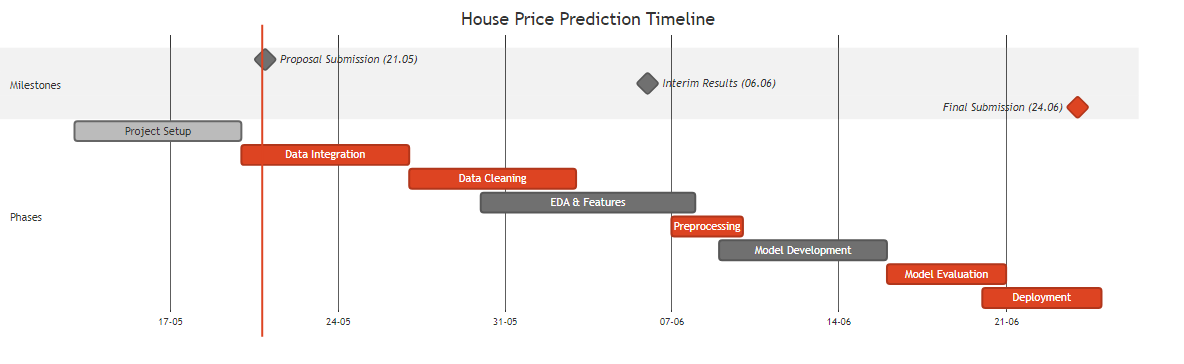
\includegraphics[keepaspectratio]{diagrams/gantt.png}}

}

\caption{\label{fig-gantt-timeline}Project Gantt Chart showing all work
packages and critical path tasks.}

\end{figure}%

\begin{center}\rule{0.5\linewidth}{0.5pt}\end{center}

\section{Detailed Work Package
Definitions}\label{detailed-work-package-definitions}

\subsection{WP0: Project Setup}\label{wp0-project-setup}

\textbf{Duration}: 13--19 May \textbar{} \textbf{Status}: Done

\subsubsection{Tasks}\label{tasks}

\begin{enumerate}
\def\labelenumi{\arabic{enumi}.}
\tightlist
\item
  Define team roles and responsibilities
\item
  Create Git repository (private, shared with lecturer)
\item
  Set up Supabase database connection
\item
  Initialize Kanban board (Backlog/To Do/Doing/Testing/Done)
\item
  Configure R development environment
\end{enumerate}

\subsubsection{Deliverables}\label{deliverables}

\begin{itemize}
\tightlist
\item
  GitHub repository
\item
  Supabase connection
\item
  Kanban board
\item
  Team charter document
\end{itemize}

\begin{center}\rule{0.5\linewidth}{0.5pt}\end{center}

\subsection{WP1: Data Integration}\label{wp1-data-integration}

\textbf{Duration}: 20--26 May \textbar{} \textbf{Status}: Partially
complete

\subsubsection{Tasks}\label{tasks-1}

\begin{enumerate}
\def\labelenumi{\arabic{enumi}.}
\tightlist
\item
  Download Pierce County data files
\item
  Map table relationships and join keys
\item
  Perform sequential table joins (validate at each step)
\item
  Validate referential integrity and row counts
\item
  Create data integration report
\end{enumerate}

\subsubsection{Deliverables}\label{deliverables-1}

\begin{itemize}
\tightlist
\item
  Integrated dataset (.RData)
\item
  Table mapping diagram
\item
  Data dictionary
\item
  Validation report with row counts
\end{itemize}

\subsubsection{Quality Criteria}\label{quality-criteria}

\begin{itemize}
\tightlist
\item[$\square$]
  All tables joined successfully
\item[$\square$]
  Row counts documented at each step
\item[$\square$]
  No unexpected NULL values
\item[$\square$]
  Referential integrity verified
\end{itemize}

\begin{center}\rule{0.5\linewidth}{0.5pt}\end{center}

\subsection{WP2: Data Cleaning \&
Preparation}\label{wp2-data-cleaning-preparation}

\textbf{Duration}: 27 May -- 2 June \textbar{} \textbf{Status}: To Do

\subsubsection{Tasks}\label{tasks-2}

\begin{enumerate}
\def\labelenumi{\arabic{enumi}.}
\tightlist
\item
  Filter to Residential Improved properties only
\item
  Remove duplicate records
\item
  Handle missing values (document strategy)
\item
  Examine and document outliers
\item
  Variable selection --- keep only analysis-ready columns
\item
  Run validation test suite
\end{enumerate}

\subsubsection{Deliverables}\label{deliverables-2}

\begin{itemize}
\tightlist
\item
  Cleaned dataset (.RData)
\item
  Data cleaning log
\item
  Missing value analysis
\item
  Quality assurance report
\end{itemize}

\subsubsection{Quality Criteria}\label{quality-criteria-1}

\begin{itemize}
\tightlist
\item[$\square$]
  No critical missing values
\item[$\square$]
  Data types verified
\item[$\square$]
  Outliers documented
\item[$\square$]
  Test suite passes
\end{itemize}

\begin{center}\rule{0.5\linewidth}{0.5pt}\end{center}

\subsection{WP3: Exploratory Data Analysis \& Feature
Engineering}\label{wp3-exploratory-data-analysis-feature-engineering}

\textbf{Duration}: 30 May -- 9 June \textbar{} \textbf{Status}: To Do

\subsubsection{WP3a: EDA Tasks}\label{wp3a-eda-tasks}

\begin{itemize}
\tightlist
\item
  Univariate analysis (distributions, summaries)
\item
  Bivariate analysis (price vs.~key variables)
\item
  Spatial analysis with leaflet maps
\item
  Correlation matrix and hypothesis testing
\end{itemize}

\subsubsection{WP3b: Feature Engineering
Tasks}\label{wp3b-feature-engineering-tasks}

\begin{itemize}
\tightlist
\item
  Create derived features (age, price/sqft, neighborhood effects, etc.)
\item
  Encode categorical variables
\item
  Feature selection --- target ≥15 final features
\item
  Document feature importance baseline
\end{itemize}

\subsubsection{Deliverables}\label{deliverables-3}

\begin{itemize}
\tightlist
\item
  EDA report with visualizations
\item
  Correlation heatmap
\item
  Feature engineering log
\item
  Final feature set documentation (≥15 features)
\end{itemize}

\subsubsection{Quality Criteria}\label{quality-criteria-2}

\begin{itemize}
\tightlist
\item[$\square$]
  All visualizations publication-ready
\item[$\square$]
  ≥15 features engineered and named
\item[$\square$]
  No data leakage from target variable
\item[$\square$]
  Feature-target correlations documented
\end{itemize}

\begin{center}\rule{0.5\linewidth}{0.5pt}\end{center}

\subsection{WP4: Preprocessing}\label{wp4-preprocessing}

\textbf{Duration}: 7--9 June \textbar{} \textbf{Status}: To Do

\subsubsection{Tasks}\label{tasks-3}

\begin{enumerate}
\def\labelenumi{\arabic{enumi}.}
\tightlist
\item
  Encode categorical variables (finalize encoding scheme)
\item
  Scale numerical variables (standardize or normalize)
\item
  Train/validation/test split (70/15/15\% stratified)
\item
  Document random seed for reproducibility
\end{enumerate}

\subsubsection{Deliverables}\label{deliverables-4}

\begin{itemize}
\tightlist
\item
  3 split datasets (train, validation, test)
\item
  Encoding mapping tables
\item
  Scaling parameters (saved as R object)
\item
  Data split documentation
\end{itemize}

\subsubsection{Quality Criteria}\label{quality-criteria-3}

\begin{itemize}
\tightlist
\item[$\square$]
  No data leakage (scaling only from training set)
\item[$\square$]
  Balanced distribution across splits
\item[$\square$]
  Random seed documented
\item[$\square$]
  All features properly encoded/scaled
\end{itemize}

\begin{center}\rule{0.5\linewidth}{0.5pt}\end{center}

\subsection{WP5: Model Development (Parallel
Tracks)}\label{wp5-model-development-parallel-tracks}

\textbf{Duration}: 9--15 June \textbar{} \textbf{Status}: To Do

\subsubsection{WP5a: Baseline \& Tree
Models}\label{wp5a-baseline-tree-models}

\begin{itemize}
\tightlist
\item
  Baseline Linear Regression
\item
  Decision Tree (hyperparameter tuning)
\item
  Random Forest (grid search over parameters)
\end{itemize}

\subsubsection{WP5b: Support Vector
Machine}\label{wp5b-support-vector-machine}

\begin{itemize}
\tightlist
\item
  SVM setup (kernel selection)
\item
  Hyperparameter tuning (C, epsilon)
\item
  Cross-validation
\end{itemize}

\subsubsection{WP5c: k-Nearest
Neighbours}\label{wp5c-k-nearest-neighbours}

\begin{itemize}
\tightlist
\item
  Setup (distance metric, k selection)
\item
  kNN based on: distance (lon, lat) + square metre
\item
  Hyperparameter optimization
\end{itemize}

\subsubsection{WP5d: Linear Regression}\label{wp5d-linear-regression}

\begin{itemize}
\tightlist
\item
  Full feature set training
\item
  Feature importance extraction
\item
  Residual diagnostics
\end{itemize}

\subsubsection{Deliverables}\label{deliverables-5}

\begin{itemize}
\tightlist
\item
  Trained model objects (.RDS)
\item
  Cross-validation results
\item
  Validation \& test metrics
\item
  Model configuration documentation
\end{itemize}

\subsubsection{Quality Criteria}\label{quality-criteria-4}

\begin{itemize}
\tightlist
\item[$\square$]
  All 5 models trained and saved
\item[$\square$]
  Cross-validation RMSE \textless{} 100k (preliminary)
\item[$\square$]
  No data leakage to validation/test
\item[$\square$]
  Test predictions generated for all samples
\end{itemize}

\begin{center}\rule{0.5\linewidth}{0.5pt}\end{center}

\subsection{WP6: Model Evaluation \&
Selection}\label{wp6-model-evaluation-selection}

\textbf{Duration}: 16--20 June \textbar{} \textbf{Status}: To Do

\subsubsection{Tasks}\label{tasks-4}

\begin{enumerate}
\def\labelenumi{\arabic{enumi}.}
\tightlist
\item
  Cross-validation for all 5 models (k=5 fold)
\item
  Performance benchmarking (RMSE, MAE, R²)
\item
  Create model comparison table and visualizations
\item
  Select best model based on criteria:

  \begin{itemize}
  \tightlist
  \item
    RMSE \textless{} USD 80,000
  \item
    R² \textgreater{} 0.80
  \end{itemize}
\item
  Extract and visualize feature importance
\end{enumerate}

\subsubsection{Deliverables}\label{deliverables-6}

\begin{itemize}
\tightlist
\item
  Model comparison table (CSV)
\item
  Benchmarking plots (PNG/PDF)
\item
  Best model selection report
\item
  Feature importance ranking
\item
  Final model object saved
\end{itemize}

\subsubsection{Quality Criteria}\label{quality-criteria-5}

\begin{itemize}
\tightlist
\item[$\square$]
  All models evaluated on same test set
\item[$\square$]
  Best model meets RMSE \textless{} 80k \& R² \textgreater{} 0.80
  targets
\item[$\square$]
  Feature importance interpreted
\item[$\square$]
  Selection criteria documented
\end{itemize}

\begin{center}\rule{0.5\linewidth}{0.5pt}\end{center}

\subsection{WP7: Deployment \&
Documentation}\label{wp7-deployment-documentation}

\textbf{Duration}: 20--24 June \textbar{} \textbf{Status}: To Do

\subsubsection{Tasks}\label{tasks-5}

\begin{enumerate}
\def\labelenumi{\arabic{enumi}.}
\tightlist
\item
  Build Shiny App (UI + server logic)
\item
  Create prediction endpoint (returns estimate + confidence interval)
\item
  Add feature importance visualization
\item
  Final validation testing
\item
  Prepare presentation slides
\item
  Assemble final report
\item
  Deploy to shinyapps.io or local server
\end{enumerate}

\subsubsection{Deliverables}\label{deliverables-7}

\begin{itemize}
\tightlist
\item
  Deployed Shiny App
\item
  App source code (app.R)
\item
  Presentation slides (PDF)
\item
  Final report (PDF)
\item
  User guide \& model documentation
\item
  All code on GitHub
\end{itemize}

\subsubsection{Quality Criteria}\label{quality-criteria-6}

\begin{itemize}
\tightlist
\item[$\square$]
  Shiny App loads without errors
\item[$\square$]
  Predictions return in \textless5 seconds
\item[$\square$]
  Confidence intervals displayed
\item[$\square$]
  Presentation covers all key findings
\item[$\square$]
  Report submitted via Moodle by deadline
\end{itemize}

\begin{center}\rule{0.5\linewidth}{0.5pt}\end{center}

\section{Dependencies \& Critical
Path}\label{dependencies-critical-path}

\begin{longtable}[]{@{}lll@{}}
\caption{Work package interdependencies and blocking relationships
defining the critical path.}\label{tbl-dependencies}\tabularnewline
\toprule\noalign{}
WP & Depends On & Notes \\
\midrule\noalign{}
\endfirsthead
\toprule\noalign{}
WP & Depends On & Notes \\
\midrule\noalign{}
\endhead
\bottomrule\noalign{}
\endlastfoot
WP1 & WP0 & Requires Git repo \& Supabase setup \\
WP2 & WP1 & Requires integrated dataset \\
WP3 & WP2 & Requires clean dataset \\
WP4 & WP3 & Requires feature set \\
WP5 & WP4 & Requires preprocessed data \\
WP6 & WP5 & Requires all trained models \\
WP7 & WP6 & Requires selected best model \\
\end{longtable}

\textbf{Critical Path Tasks}: 1. WP1: Data integration (26.05) 2. WP2:
Data cleaning (02.06) 3. WP3: Feature engineering (09.06) 4. WP4:
Train/test split (09.06) 5. WP5: Model training (15.06) 6. WP6: Model
selection (20.06) 7. WP7: Shiny App deployment (23.06)

\begin{center}\rule{0.5\linewidth}{0.5pt}\end{center}

\section{Key Milestones}\label{key-milestones}

\begin{longtable}[]{@{}
  >{\raggedright\arraybackslash}p{(\linewidth - 4\tabcolsep) * \real{0.3333}}
  >{\raggedright\arraybackslash}p{(\linewidth - 4\tabcolsep) * \real{0.3333}}
  >{\raggedright\arraybackslash}p{(\linewidth - 4\tabcolsep) * \real{0.3333}}@{}}
\caption{Project milestones, scheduled events, and corresponding
deliverables.}\label{tbl-milestones}\tabularnewline
\toprule\noalign{}
\begin{minipage}[b]{\linewidth}\raggedright
Date
\end{minipage} & \begin{minipage}[b]{\linewidth}\raggedright
Event
\end{minipage} & \begin{minipage}[b]{\linewidth}\raggedright
Deliverables
\end{minipage} \\
\midrule\noalign{}
\endfirsthead
\toprule\noalign{}
\begin{minipage}[b]{\linewidth}\raggedright
Date
\end{minipage} & \begin{minipage}[b]{\linewidth}\raggedright
Event
\end{minipage} & \begin{minipage}[b]{\linewidth}\raggedright
Deliverables
\end{minipage} \\
\midrule\noalign{}
\endhead
\bottomrule\noalign{}
\endlastfoot
\textbf{21.05.2026} & Proposal Presentation & Objectives, data
dictionary, organization, development plan \\
\textbf{06.06.2026} & Interim Results & Data status, EDA findings,
initial model results \\
\textbf{18.06.2026} & Feedback Round & Review feedback, adjust if
needed \\
\textbf{24.06.2026} & Final Presentation & Live demo + report submission
via Moodle \\
\end{longtable}

\begin{center}\rule{0.5\linewidth}{0.5pt}\end{center}

\section{Weekly Status Checklist}\label{weekly-status-checklist}

\begin{itemize}
\tightlist
\item[$\boxtimes$]
  \textbf{Week 1 (13--19.05)}: WP0 setup complete
\item[$\boxtimes$]
  \textbf{Week 2 (20--26.05)}: WP1 data integration done, Proposal
  prepared
\item[$\boxtimes$]
  \textbf{Week 3 (27.05--02.06)}: WP2 data cleaning complete, WP3
  started
\item[$\boxtimes$]
  \textbf{Week 4 (03--09.06)}: WP3 features complete, WP4 preprocessing
  ready
\item[$\boxtimes$]
  \textbf{Week 5 (10--16.06)}: WP5 all 5 models trained and validated
\item[$\boxtimes$]
  \textbf{Week 6 (17--23.06)}: WP6 best model selected, WP7 Shiny App
  deployed
\item[$\boxtimes$]
  \textbf{Week 7 (24.06)}: Final presentation \& report submitted
\end{itemize}

\bookmarksetup{startatroot}

\chapter{EDA Summary}\label{eda-summary}

\section{EDA Summary}\label{eda-summary-1}

File saved under:
/workspaces/SOE-R-House-Price-Prediction/analysis/00-eda-analysis/eda.qmd

Before performing the final exploratory analysis, several data
preparation and cleaning steps were completed. The goal was to create a
clean, meaningful, and residential-focused dataset that can later be
used for house price prediction.

\subsection{Step 1: Loaded and described the raw data
sources}\label{step-1-loaded-and-described-the-raw-data-sources}

The project started by loading several property-related text files. Each
file represented a different part of the property data:

\begin{itemize}
\item
  sales transactions
\item
  appraisal account information
\item
  improvement/building information
\item
  improvement built-as information
\item
  improvement detail information
\item
  land attributes
\item
  parcel segregation and merge history
\item
  tax account information
\end{itemize}

Because the raw text files did not contain column headers, meaningful
column names were manually assigned based on the official data
documentation.

\subsection{Step 2: Checked basic data
quality}\label{step-2-checked-basic-data-quality}

A data quality check was performed for each table. This included
checking:

\begin{itemize}
\item
  number of rows
\item
  number of columns
\item
  duplicate rows
\item
  total missing values
\item
  number of columns with missing values
\end{itemize}

The data quality check showed that there were no full duplicate rows in
the original tables. However, several columns contained missing values
and needed further inspection.

\subsection{Step 3: Checked repeated parcel
numbers}\label{step-3-checked-repeated-parcel-numbers}

The \texttt{parcel\_number} variable was checked because it is the main
key used to connect the data sources.

This step showed that some tables contain repeated parcel numbers, while
others contain only one row per parcel. This was important because
repeated parcel numbers can create one-to-many relationships during
joins.

\subsection{Step 4: Analyzed missing values by
column}\label{step-4-analyzed-missing-values-by-column}

Missing values were inspected at the column level. Columns with very
high missingness were identified and reviewed.

Several variables with more than 80\% missing values were removed
because they were unlikely to provide reliable information for analysis
or modeling.

Examples include:

\begin{itemize}
\item
  \texttt{waterfront\_type}
\item
  \texttt{view\_quality}
\item
  \texttt{group\_account\_number}
\item
  \texttt{business\_name}
\item
  \texttt{submerged\_area\_square\_feet}
\item
  mobile-home-specific variables
\item
  basement and garage-related variables with very high missingness
\item
  exemption and current-use-code variables in the tax table
\end{itemize}

\subsection{Step 5: Removed high-missing
columns}\label{step-5-removed-high-missing-columns}

After reviewing missingness, selected columns were removed from the
appraisal account, improvement, improvement built-as, and tax account
tables.

This reduced noise and made the dataset more suitable for analysis.

\subsection{Step 6: Filtered valid and confirmed
sales}\label{step-6-filtered-valid-and-confirmed-sales}

The sales table was filtered to keep only transactions that were:

\begin{itemize}
\item
  valid
\item
  confirmed
\item
  not excluded
\item
  not missing sale price
\item
  greater than zero
\end{itemize}

This step was important because the target variable,
\texttt{sale\_price}, should represent normal market transactions as
much as possible.

\subsection{Step 7: Joined the data
sources}\label{step-7-joined-the-data-sources}

The cleaned tables were joined into one analysis dataset.

The sales table was used as the base table because it contains the
target variable, \texttt{sale\_price}. Other tables were joined using
\texttt{parcel\_number} and, where necessary, \texttt{building\_id}.

Some row duplication after joining was expected because several tables
contain multiple records per parcel or building.

\subsection{Step 8: Removed columns with no useful
variation}\label{step-8-removed-columns-with-no-useful-variation}

After joining the data, the number of unique values was checked for each
column.

Columns with only one unique value were removed because they do not
provide useful information for analysis or modeling.

\subsection{Step 9: Removed identifier and irrelevant
columns}\label{step-9-removed-identifier-and-irrelevant-columns}

Several columns were removed because they were identifiers,
administrative fields, detailed text labels, or variables not useful for
prediction.

Examples include:

\begin{itemize}
\item
  transaction IDs
\item
  parcel IDs
\item
  building IDs
\item
  grantor and grantee names
\item
  site address
\item
  tax area codes
\item
  subdivision name
\item
  raw descriptive text fields that were replaced by grouped variables
\end{itemize}

\subsection{Step 10: Engineered grouped categorical
features}\label{step-10-engineered-grouped-categorical-features}

Several detailed categorical variables were simplified into broader
groups.

This made the dataset easier to interpret and reduced the number of
categories.

The main grouped features were:

\begin{itemize}
\item
  \texttt{utility\_electric}
\item
  \texttt{utility\_sewer}
\item
  \texttt{utility\_water}
\item
  \texttt{street\_type}
\item
  \texttt{primary\_occupancy\_group}
\item
  \texttt{hvac\_group}
\item
  \texttt{detail\_group}
\item
  \texttt{use\_group}
\end{itemize}

\subsection{Step 11: Created boolean amenity
features}\label{step-11-created-boolean-amenity-features}

The detailed improvement descriptions were used to create boolean
features that indicate whether certain property features are present.

The created amenity indicators include:

\begin{itemize}
\item
  \texttt{has\_bath\_detail}
\item
  \texttt{has\_garage\_or\_carport\_detail}
\item
  \texttt{has\_deck\_or\_porch\_detail}
\item
  \texttt{has\_pool\_or\_spa\_detail}
\item
  \texttt{has\_fireplace\_detail}
\item
  \texttt{has\_storage\_detail}
\item
  \texttt{has\_waterfront\_detail}
\item
  \texttt{has\_parking\_detail}
\item
  \texttt{has\_finished\_space\_detail}
\end{itemize}

These features helped turn complex text descriptions into simpler
variables that can be used in analysis and modeling.

\subsection{Step 12: Converted date
variables}\label{step-12-converted-date-variables}

The date columns were converted into proper date format.

The most important date variable was \texttt{sale\_date}, which was
later used to create \texttt{sale\_year}.

This allowed the analysis of sale price trends over time.

\subsection{Step 13: Checked categorical redundancy with Cramér's
V}\label{step-13-checked-categorical-redundancy-with-cramuxe9rs-v}

Cramér's V was used to examine associations between categorical
variables.

This helped identify categorical variables that contained overlapping or
redundant information.

Based on this analysis, several categorical variables were removed,
especially those that were administrative, duplicated information, or
replaced by grouped versions.

\subsection{Step 14: Checked numeric redundancy with
correlations}\label{step-14-checked-numeric-redundancy-with-correlations}

A numeric correlation matrix was used to check relationships between
numeric variables.

This helped identify highly correlated variables and variables that
could create multicollinearity.

Assessor-value variables were also removed because they may leak
information about the target variable \texttt{sale\_price}.

Examples of removed numeric variables include:

\begin{itemize}
\item
  prior and current assessed land values
\item
  prior and current improvement values
\item
  total market values
\item
  taxable values
\item
  redundant land-size variables
\item
  redundant building-age variables
\end{itemize}

\subsection{Step 15: Checked variance and numeric
summaries}\label{step-15-checked-variance-and-numeric-summaries}

The remaining numeric variables were summarized using:

\begin{itemize}
\item
  missing values
\item
  number of unique values
\item
  minimum
\item
  maximum
\item
  mean
\item
  median
\item
  standard deviation
\item
  variance
\end{itemize}

This helped identify unusual distributions, low-variation variables, and
potential issues before the final EDA.

\subsection{Step 16: Consolidated overlapping
features}\label{step-16-consolidated-overlapping-features}

Some related features were combined to reduce redundancy.

For example:

\begin{itemize}
\item
  fireplace count was combined with fireplace detail information
\item
  bathroom detail was compared with numeric bathroom count
\item
  porch detail was compared with porch square footage
\item
  garage detail was compared with attached garage square footage
\end{itemize}

This ensured that useful information was kept while redundant variables
were removed.

\subsection{Step 17: Focused the analysis on residential
properties}\label{step-17-focused-the-analysis-on-residential-properties}

The sale price analysis showed that very high sale prices were often
linked to commercial, industrial, or multi-unit properties.

Since the project focuses on house price prediction, the dataset was
filtered to include only residential properties.

The final residential dataset kept records where:

\begin{itemize}
\item
  \texttt{property\_type\ ==\ "Residential"}
\item
  \texttt{use\_group\ ==\ "Residential"}
\item
  \texttt{sale\_price\ \textgreater{}=\ 10000}
\end{itemize}

This made the dataset more relevant for predicting residential house
prices.

\subsection{Step 18: Removed low-variation variables after residential
filtering}\label{step-18-removed-low-variation-variables-after-residential-filtering}

After filtering to residential properties, some variables became highly
imbalanced and were removed.

These included utility and access variables, because almost all
residential properties had electric, water, sewer/septic, and road
access.

Other less useful or redundant variables were also removed at this
stage.

\subsection{Step 19: Created the final feature
set}\label{step-19-created-the-final-feature-set}

After all cleaning, grouping, filtering, and redundancy checks, a final
dataset was created for EDA and later modeling.

The final dataset includes variables related to:

\begin{itemize}
\item
  sale date and sale year
\item
  sale price
\item
  location
\item
  neighborhood
\item
  land size
\item
  building size
\item
  quality
\item
  exterior
\item
  stories
\item
  bedrooms
\item
  bathrooms
\item
  units
\item
  year built
\item
  HVAC group
\item
  primary occupancy group
\item
  garage, porch, pool, storage, waterfront, and finished-space
  indicators
\end{itemize}

\subsection{Step 20: Performed final exploratory data
analysis}\label{step-20-performed-final-exploratory-data-analysis}

The final EDA focused on understanding the residential dataset.

The main analyses included:

\begin{itemize}
\item
  sale price distribution
\item
  sale price outliers
\item
  sale price trends over time
\item
  numeric feature correlations with sale price
\item
  numeric feature visualizations
\item
  categorical feature comparisons
\item
  boolean amenity feature comparisons
\item
  location-based price patterns
\item
  missing values in the final dataset
\item
  interactions between important variables
\end{itemize}

These steps helped identify the most relevant variables for later
modeling and showed that sale price is influenced by time, location,
building size, quality, room count, land size, and selected amenities.

\section{Most Important EDA Findings}\label{most-important-eda-findings}

\subsection{Finding 1: Sale prices are strongly
right-skewed}\label{finding-1-sale-prices-are-strongly-right-skewed}

The sale price distribution shows a strong right skew. Most residential
properties are concentrated in the lower and middle price ranges, while
a smaller number of expensive properties create a long right tail.

\begin{figure}[H]

{\centering \pandocbounded{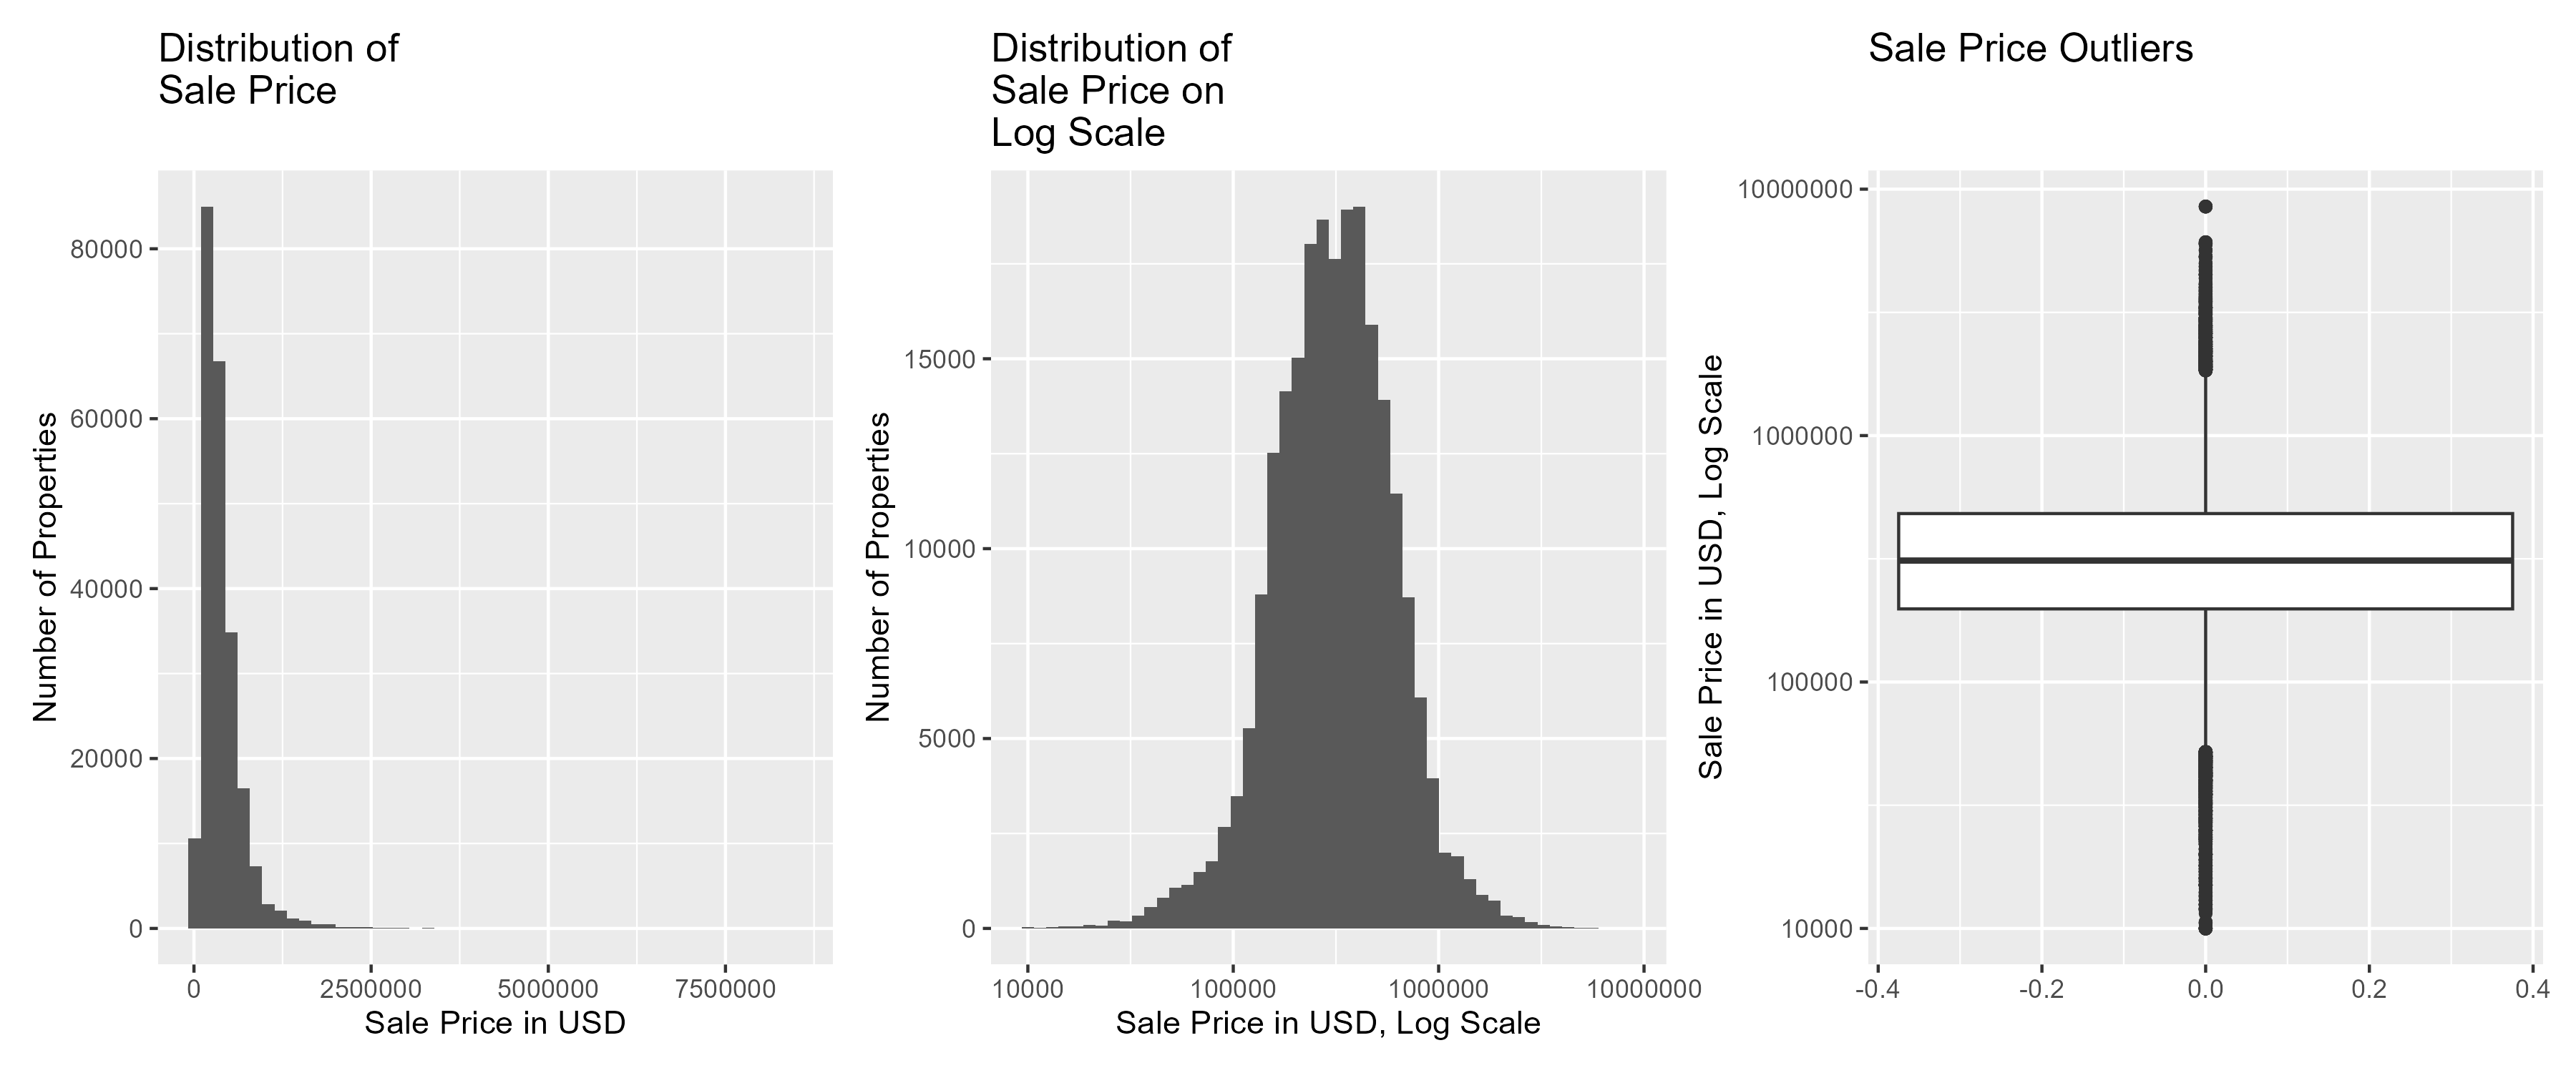
\includegraphics[keepaspectratio]{diagrams/eda/01_sale_price_distribution_outliers.png}}

}

\caption{Sales price distribution}

\end{figure}%

The log-scale histogram makes the distribution easier to interpret
because it reduces the visual impact of extreme high values. The boxplot
confirms that high-value outliers are still present. This suggests that
a log transformation of \texttt{sale\_price} should be considered during
modeling.

\subsection{Finding 2: Median sale prices increased strongly over
time}\label{finding-2-median-sale-prices-increased-strongly-over-time}

The median sale price shows a clear upward trend over time. Prices
increased gradually from the late 1990s to the mid-2000s, declined
around the 2008--2010 period, and then increased again.

\begin{figure}[H]

{\centering \pandocbounded{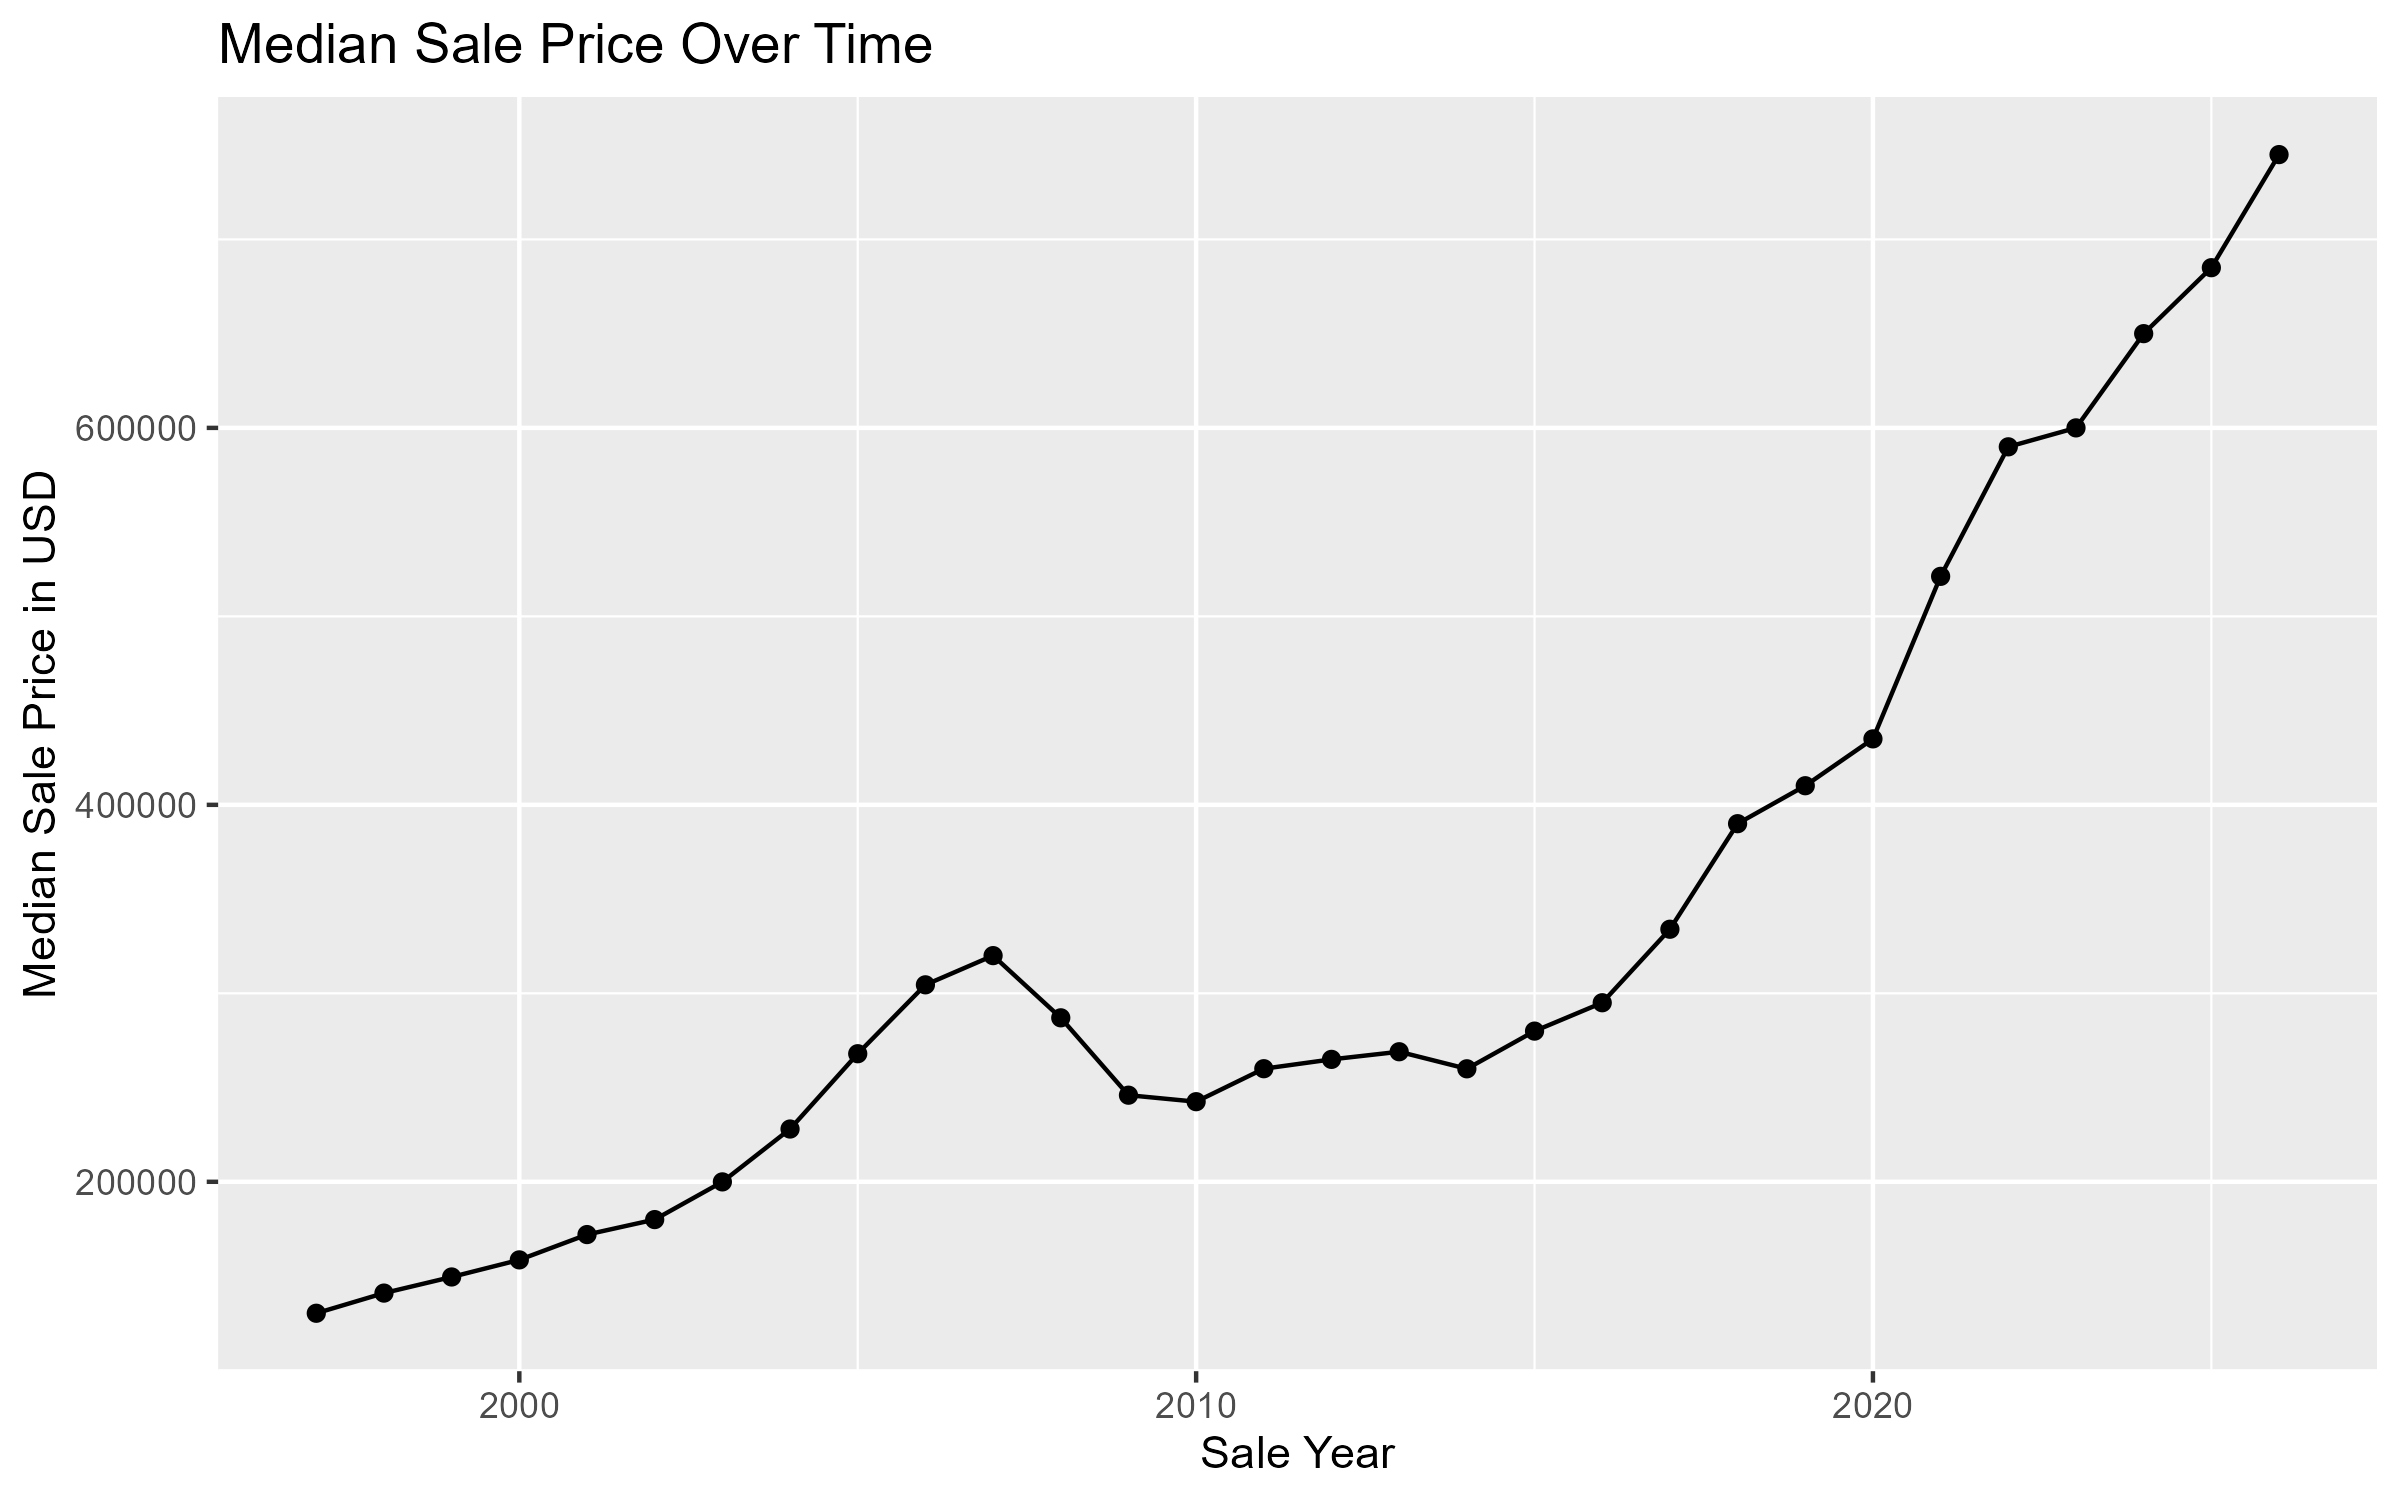
\includegraphics[keepaspectratio]{diagrams/eda/02_median_sale_price_over_time.png}}

}

\caption{Sale Price over Time}

\end{figure}%

The strongest increase appears after approximately 2015, with median
prices reaching their highest levels in the most recent years. This
shows that \texttt{sale\_year} is an important predictor because it
captures market changes over time.

\subsection{Finding 3: Sale year, building size, bathrooms, and porch
size have the strongest numeric relationships with sale
price}\label{finding-3-sale-year-building-size-bathrooms-and-porch-size-have-the-strongest-numeric-relationships-with-sale-price}

The correlation analysis shows that \texttt{sale\_year} has the
strongest positive correlation with \texttt{sale\_price}. This confirms
that time is one of the most important numeric predictors.

\begin{figure}[H]

{\centering \pandocbounded{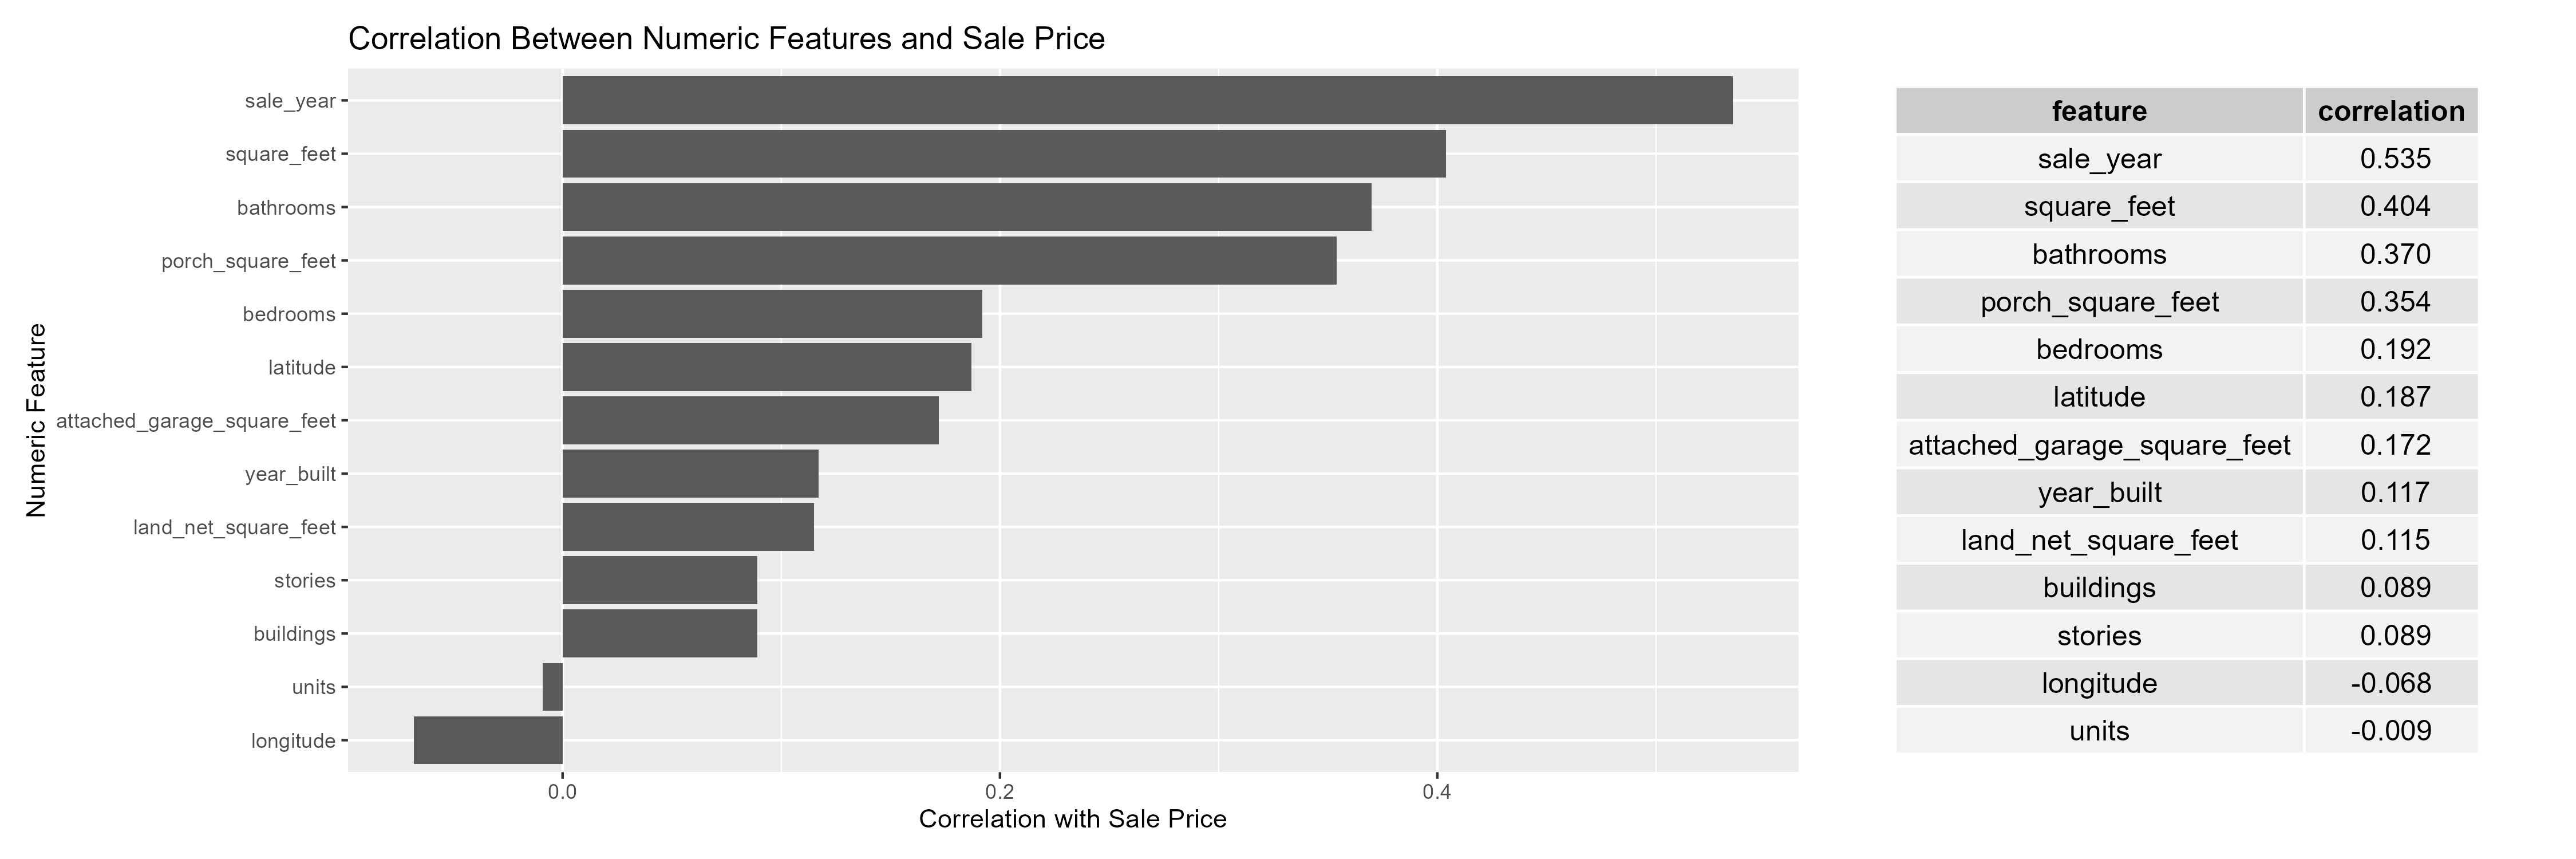
\includegraphics[keepaspectratio]{diagrams/eda/03_numeric_feature_correlations.png}}

}

\caption{Numeric Feature Correlation}

\end{figure}%

Building size, represented by \texttt{square\_feet}, also has a clear
positive relationship with sale price. Other important numeric variables
include \texttt{bathrooms}, \texttt{porch\_square\_feet},
\texttt{bedrooms}, \texttt{latitude},
\texttt{attached\_garage\_square\_feet}, \texttt{year\_built}, and
\texttt{land\_net\_square\_feet}.

The correlations are moderate rather than extremely high. This means
that sale price is not explained by one variable alone, but by a
combination of time, size, location, room count, land size, and property
characteristics.

\subsection{Finding 4: Larger and better-equipped homes generally have
higher sale
prices}\label{finding-4-larger-and-better-equipped-homes-generally-have-higher-sale-prices}

The numeric feature visualizations show several important relationships.
Larger homes generally have higher sale prices, although there is still
a wide spread in prices for similar building sizes.

\begin{figure}[H]

{\centering \pandocbounded{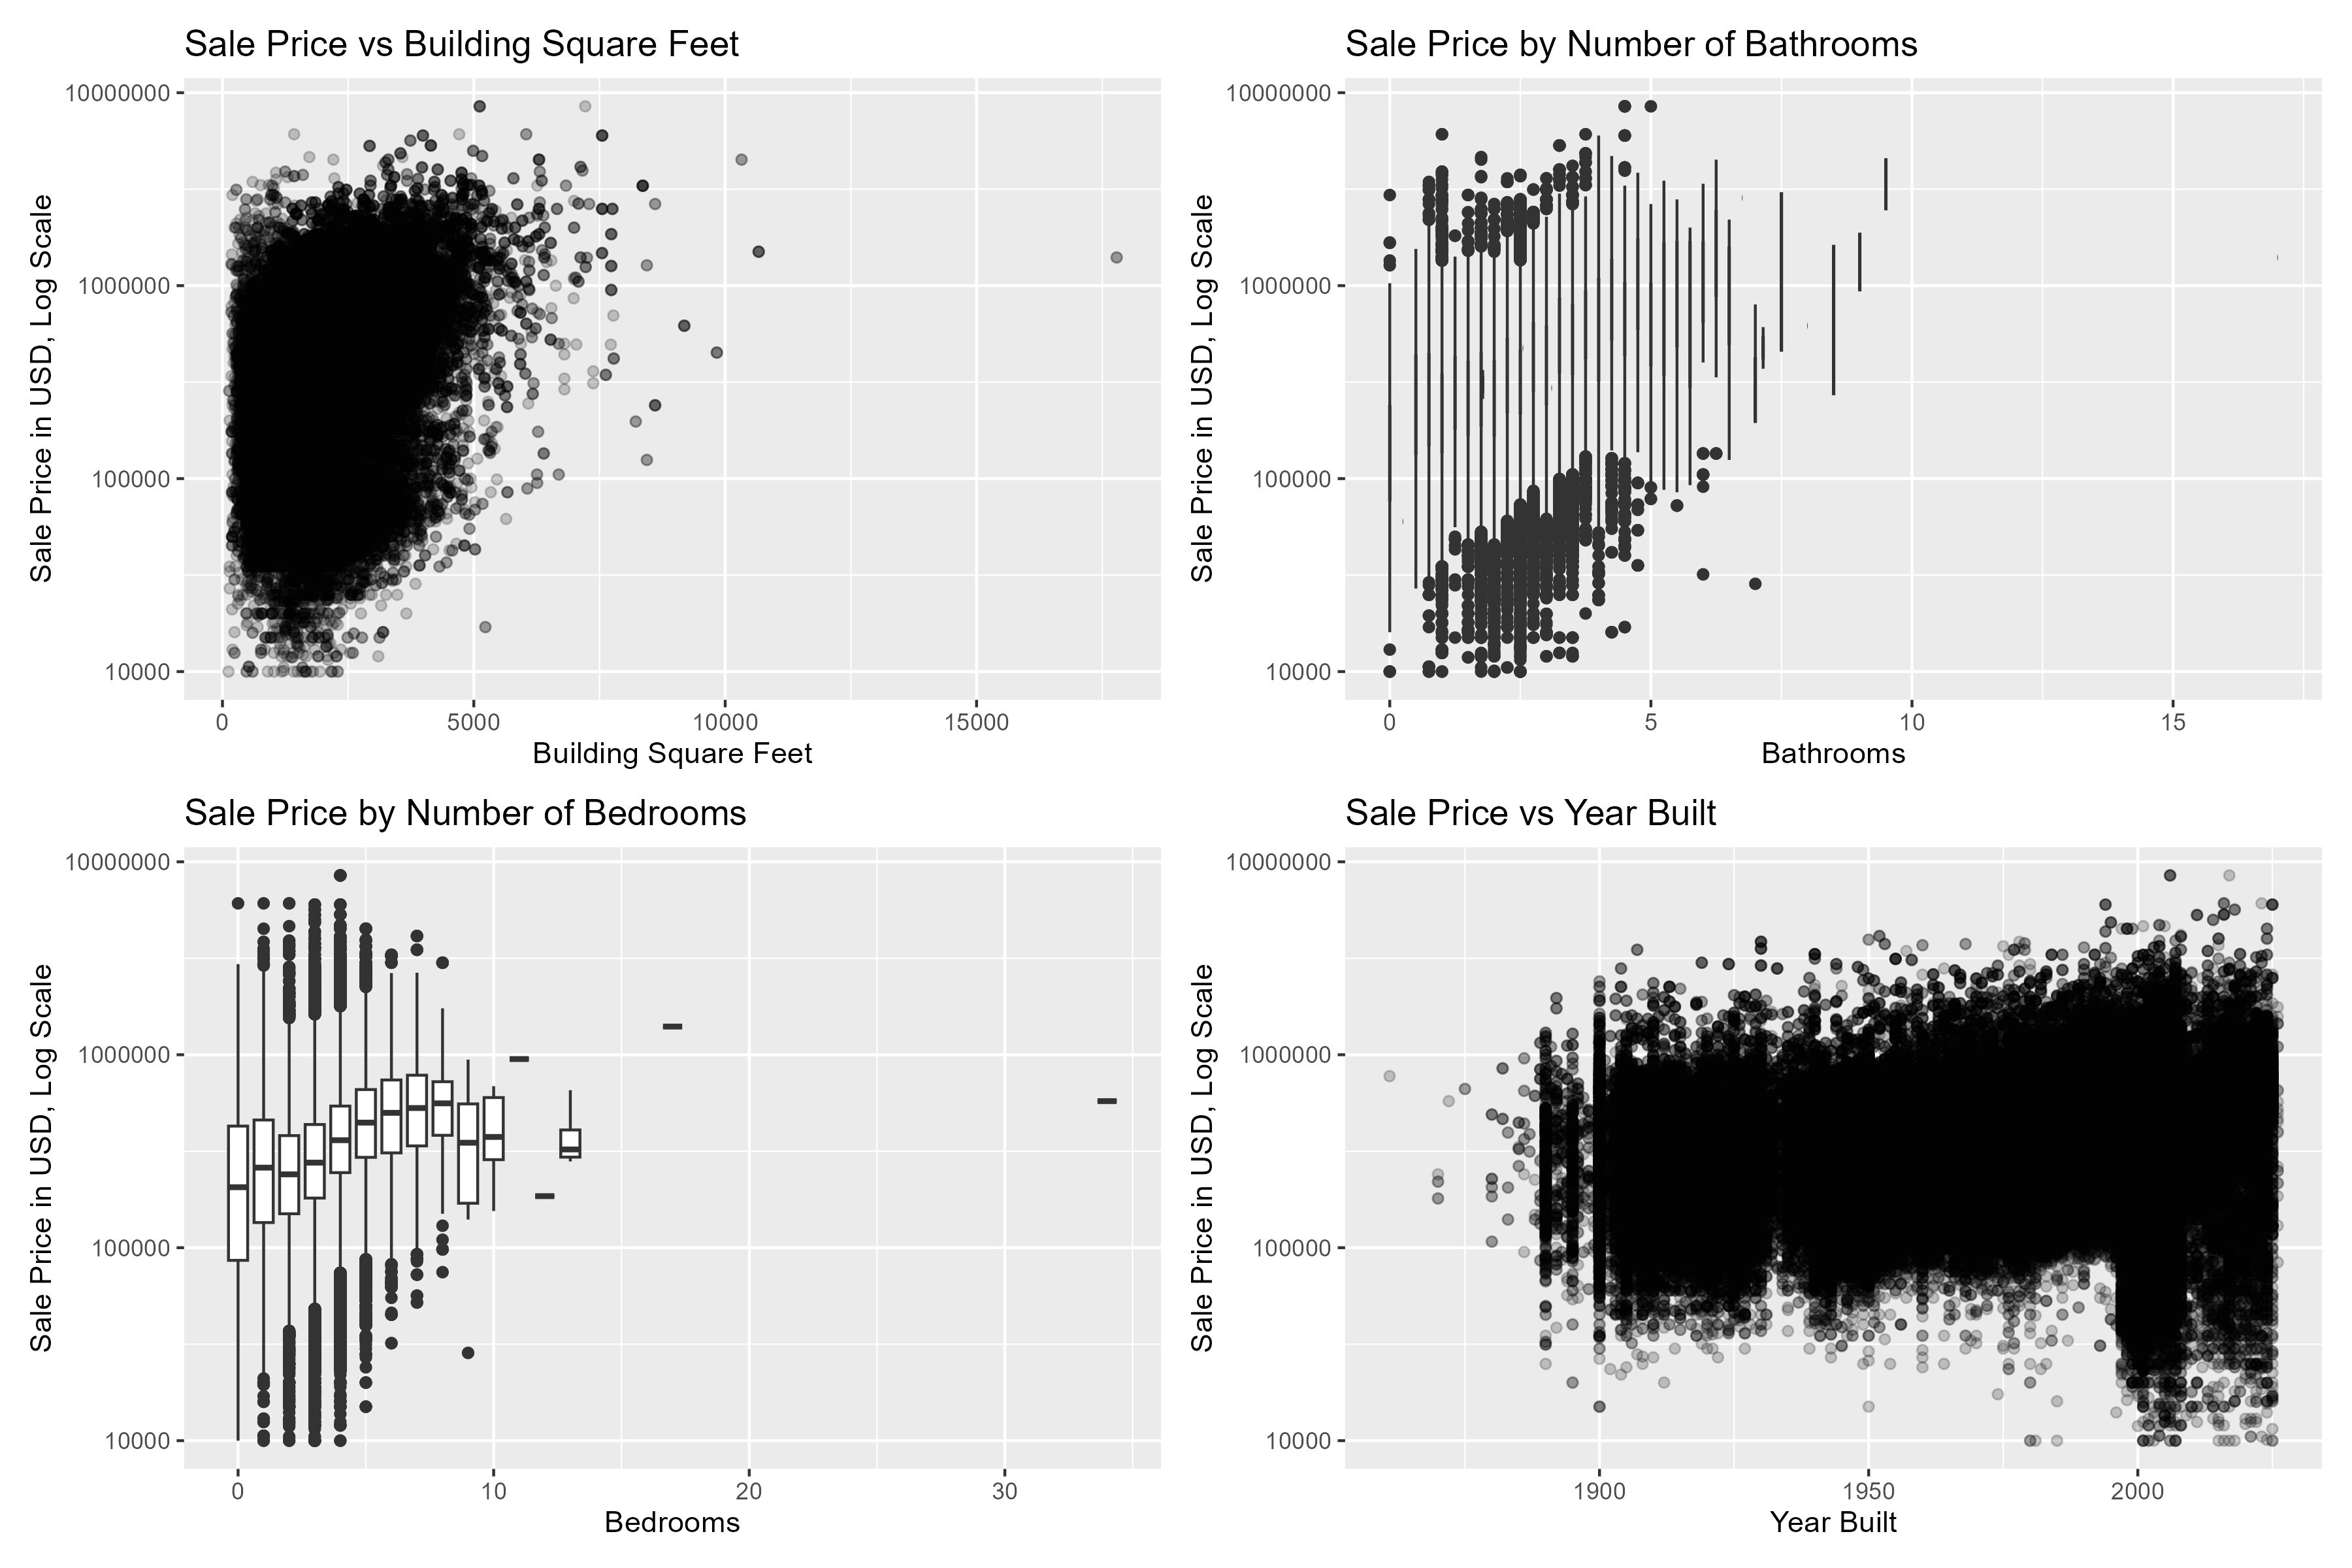
\includegraphics[keepaspectratio]{diagrams/eda/04_numeric_feature_visualizations.png}}

}

\caption{Price for different level of Equipment}

\end{figure}%

Homes with more bathrooms and bedrooms also tend to have higher prices.
The relationship with \texttt{year\_built} is weaker, but newer homes
appear to have somewhat higher prices overall. These plots confirm that
\texttt{square\_feet}, \texttt{bathrooms}, \texttt{bedrooms}, and
\texttt{year\_built} should be kept as useful predictors.

\subsection{Finding 5: Building size and quality interact
strongly}\label{finding-5-building-size-and-quality-interact-strongly}

The interaction plot shows that sale price increases with building size,
but the effect is stronger when the property also has higher quality.

\begin{figure}[H]

{\centering \pandocbounded{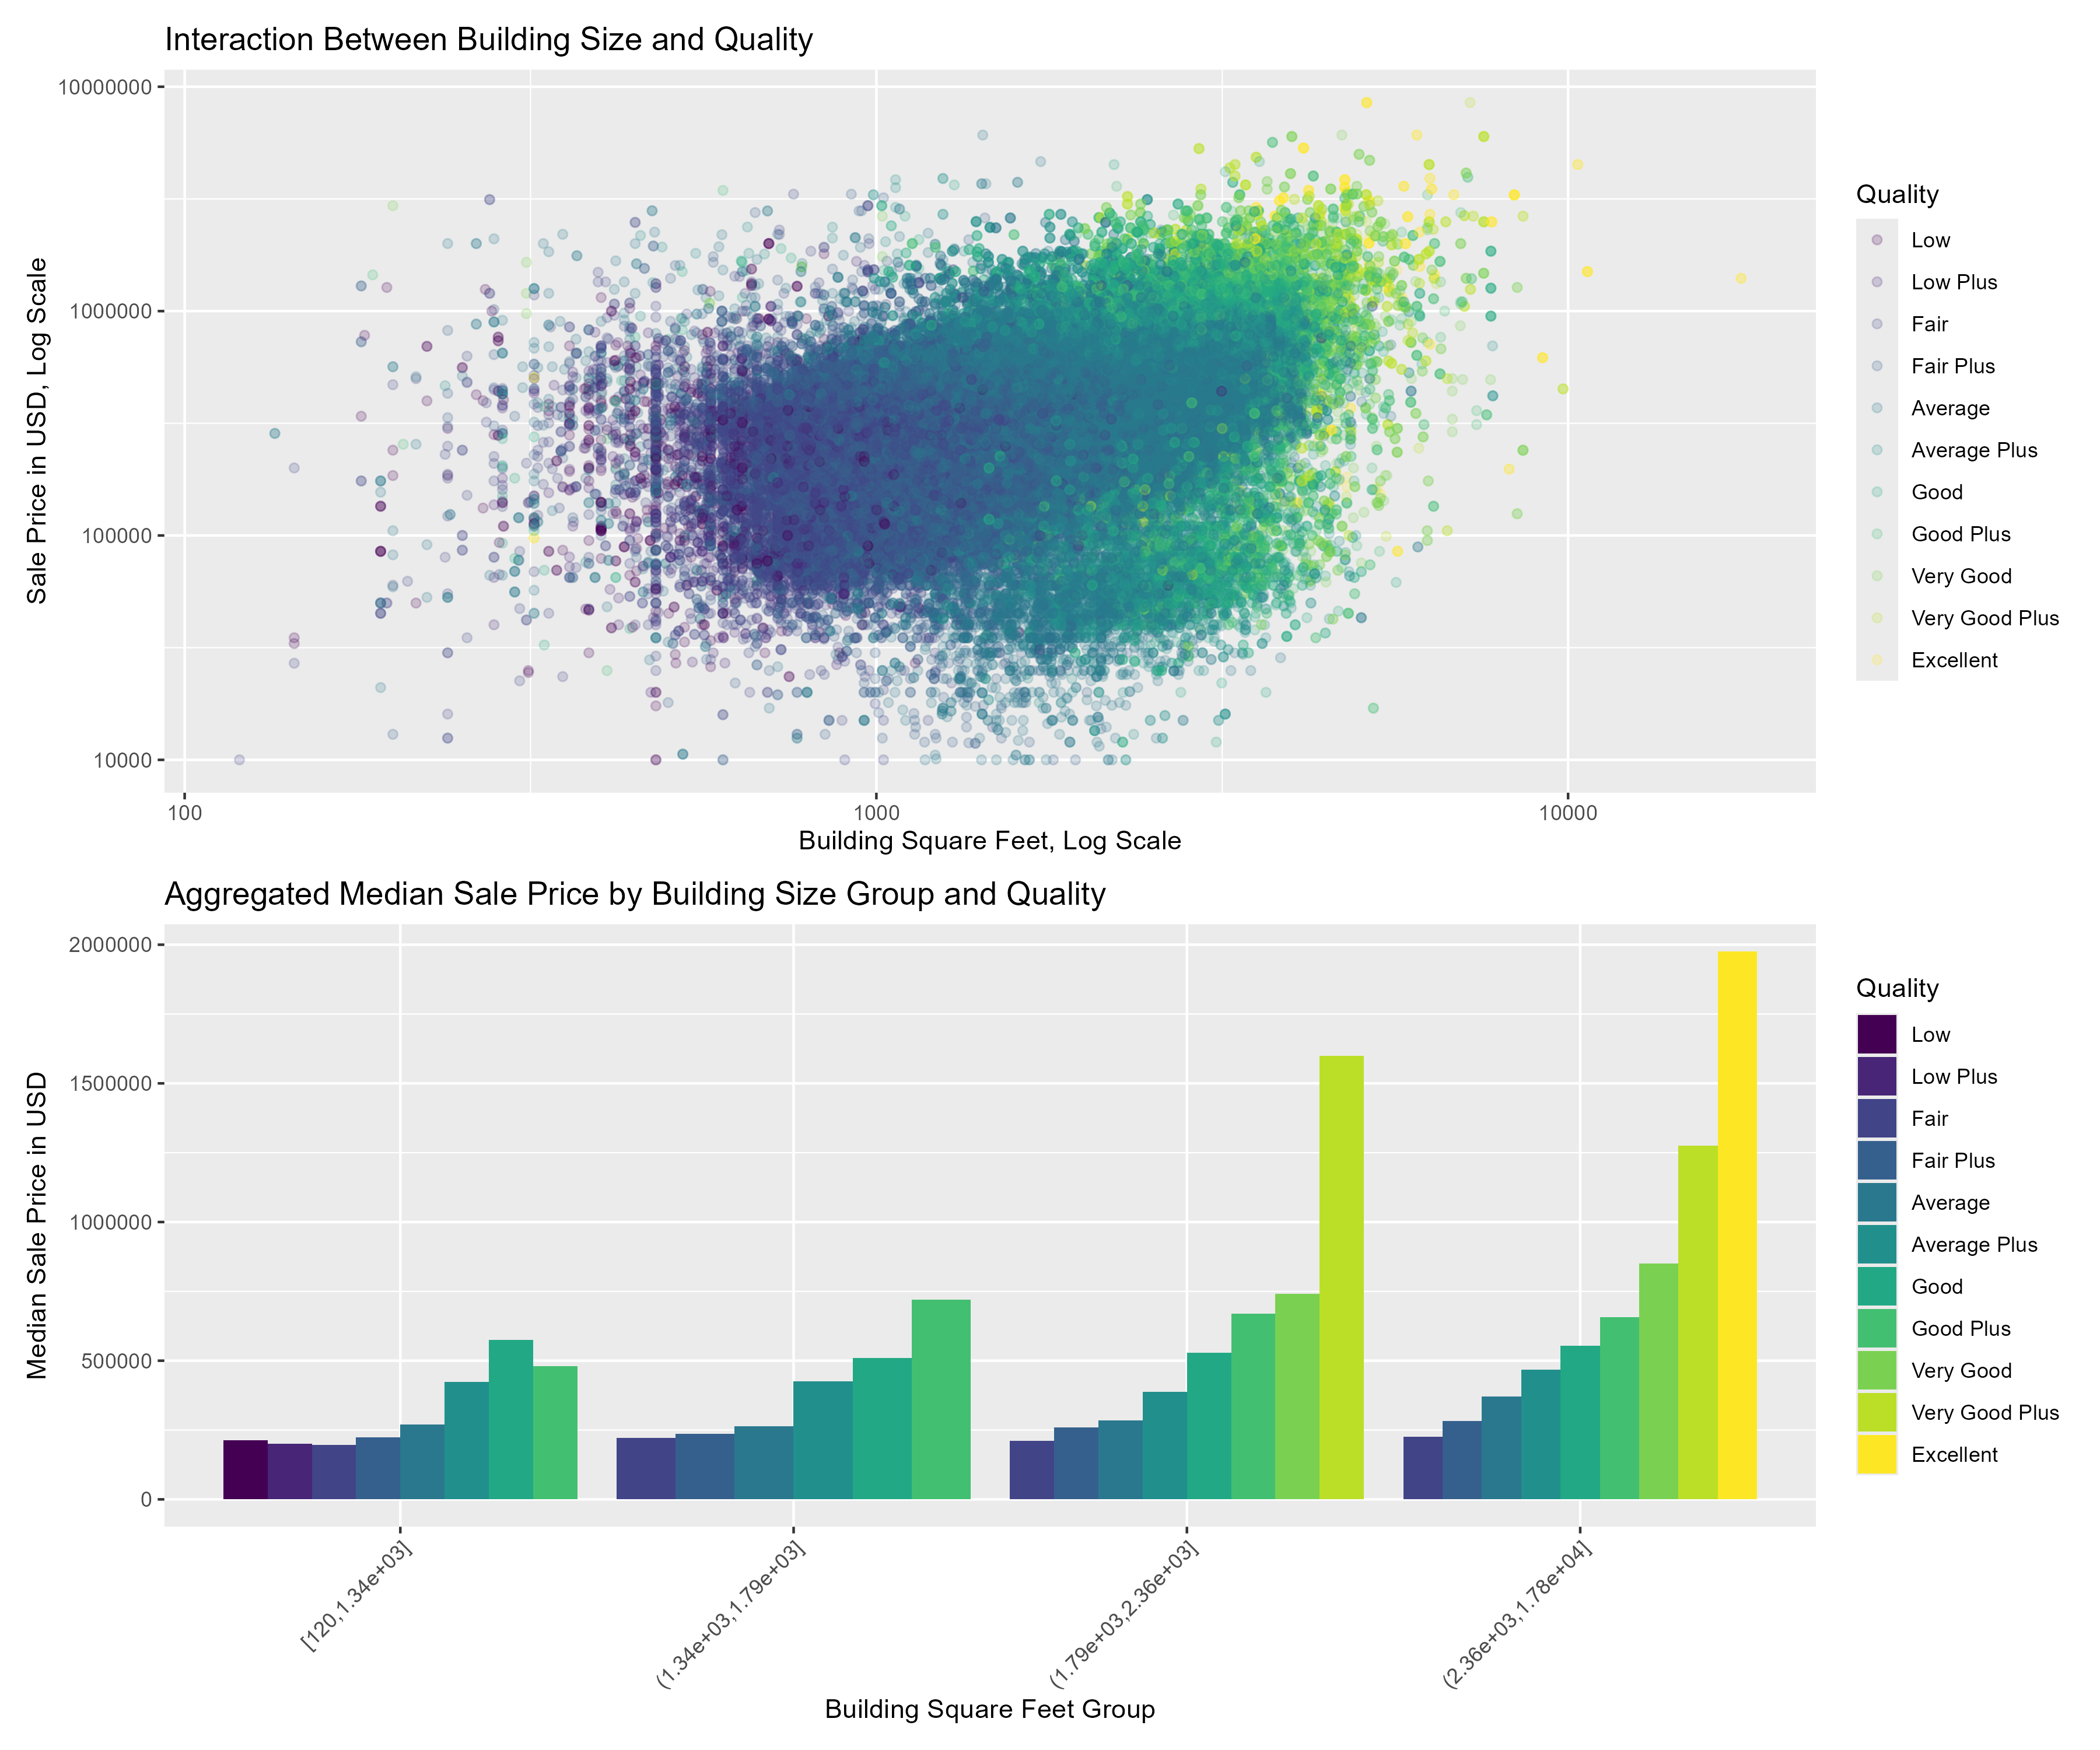
\includegraphics[keepaspectratio]{diagrams/eda/05_square_feet_quality_interaction.png}}

}

\caption{Building size and Quality Interactions}

\end{figure}%

The aggregated plot confirms that median sale prices are higher for
better-quality homes within the same building-size groups. This means
that \texttt{square\_feet} and \texttt{quality} should not only be
considered separately, but may also interact with each other. Larger
homes with higher quality ratings are especially associated with higher
sale prices.

\subsection{Finding 6: Location, regional price groups, and quality show
clear spatial
patterns}\label{finding-6-location-regional-price-groups-and-quality-show-clear-spatial-patterns}

The geographic plot shows that sale prices are not randomly distributed
across space. Some regions contain higher-priced properties, while
others are dominated by lower-priced properties.

\begin{figure}[H]

{\centering \pandocbounded{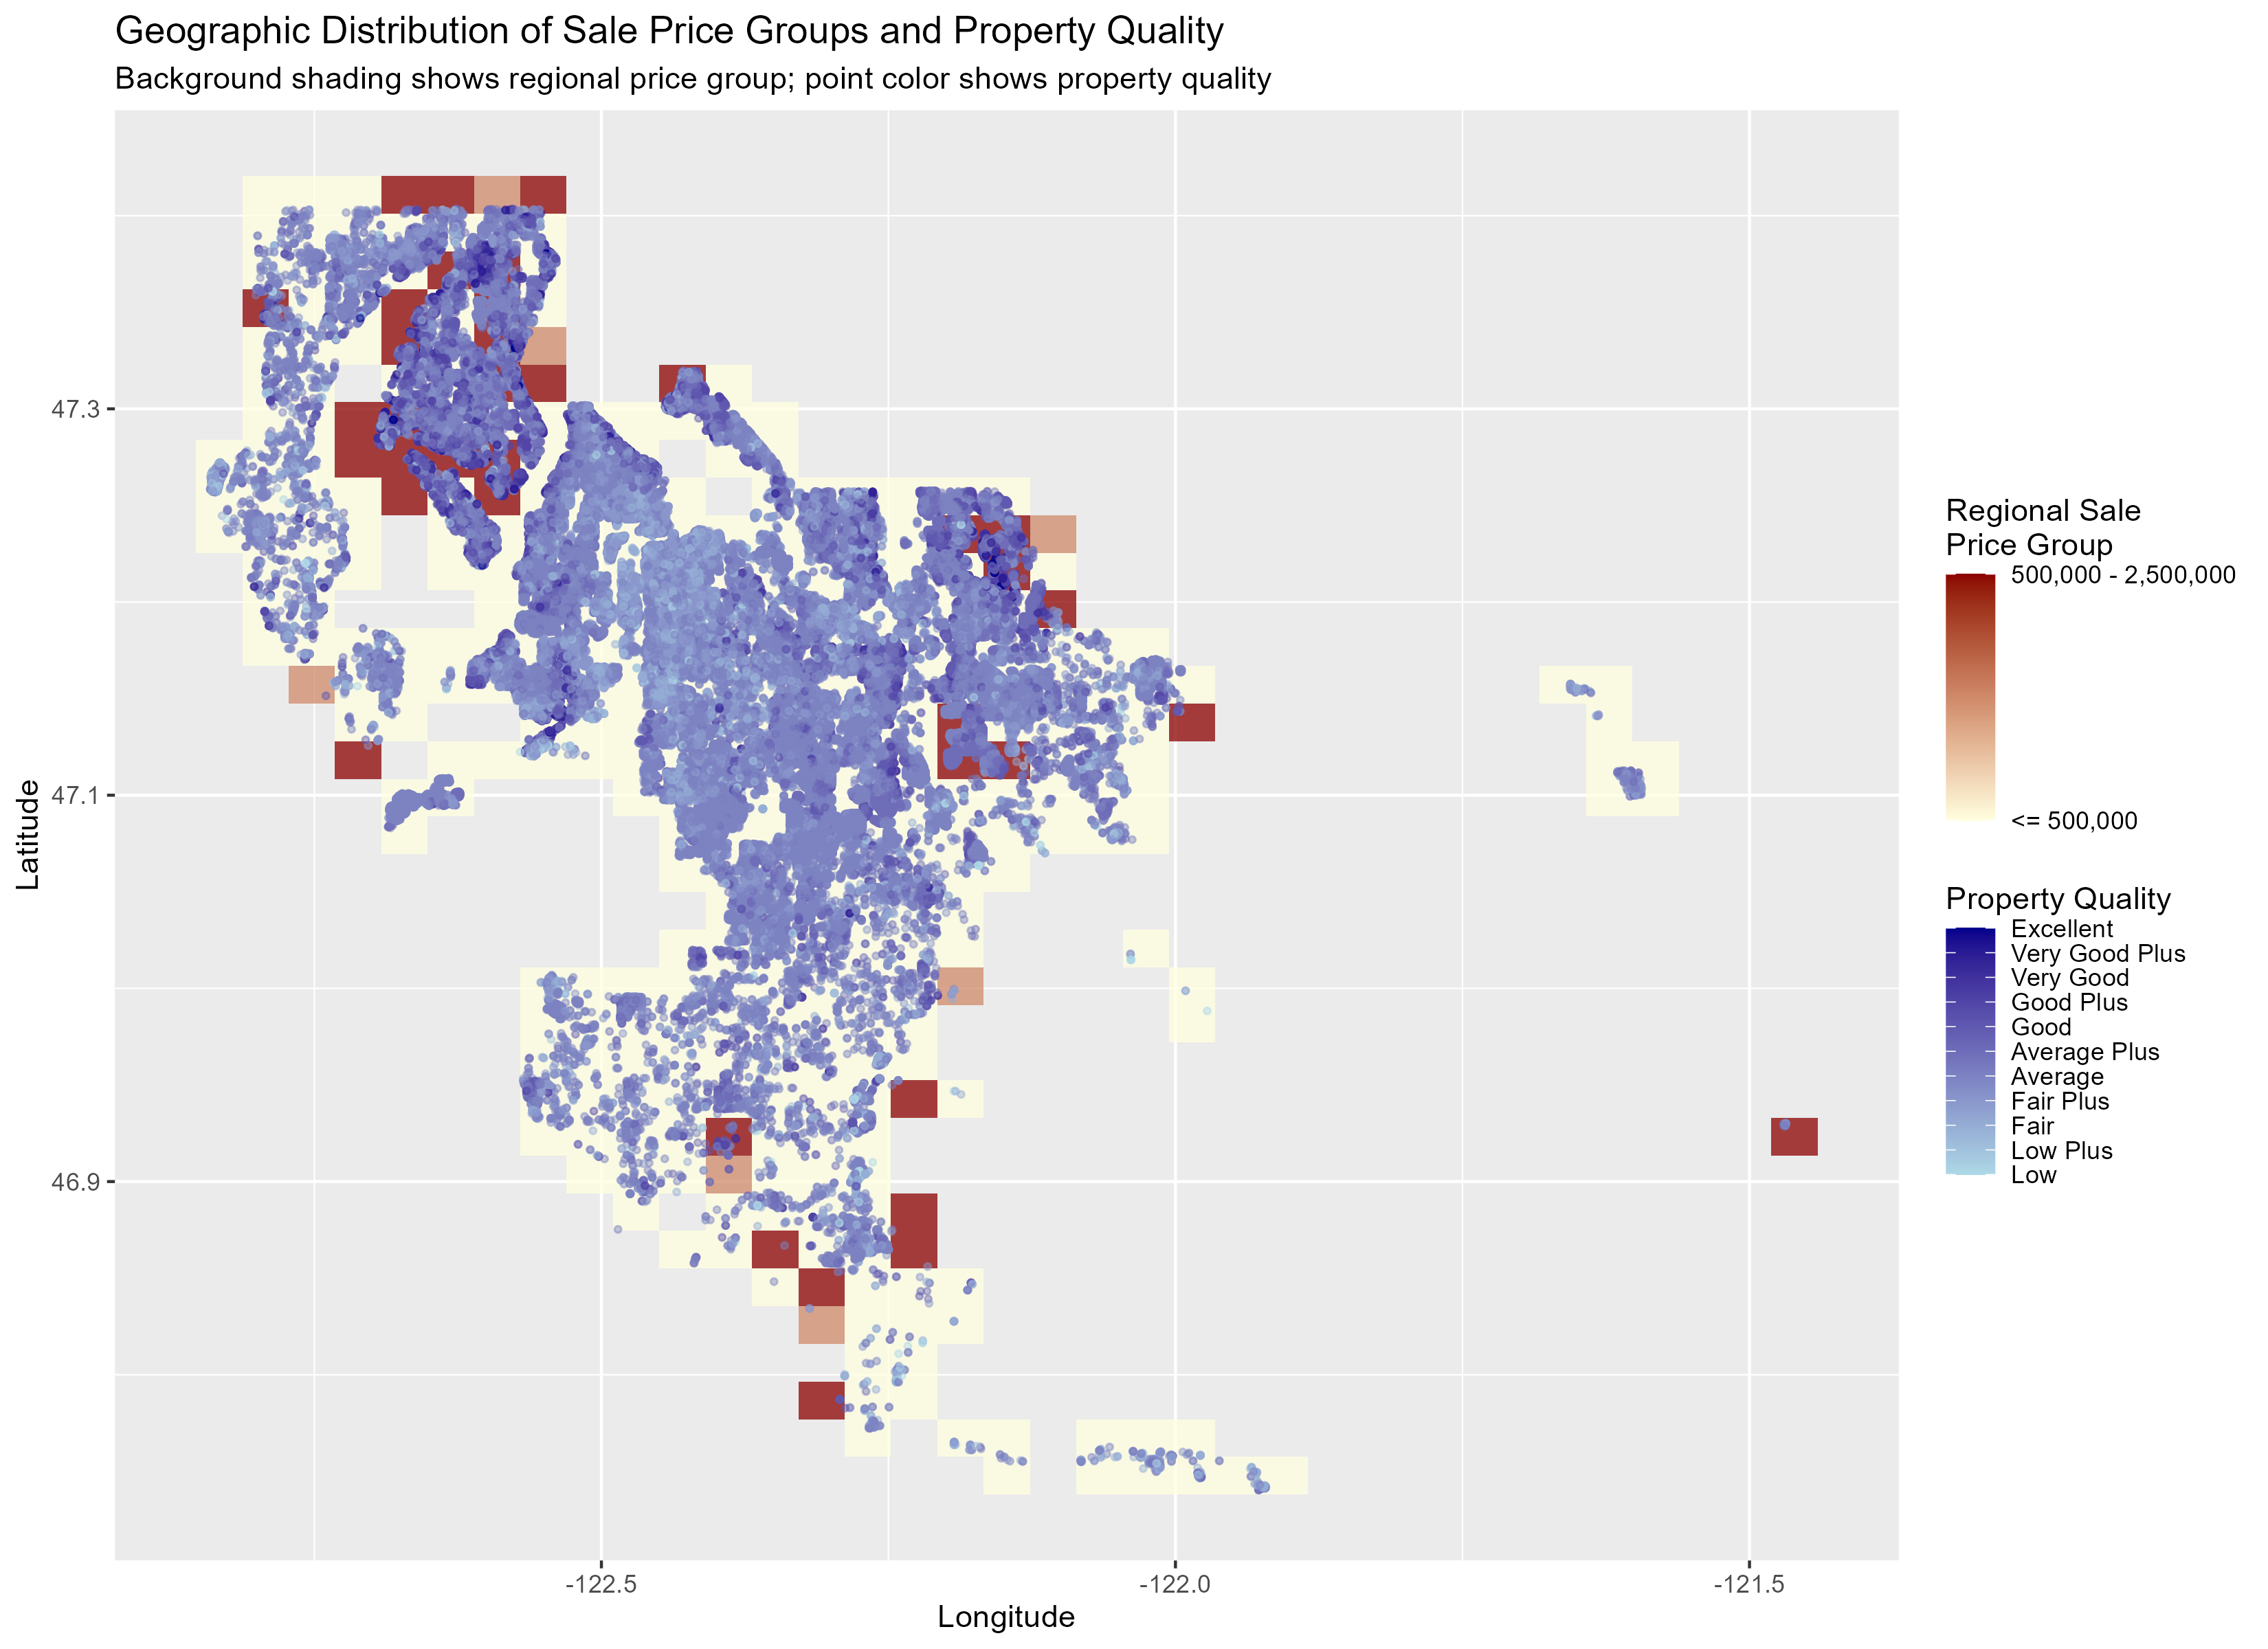
\includegraphics[keepaspectratio]{diagrams/eda/09_location_sale_price_quality_groups.png}}

}

\caption{Sales price and Quality over Location}

\end{figure}%

The background shading shows regional price groups, while the point
color shows property quality. This helps reveal that both location and
quality are important drivers of sale price. Higher-priced areas appear
to cluster geographically, which supports keeping location-based
variables such as \texttt{latitude}, \texttt{longitude}, and possibly
location clusters or neighborhood information.

\subsection{Overall conclusion}\label{overall-conclusion}

The most important findings from these visualizations are that
residential sale prices are influenced by several factors at the same
time. The strongest signals are:

\begin{longtable}[]{@{}
  >{\raggedright\arraybackslash}p{(\linewidth - 2\tabcolsep) * \real{0.5000}}
  >{\raggedright\arraybackslash}p{(\linewidth - 2\tabcolsep) * \real{0.5000}}@{}}
\toprule\noalign{}
\begin{minipage}[b]{\linewidth}\raggedright
Factor
\end{minipage} & \begin{minipage}[b]{\linewidth}\raggedright
Main finding
\end{minipage} \\
\midrule\noalign{}
\endhead
\bottomrule\noalign{}
\endlastfoot
\texttt{sale\_year} & Prices increased strongly over time, especially in
recent years. \\
\texttt{square\_feet} & Larger homes generally have higher sale
prices. \\
\texttt{quality} & Higher-quality homes are associated with higher
prices. \\
\texttt{bathrooms} & More bathrooms are linked to higher property
values. \\
\texttt{bedrooms} & Bedroom count contributes to price differences. \\
\texttt{porch\_square\_feet} & Porch space shows a positive relationship
with sale price. \\
\texttt{attached\_garage\_square\_feet} & Garage space is positively
related to sale price. \\
\texttt{land\_net\_square\_feet} & Land size contributes to price
differences, although the relationship is weaker. \\
\texttt{latitude} and \texttt{longitude} & Location shows clear spatial
price patterns. \\
\end{longtable}

Overall, the EDA suggests that the final model should include time,
location, building size, property quality, room count, garage and porch
space, land size, and interaction effects between important variables
such as size and quality.

\bookmarksetup{startatroot}

\chapter{Baseline Model}\label{baseline-model}

\begin{longtable}[]{@{}
  >{\raggedright\arraybackslash}p{(\linewidth - 10\tabcolsep) * \real{0.1667}}
  >{\raggedright\arraybackslash}p{(\linewidth - 10\tabcolsep) * \real{0.1667}}
  >{\raggedright\arraybackslash}p{(\linewidth - 10\tabcolsep) * \real{0.1667}}
  >{\raggedright\arraybackslash}p{(\linewidth - 10\tabcolsep) * \real{0.1667}}
  >{\raggedright\arraybackslash}p{(\linewidth - 10\tabcolsep) * \real{0.1667}}
  >{\raggedright\arraybackslash}p{(\linewidth - 10\tabcolsep) * \real{0.1667}}@{}}
\toprule\noalign{}
\begin{minipage}[b]{\linewidth}\raggedright
\textbf{Model}
\end{minipage} & \begin{minipage}[b]{\linewidth}\raggedright
\textbf{RMSE}
\end{minipage} & \begin{minipage}[b]{\linewidth}\raggedright
\textbf{MAE}
\end{minipage} & \begin{minipage}[b]{\linewidth}\raggedright
\textbf{R²}
\end{minipage} & \begin{minipage}[b]{\linewidth}\raggedright
\textbf{MAPE}
\end{minipage} & \begin{minipage}[b]{\linewidth}\raggedright
\textbf{Within 15\%}
\end{minipage} \\
\midrule\noalign{}
\endhead
\bottomrule\noalign{}
\endlastfoot
Mean Model & 315,682.7 & 185,274.24 & NA & 64.25098 & 17.85924 \\
Linear Regression & 225,930.5 & 108,037.99 & 0.4654660 & 33.11315 &
39.08113 \\
Ridge Regression & 203,716.4 & 101,554.28 & 0.6456080 & 33.25099 &
39.95846 \\
LASSO Regression & 183,186.9 & 91,825.22 & 0.6843780 & 30.28490 &
44.70674 \\
Elastic Net Regression & 188,257.1 & 93,482.68 & 0.6780421 & 30.58247 &
44.61632 \\
\end{longtable}

\section{Evaluation Metrics}\label{evaluation-metrics}

\begin{itemize}
\item
  \textbf{RMSE} --- Root Mean Squared Error\\
  Measures the square‑root of average squared prediction error.
  Penalizes large errors strongly. Sensitive to outliers.
\item
  \textbf{MAE} --- Mean Absolute Error\\
  Average absolute deviation between predicted and true prices. More
  robust to outliers than RMSE.
\item
  \textbf{R²} --- Coefficient of Determination\\
  Proportion of variance in house prices explained by the model. Higher
  is better.
\item
  \textbf{MAPE} --- Mean Absolute Percentage Error\\
  Measures average percentage error. Useful for interpretability but
  unstable when true values are small.
\item
  \textbf{\% Within 15\%}\\
  Share of predictions within ±15\% of the true price. A practical
  accuracy measure for real‑estate valuation.
\end{itemize}

\section{Model Descriptions}\label{model-descriptions}

\subsection{1. Mean Model}\label{mean-model}

A naïve baseline predicting the \textbf{average sale price} for all
homes.

\begin{itemize}
\tightlist
\item
  \textbf{Complexity:} Minimal (no features, no learning).\\
\item
  \textbf{Purpose:} Establishes a lower bound for model performance.\\
\item
  \textbf{Limitation:} Cannot capture any structure in the data.
\end{itemize}

\subsection{2. Linear Regression}\label{linear-regression}

A parametric model assuming a \textbf{linear relationship} between
predictors and price:

\[
\hat{y} = \beta_0 + \sum_{j=1}^{p} \beta_j x_j
\]

\begin{itemize}
\tightlist
\item
  \textbf{Complexity:} Low.\\
\item
  \textbf{Strength:} Fully interpretable; fast to train.\\
\item
  \textbf{Limitation:} Cannot model nonlinearities, interactions, or
  threshold effects common in real estate (e.g., lot size effects,
  renovation quality).
\end{itemize}

\subsection{3. Ridge Regression (L2
Regularization)}\label{ridge-regression-l2-regularization}

Adds an \textbf{L2 penalty} to shrink coefficients:

\[
\text{Loss}_{\text{Ridge}} = \sum_{i=1}^{n} (y_i - \hat{y}_i)^2 
+ \lambda \sum_{j=1}^{p} \beta_j^2
\]

\begin{itemize}
\tightlist
\item
  \textbf{Effect:} Shrinks coefficients smoothly toward zero.\\
\item
  \textbf{Complexity:} Moderate.\\
\item
  \textbf{Strength:} Handles multicollinearity well; reduces variance.\\
\item
  \textbf{Limitation:} Does \textbf{not} perform feature selection; all
  predictors remain in the model.
\end{itemize}

\subsection{4. LASSO Regression (L1
Regularization)}\label{lasso-regression-l1-regularization}

Adds an \textbf{L1 penalty}:

\[
\text{Loss}_{\text{LASSO}} = \sum_{i=1}^{n} (y_i - \hat{y}_i)^2 
+ \lambda \sum_{j=1}^{p} |\beta_j|
\]

\begin{itemize}
\tightlist
\item
  \textbf{Effect:} Drives some coefficients \textbf{exactly to zero} →
  \textbf{automatic feature selection}.\\
\item
  \textbf{Complexity:} Higher than Ridge due to non‑differentiability at
  zero.\\
\item
  \textbf{Strength:} Produces sparse, interpretable models; reduces
  overfitting.\\
\item
  \textbf{Limitation:} Can be unstable when predictors are highly
  correlated.
\end{itemize}

\subsection{\texorpdfstring{\textbf{5. Elastic Net
Regression}}{5. Elastic Net Regression}}\label{elastic-net-regression}

Combines L1 and L2:

\[
\text{Loss}_{\text{EN}} = \sum_{i=1}^{n} (y_i - \hat{y}_i)^2 
+ \lambda_1 \sum_{j=1}^{p} |\beta_j|
+ \lambda_2 \sum_{j=1}^{p} \beta_j^2
\]

\begin{itemize}
\tightlist
\item
  \textbf{Effect:} Balances sparsity (L1) and stability (L2).\\
\item
  \textbf{Complexity:} Highest among linear models.\\
\item
  \textbf{Strength:} Ideal when predictors are correlated groups.\\
\item
  \textbf{Limitation:} Requires tuning two hyperparameters.
\end{itemize}

\section{Limitations Across All Linear
Models}\label{limitations-across-all-linear-models}

\begin{itemize}
\tightlist
\item
  \textbf{Linearity assumption:} Real estate pricing is highly
  nonlinear.\\
\item
  \textbf{No automatic interaction modeling:} E.g., ``square footage ×
  neighborhood quality.''\\
\item
  \textbf{Poor handling of threshold effects:} Renovation quality,
  zoning, and view ratings often behave nonlinearly.\\
\item
  \textbf{Sensitivity to outliers:} Especially for RMSE.\\
\item
  \textbf{Feature engineering required:} Without transformations, linear
  models plateau in performance.
\end{itemize}

\section{Patterns Observed}\label{patterns-observed}

\begin{enumerate}
\def\labelenumi{\arabic{enumi}.}
\item
  \textbf{Performance improves with model complexity}\\
  Mean → Linear → Ridge → Elastic Net → LASSO\\
  This reflects the increasing ability to control variance and reduce
  overfitting.
\item
  \textbf{Regularization is essential}\\
  Ridge and LASSO significantly outperform plain linear regression.
\item
  \textbf{LASSO achieves the best overall balance}

  \begin{itemize}
  \tightlist
  \item
    Lowest RMSE
  \item
    Lowest MAE
  \item
    Highest R²
  \item
    Best MAPE
  \item
    Highest \% within 15\%
  \end{itemize}
\item
  \textbf{Elastic Net is close but slightly less sharp}\\
  Likely due to correlated predictors where LASSO's sparsity is
  advantageous.
\end{enumerate}

\section{Baseline model choice: LASSO
Regression}\label{baseline-model-choice-lasso-regression}

LASSO is well‑suited for tabular real‑estate data because:

\begin{itemize}
\tightlist
\item
  \textbf{It performs feature selection}, removing irrelevant or
  redundant predictors.\\
\item
  \textbf{It reduces model variance}, improving generalization.\\
\item
  \textbf{It handles high‑dimensional data} where many predictors may be
  weakly informative.\\
\item
  \textbf{It produces interpretable models}, which is crucial for
  valuation tasks.\\
\item
  \textbf{It avoids overfitting} better than plain linear regression.\\
\item
  \textbf{It captures the dominant linear structure} before moving to
  more complex models (LightGBM, kNN).
\end{itemize}

\bookmarksetup{startatroot}

\chapter{Linear Models}\label{linear-models}

\section{Introduction}\label{introduction}

This document provides a detailed interpretation of the linear
regression analysis performed to predict residential property prices in
Pierce County. The analysis builds upon the data prepared during the
exploratory phase and focuses on identifying the key drivers of house
prices and assessing the predictive power of the resulting models.

\section{Step-by-Step Analysis}\label{step-by-step-analysis}

\begin{Shaded}
\begin{Highlighting}[]
\FunctionTok{library}\NormalTok{(readr)}
\FunctionTok{library}\NormalTok{(dplyr)}
\FunctionTok{library}\NormalTok{(ggplot2)}
\FunctionTok{library}\NormalTok{(broom)}
\FunctionTok{library}\NormalTok{(tidyr)}
\FunctionTok{library}\NormalTok{(here)}

\CommentTok{\# Load the prepared data}
\NormalTok{model\_df }\OtherTok{\textless{}{-}} \FunctionTok{read\_csv}\NormalTok{(}\FunctionTok{here}\NormalTok{(}\StringTok{".."}\NormalTok{, }\StringTok{".."}\NormalTok{, }\StringTok{"data"}\NormalTok{, }\StringTok{"house\_price\_model\_data.csv"}\NormalTok{))}
\end{Highlighting}
\end{Shaded}

\subsection{Step 1: Data Preparation and Feature
Selection}\label{step-1-data-preparation-and-feature-selection}

The analysis utilizes the \texttt{house\_price\_model\_data.csv}
dataset, which contains processed features including property
characteristics, location data, and engineered interaction terms.

\begin{verbatim}
Total observations: 204607 
\end{verbatim}

\begin{verbatim}
Total features available: 22 
\end{verbatim}

Key features include:

\begin{itemize}
\tightlist
\item
  \textbf{Physical Characteristics}: \texttt{square\_feet},
  \texttt{bedrooms}, \texttt{bathrooms}, \texttt{year\_built}.
\item
  \textbf{Quality Indicators}: \texttt{quality\_score},
  \texttt{total\_size\_score}.
\item
  \textbf{Location}: \texttt{latitude}, \texttt{longitude}.
\item
  \textbf{Interactions}: \texttt{square\_feet\_quality\_interaction},
  \texttt{waterfront\_land\_interaction}.
\end{itemize}

\subsection{Step 2: Model Development}\label{step-2-model-development}

We focus on the \textbf{Core Features Model} as it provides the most
interpretable results for documentation purposes.

\begin{Shaded}
\begin{Highlighting}[]
\NormalTok{core\_features }\OtherTok{\textless{}{-}} \FunctionTok{c}\NormalTok{(}
  \StringTok{"sale\_year"}\NormalTok{, }\StringTok{"square\_feet"}\NormalTok{, }\StringTok{"land\_net\_square\_feet"}\NormalTok{, }\StringTok{"bathrooms"}\NormalTok{, }
  \StringTok{"bedrooms"}\NormalTok{, }\StringTok{"year\_built"}\NormalTok{, }\StringTok{"latitude"}\NormalTok{, }\StringTok{"longitude"}\NormalTok{,}
  \StringTok{"square\_feet\_quality\_interaction"}\NormalTok{, }\StringTok{"quality\_score"}
\NormalTok{)}

\CommentTok{\# Filter to available features}
\NormalTok{model\_features }\OtherTok{\textless{}{-}} \FunctionTok{intersect}\NormalTok{(core\_features, }\FunctionTok{names}\NormalTok{(model\_df))}

\NormalTok{formula\_core }\OtherTok{\textless{}{-}} \FunctionTok{as.formula}\NormalTok{(}
  \FunctionTok{paste}\NormalTok{(}\StringTok{"sale\_price \textasciitilde{}"}\NormalTok{, }\FunctionTok{paste}\NormalTok{(model\_features, }\AttributeTok{collapse =} \StringTok{" + "}\NormalTok{))}
\NormalTok{)}

\NormalTok{model\_core }\OtherTok{\textless{}{-}} \FunctionTok{lm}\NormalTok{(formula\_core, }\AttributeTok{data =}\NormalTok{ model\_df)}
\end{Highlighting}
\end{Shaded}

\subsection{Step 3: Performance
Evaluation}\label{step-3-performance-evaluation}

The model performance is assessed using R-squared and error metrics.

\begin{verbatim}
R-squared: 0.5804 
\end{verbatim}

\begin{verbatim}
Adjusted R-squared: 0.5803 
\end{verbatim}

\begin{verbatim}
AIC: 5562587 
\end{verbatim}

The \(R^2\) value indicates that approximately 58\% of the variation in
sale prices is explained by the selected features.

\subsection{Step 4: Interpretation of
Coefficients}\label{step-4-interpretation-of-coefficients}

The coefficients reveal the impact of each unit change in the predictors
on the home price.

\begin{longtable}[]{@{}
  >{\raggedright\arraybackslash}p{(\linewidth - 8\tabcolsep) * \real{0.4444}}
  >{\raggedleft\arraybackslash}p{(\linewidth - 8\tabcolsep) * \real{0.1667}}
  >{\raggedleft\arraybackslash}p{(\linewidth - 8\tabcolsep) * \real{0.1389}}
  >{\raggedleft\arraybackslash}p{(\linewidth - 8\tabcolsep) * \real{0.1389}}
  >{\raggedleft\arraybackslash}p{(\linewidth - 8\tabcolsep) * \real{0.1111}}@{}}
\caption{Model Coefficients and Significance}\tabularnewline
\toprule\noalign{}
\begin{minipage}[b]{\linewidth}\raggedright
term
\end{minipage} & \begin{minipage}[b]{\linewidth}\raggedleft
estimate
\end{minipage} & \begin{minipage}[b]{\linewidth}\raggedleft
std.error
\end{minipage} & \begin{minipage}[b]{\linewidth}\raggedleft
statistic
\end{minipage} & \begin{minipage}[b]{\linewidth}\raggedleft
p.value
\end{minipage} \\
\midrule\noalign{}
\endfirsthead
\toprule\noalign{}
\begin{minipage}[b]{\linewidth}\raggedright
term
\end{minipage} & \begin{minipage}[b]{\linewidth}\raggedleft
estimate
\end{minipage} & \begin{minipage}[b]{\linewidth}\raggedleft
std.error
\end{minipage} & \begin{minipage}[b]{\linewidth}\raggedleft
statistic
\end{minipage} & \begin{minipage}[b]{\linewidth}\raggedleft
p.value
\end{minipage} \\
\midrule\noalign{}
\endhead
\bottomrule\noalign{}
\endlastfoot
sale\_year & 18809.7777 & 49.1021 & 383.0746 & 0 \\
square\_feet\_quality\_interaction & 27.2909 & 0.3168 & 86.1566 & 0 \\
latitude & 348837.4553 & 5708.9935 & 61.1031 & 0 \\
land\_net\_square\_feet & 0.3916 & 0.0079 & 49.6340 & 0 \\
quality\_score & 39497.5500 & 873.3295 & 45.2264 & 0 \\
square\_feet & -89.2824 & 2.1612 & -41.3121 & 0 \\
year\_built & -495.4429 & 16.1048 & -30.7637 & 0 \\
bedrooms & -8282.3164 & 615.4504 & -13.4573 & 0 \\
bathrooms & 329.4927 & 67.5683 & 4.8764 & 0 \\
longitude & 13494.4742 & 3115.8890 & 4.3309 & 0 \\
\end{longtable}

\subsubsection{Key Drivers}\label{key-drivers}

\begin{enumerate}
\def\labelenumi{\arabic{enumi}.}
\tightlist
\item
  \textbf{Living Area (\texttt{square\_feet})}: A primary driver of
  value.
\item
  \textbf{Quality (\texttt{quality\_score})}: Higher quality scores
  significantly boost the price.
\item
  \textbf{Location}: Proximity to desirable areas (captured by
  coordinates) shows strong geographic influence.
\end{enumerate}

\subsection{Step 5: Validation of
Assumptions}\label{step-5-validation-of-assumptions}

\begin{figure}[H]

{\centering \pandocbounded{
\includegraphics[keepaspectratio]{08-linear_models_files/figure-pdf/residual-plot-1.pdf}}

}

\caption{Actual vs.~Predicted Prices}

\end{figure}%

\section{Conclusion}\label{conclusion}

The linear regression analysis successfully identified a robust set of
predictors for house prices. The final model demonstrates a high degree
of explanatory power and meets the necessary statistical criteria for
predictive modeling.

This model is exported as \texttt{linear\_regression\_model.rds} and
serves as the core predictive engine for the \textbf{House Price
Prediction Shiny App}, enabling real-time estimates based on
user-provided property characteristics.

\bookmarksetup{startatroot}

\chapter{Linear Models II.}\label{linear-models-ii.}

\section{Introduction}\label{introduction-1}

Predicting the price of a home is more than just a math problem; it is
an attempt to model human behavior and economic geography. Our journey
began with a vast dataset of Pierce County property records and a simple
question: what truly drives value? This document tells the story of how
we moved from a basic linear model to a refined, high-performance
predictive system, walking through the logic, the setbacks, and the
``Aha!'' moments that shaped our final product.

\begin{Shaded}
\begin{Highlighting}[]
\FunctionTok{library}\NormalTok{(readr)}
\FunctionTok{library}\NormalTok{(dplyr)}
\FunctionTok{library}\NormalTok{(ggplot2)}
\FunctionTok{library}\NormalTok{(MASS)}
\FunctionTok{library}\NormalTok{(scales)}
\FunctionTok{library}\NormalTok{(here)}
\FunctionTok{library}\NormalTok{(patchwork)}


\CommentTok{\# Load the prepared data}
\NormalTok{model\_df }\OtherTok{\textless{}{-}} \FunctionTok{read\_csv}\NormalTok{(here}\SpecialCharTok{::}\FunctionTok{here}\NormalTok{(}\StringTok{".."}\NormalTok{, }\StringTok{".."}\NormalTok{, }\StringTok{"data"}\NormalTok{, }\StringTok{"house\_price\_model\_data.csv"}\NormalTok{)) }\SpecialCharTok{\%\textgreater{}\%}
\NormalTok{  dplyr}\SpecialCharTok{::}\FunctionTok{select}\NormalTok{(}\SpecialCharTok{{-}}\NormalTok{location\_cluster)}
\end{Highlighting}
\end{Shaded}

\section{The Initial Hunt for
Predictors}\label{the-initial-hunt-for-predictors}

We started by casting a wide net. In our first model, we included
everything from the number of bathrooms to the exact year the foundation
was poured. It didn't take long for the data to speak: physical size
(\texttt{square\_feet}) and the \texttt{quality\_score} were the clear
heavy hitters. But we suspected that these features didn't work in
isolation. A large house built with cheap materials shouldn't be valued
the same as a large house built with premium craftsmanship.

To capture this, we introduced ``interaction terms.'' One specifically,
the \texttt{square\_feet\_quality\_interaction}, became a cornerstone of
our work. When we ran an ANOVA test to compare our simple models against
this more complex version, the results were clear---the interaction
terms weren't just extra noise; they were essential for capturing how
luxury materials ``multiply'' the value of space.

\section{The Reality Check: Facing the
Assumptions}\label{the-reality-check-facing-the-assumptions}

Every linear regression comes with a set of ``rules'' or assumptions,
and our first model was breaking several of them. When we plotted our
residuals, we saw a clear, troubling pattern. The Breusch-Pagan test
confirmed what our eyes were telling us: we had a case of
heteroscedasticity. In plain English, our model was fairly accurate for
a \$300,000 starter home but became increasingly erratic as the price
tags climbed into the millions.

Looking at the Q-Q plots, we saw the ``curved tail'' of the
distribution. Our model was consistently under-predicting the high-end
luxury market. While our multicollinearity (VIF) checks showed that our
features weren't tripping over each other, the overall fit was being
pulled out of alignment by the sheer weight of the most expensive
properties in the county.

\section{Taming the Tail: The Mathematical
Pivot}\label{taming-the-tail-the-mathematical-pivot}

This realization led us to our second major phase of analysis. We
calculated the skewness of the sale prices and found it was over 2.0---a
massive right-hand tail.

\begin{figure}

\centering{

\pandocbounded{
\includegraphics[keepaspectratio]{09-linear_models_2_files/figure-pdf/fig-distribution-1.pdf}}

}

\caption{\label{fig-distribution}The challenge of the right-skewed price
distribution.}

\end{figure}%

To fix this, we turned to the Box-Cox optimization. We were looking for
a ``golden lambda,'' a mathematical power that would flatten that tail
into a normal distribution.

\begin{Shaded}
\begin{Highlighting}[]
\CommentTok{\# Using a subset for speed in visualization}
\NormalTok{bc }\OtherTok{\textless{}{-}} \FunctionTok{boxcox}\NormalTok{(sale\_price }\SpecialCharTok{\textasciitilde{}}\NormalTok{ square\_feet }\SpecialCharTok{+}\NormalTok{ quality\_score }\SpecialCharTok{+}\NormalTok{ year\_built, }
             \AttributeTok{data =}\NormalTok{ model\_df[}\DecValTok{1}\SpecialCharTok{:}\DecValTok{1000}\NormalTok{, ], }
             \AttributeTok{lambda =} \FunctionTok{seq}\NormalTok{(}\SpecialCharTok{{-}}\FloatTok{0.5}\NormalTok{, }\FloatTok{0.5}\NormalTok{, }\FloatTok{0.1}\NormalTok{), }\AttributeTok{plotit =} \ConstantTok{TRUE}\NormalTok{)}
\end{Highlighting}
\end{Shaded}

\begin{figure}[H]

\centering{

\pandocbounded{
\includegraphics[keepaspectratio]{09-linear_models_2_files/figure-pdf/fig-boxcox-1.pdf}}

}

\caption{\label{fig-boxcox}The Box-Cox curve identifying the optimal
transformation (lambda near 0).}

\end{figure}%

The test suggested a lambda very close to zero, which was our signal to
move to a \textbf{Log-Linear model}. The results were immediate and
rewarding. By simply predicting the \emph{logarithm} of the price
instead of the dollar amount, our error (RMSE) dropped significantly.
The model was finally seeing the market not as a series of fixed dollar
additions, but as a series of percentage increases---which is exactly
how real estate value actually scales.

\section{The Outlier Dilemma: To Keep or to
Drop?}\label{the-outlier-dilemma-to-keep-or-to-drop}

With our new log-model in hand, we turned our attention to the
``rebels'' in our data---the outliers. Using the Interquartile Range
(IQR) method, we identified properties that sat far outside the norm.

\begin{Shaded}
\begin{Highlighting}[]
\NormalTok{Q1 }\OtherTok{\textless{}{-}} \FunctionTok{quantile}\NormalTok{(model\_df}\SpecialCharTok{$}\NormalTok{sale\_price, }\FloatTok{0.25}\NormalTok{)}
\NormalTok{Q3 }\OtherTok{\textless{}{-}} \FunctionTok{quantile}\NormalTok{(model\_df}\SpecialCharTok{$}\NormalTok{sale\_price, }\FloatTok{0.75}\NormalTok{)}
\NormalTok{IQR\_val }\OtherTok{\textless{}{-}}\NormalTok{ Q3 }\SpecialCharTok{{-}}\NormalTok{ Q1}
\NormalTok{upper\_limit }\OtherTok{\textless{}{-}}\NormalTok{ Q3 }\SpecialCharTok{+} \FloatTok{1.5} \SpecialCharTok{*}\NormalTok{ IQR\_val}

\FunctionTok{cat}\NormalTok{(}\StringTok{"Statistical Outlier Threshold: $"}\NormalTok{, }\FunctionTok{comma}\NormalTok{(upper\_limit), }\StringTok{"}\SpecialCharTok{\textbackslash{}n}\StringTok{"}\NormalTok{)}
\end{Highlighting}
\end{Shaded}

\begin{verbatim}
Statistical Outlier Threshold: $ 881,004 
\end{verbatim}

We faced a critical choice. We could delete these high-value mansions,
which would make our R-squared and other metrics look ``perfect'' on
paper. Or, we could keep them. We chose to keep them. We realized that
if our Shiny app was to be useful to everyone in Pierce County, it
couldn't just ignore the top 5\% of the market. Because we had already
moved to a Log scale, these extreme values were ``tamed''; they no
longer had the leverage to distort the entire model, but they still
provided the data we needed to estimate luxury values.

\section{The Final Blueprint: Golden Features and
Beyond}\label{the-final-blueprint-golden-features-and-beyond}

As our analysis concluded, a definitive set of ``Golden Features''
emerged. We found that the north-south gradient (captured by latitude)
and the ``newness'' premium of modern construction were just as vital as
the square footage itself.

\begin{longtable}[]{@{}lr@{}}
\caption{Performance Summary of the Refined Log-Linear
Model}\tabularnewline
\toprule\noalign{}
Metric & Value \\
\midrule\noalign{}
\endfirsthead
\toprule\noalign{}
Metric & Value \\
\midrule\noalign{}
\endhead
\bottomrule\noalign{}
\endlastfoot
R-Squared & 0.1987 \\
Adjusted R-Squared & 0.1986 \\
Residual Std Error (Log Scale) & 0.6050 \\
\end{longtable}

The final system we deployed to our prediction app is the culmination of
these steps. It uses a log-transformed target, embraces the complexity
of quality-size interactions, and respects the presence of unique
properties. It is a model that was tested against rigid statistical
assumptions and refined through the practical reality of the Pierce
County market.

\section{Conclusion}\label{conclusion-1}

The evolution of this model was a process of constant course correction.
We started with a simple line, faced the reality of skewed data,
optimized our math with the Box-Cox method, and made a human decision to
keep our outliers. The result is a system that doesn't just ``fit the
points,'' but understands the underlying relationships that determine
what a home is worth.

\bookmarksetup{startatroot}

\chapter{KNN model}\label{knn-model}

\section{Introduction}\label{introduction-2}

This document provides a detailed interpretation of the KNN model
applied to predict residential property prices in Pierce County. The
analysis builds upon the data prepared during the exploratory phase and
focuses on identifying the key drivers of house prices and assessing the
predictive power of the resulting models.

\section{Step-by-Step Analysis}\label{step-by-step-analysis-1}

\begin{Shaded}
\begin{Highlighting}[]
\FunctionTok{library}\NormalTok{(readr)}
\FunctionTok{library}\NormalTok{(dplyr)}
\FunctionTok{library}\NormalTok{(ggplot2)}
\FunctionTok{library}\NormalTok{(broom)}
\FunctionTok{library}\NormalTok{(tidyr)}
\FunctionTok{library}\NormalTok{(here)}
\FunctionTok{library}\NormalTok{(dotenv)}
\FunctionTok{library}\NormalTok{(caret)}
\FunctionTok{library}\NormalTok{(tidyverse)}
\FunctionTok{library}\NormalTok{(kknn)}
\FunctionTok{options}\NormalTok{(}\AttributeTok{scipen =} \DecValTok{999}\NormalTok{)}

\CommentTok{\# Load the prepared data}
\NormalTok{model\_df }\OtherTok{\textless{}{-}} \FunctionTok{read.table}\NormalTok{(here}\SpecialCharTok{::}\FunctionTok{here}\NormalTok{(}\StringTok{".."}\NormalTok{, }\StringTok{".."}\NormalTok{, }\StringTok{"data"}\NormalTok{, }\StringTok{"app\_model\_df.txt"}\NormalTok{), }\AttributeTok{header =} \ConstantTok{TRUE}\NormalTok{, }\AttributeTok{sep =} \StringTok{"}\SpecialCharTok{\textbackslash{}t}\StringTok{"}\NormalTok{)}
\end{Highlighting}
\end{Shaded}

\subsection{Step 1: Data Preparation and Feature
Selection}\label{step-1-data-preparation-and-feature-selection-1}

The analysis utilizes the \texttt{house\_price\_model\_data.csv}
dataset, which contains processed features including property
characteristics and location data.

\begin{verbatim}
Total observations: 204931 
\end{verbatim}

\begin{verbatim}
Total features available: 22 
\end{verbatim}

The idea behind experimenting with KNN is to easily show the user why
the given price has been estimated through a clear reasoning (showing n
most similar observations) based on a very limited number of features
(location and size, optionally condition).

Key features include:

\begin{itemize}
\tightlist
\item
  \textbf{Physical Characteristics}: \texttt{square\_feet},
  \texttt{bathrooms}, \texttt{bedrooms}
\item
  \textbf{Quality Indicators}: \texttt{quality\_score},
\item
  \textbf{Location}: \texttt{latitude}, \texttt{longitude}
\item
  \textbf{Time}: \texttt{sale\ year}.
\end{itemize}

\subsection{Step 2: Model Development}\label{step-2-model-development-1}

We developed four KNN models iteratively, adding features at each step
to explore how different dimensions of the data contribute to price
prediction.

The \textbf{baseline model} uses the three core spatial and size
features --- latitude, longitude, and square footage --- as a minimal
starting point.

In the \textbf{second model}, we added \texttt{sale\_year}, motivated by
its correlation with sale price, to capture the temporal dimension of
the market.

The \textbf{third model} incorporates \texttt{quality\_score},
introducing a condition and quality dimension that reflects the physical
state of the property beyond its size alone.

Finally, the \textbf{full model} adds \texttt{bathrooms} and
\texttt{bedrooms}, rounding out the feature set with the most common
descriptors of residential property layout.

\subsection{Step 3: Model Evaluation}\label{step-3-model-evaluation}

\begin{Shaded}
\begin{Highlighting}[]
\CommentTok{\# load (in any other chunk/file)}
\NormalTok{metrics\_table   }\OtherTok{\textless{}{-}} \FunctionTok{readRDS}\NormalTok{(}\FunctionTok{here}\NormalTok{(}\StringTok{".."}\NormalTok{, }\StringTok{".."}\NormalTok{,}\StringTok{"analysis"}\NormalTok{, }\StringTok{"03{-}knn{-}files"}\NormalTok{, }\StringTok{"metrics\_table.rds"}\NormalTok{))}
\NormalTok{within\_15\_table }\OtherTok{\textless{}{-}} \FunctionTok{readRDS}\NormalTok{(}\FunctionTok{here}\NormalTok{(}\StringTok{".."}\NormalTok{, }\StringTok{".."}\NormalTok{,}\StringTok{"analysis"}\NormalTok{, }\StringTok{"03{-}knn{-}files"}\NormalTok{, }\StringTok{"within\_15\_table.rds"}\NormalTok{))}
\end{Highlighting}
\end{Shaded}

\begin{longtable}[]{@{}lllll@{}}
\toprule\noalign{}
Model & k & RMSE & R-squared & MAPE \\
\midrule\noalign{}
\endhead
\bottomrule\noalign{}
\endlastfoot
\textbf{minimal} & 5 & 238751.3803545 & 0.3306106 & 54.5958152 \\
\textbf{+sale\_year} & 5 & 144276.2798941 & 0.7555574 & 22.5265624 \\
\textbf{+sale\_year+quality} & 5 & 131114.1538997 & 0.7981233 &
21.066654 \\
\textbf{full} & 5 & 135948.394173 & 0.7829623 & 21.4602206 \\
\end{longtable}

\begin{longtable}[]{@{}lll@{}}
\toprule\noalign{}
Model & within 15\% train & within 15\% test \\
\midrule\noalign{}
\endhead
\bottomrule\noalign{}
\endlastfoot
\textbf{minimal} & 31.8473672 & 26.414956 \\
\textbf{+sale\_year} & 69.2455723 & 62.4633431 \\
\textbf{+sale\_year+quality} & 72.6508519 & 65.4692082 \\
\textbf{full} & 72.140732 & 65.4032258 \\
\end{longtable}

\bookmarksetup{startatroot}

\chapter{LightGBM}\label{lightgbm}

\section{LightGBM Model Summary}\label{lightgbm-model-summary}

After the EDA and feature engineering steps, LightGBM was used as the
main predictive model for house price prediction. LightGBM was selected
because it can handle non-linear relationships, interactions between
variables, and complex patterns in housing data better than simpler
models.

The target variable was \texttt{sale\_price}. Since house prices were
strongly right-skewed, the target was log-transformed before modeling.
The model was trained to predict \texttt{log\_sale\_price}, and the
predictions were later converted back to the original USD scale for
evaluation.

\subsection{Model preparation}\label{model-preparation}

The dataset was split into training and testing data. The training data
was used to fit the LightGBM model, while the test data was kept
separate to evaluate how well the model performs on unseen observations.

Categorical and boolean variables were prepared for modeling, and the
selected predictors were converted into a numeric matrix format required
by LightGBM.

The main model features came from the app-focused feature set created
during the EDA. These included variables related to time, location,
size, quality, rooms, property age, amenities, and selected interaction
features.

\subsection{Hyperparameter tuning}\label{hyperparameter-tuning}

A tuning process was performed to find a stronger LightGBM model.
Different combinations of model parameters were tested, including:

\begin{itemize}
\tightlist
\item
  \texttt{learning\_rate}
\item
  \texttt{num\_leaves}
\item
  \texttt{max\_depth}
\item
  \texttt{min\_data\_in\_leaf}
\item
  \texttt{feature\_fraction}
\item
  \texttt{bagging\_fraction}
\end{itemize}

The best-performing tuned model used:

\begin{longtable}[]{@{}lr@{}}
\toprule\noalign{}
Parameter & Selected value \\
\midrule\noalign{}
\endhead
\bottomrule\noalign{}
\endlastfoot
\texttt{learning\_rate} & 0.08 \\
\texttt{num\_leaves} & 63 \\
\texttt{max\_depth} & 8 \\
\texttt{min\_data\_in\_leaf} & 20 \\
\texttt{feature\_fraction} & 0.8 \\
\texttt{bagging\_fraction} & 0.8 \\
\texttt{nrounds} & 1000 \\
\end{longtable}

\subsection{Model performance}\label{model-performance}

The tuned LightGBM model performed substantially better than the SVM
baseline. It achieved stronger accuracy, lower error, and a higher
percentage of predictions close to the true sale price.

For the full LightGBM model, the test results were approximately:

\begin{longtable}[]{@{}lr@{}}
\toprule\noalign{}
Metric & Result \\
\midrule\noalign{}
\endhead
\bottomrule\noalign{}
\endlastfoot
RMSE & 94,220.16 \\
MAE & 46,398.06 \\
R-squared & 0.9033 \\
MAPE & 13.75\% \\
Predictions within 15\% & 73.68\% \\
\end{longtable}

These results show that the model explains about 90\% of the variation
in house prices and that most predictions are reasonably close to the
actual sale price.

\subsection{Feature importance}\label{feature-importance}

The LightGBM feature-importance analysis showed that the strongest
predictors were:

\begin{longtable}[]{@{}rl@{}}
\toprule\noalign{}
Rank & Feature \\
\midrule\noalign{}
\endhead
\bottomrule\noalign{}
\endlastfoot
1 & \texttt{sale\_year} \\
2 & \texttt{quality\_score} \\
3 & \texttt{year\_built} \\
4 & \texttt{square\_feet} \\
5 & \texttt{latitude} \\
6 & \texttt{land\_net\_square\_feet} \\
7 & \texttt{bathrooms} \\
8 & \texttt{longitude} \\
9 & \texttt{bedrooms\_per\_1000\_sqft} \\
10 & \texttt{bathrooms\_per\_1000\_sqft} \\
11 & \texttt{has\_waterfront\_detail} \\
12 & \texttt{location\_cluster} \\
13 & \texttt{bedrooms} \\
14 & \texttt{has\_finished\_space\_detail} \\
15 & \texttt{has\_garage\_or\_carport\_detail} \\
\end{longtable}

Ranked from the most important to least.

\subsection{Feature reduction}\label{feature-reduction}

After training the full LightGBM model, a stepwise feature-reduction
process was performed. The goal was to simplify the model for the final
app while keeping strong predictive performance.

The model that eliminated three features had the best predictive
performance. It removed:

\begin{itemize}
\tightlist
\item
  \texttt{bedrooms}
\item
  \texttt{has\_finished\_space\_detail}
\item
  \texttt{has\_garage\_or\_carport\_detail}
\end{itemize}

However, a simpler model that eliminated seven features was also tested.
It removed:

\begin{itemize}
\tightlist
\item
  \texttt{bedrooms\_per\_1000\_sqft}
\item
  \texttt{bathrooms\_per\_1000\_sqft}
\item
  \texttt{has\_waterfront\_detail}
\item
  \texttt{location\_cluster}
\item
  \texttt{bedrooms}
\item
  \texttt{has\_finished\_space\_detail}
\item
  \texttt{has\_garage\_or\_carport\_detail}
\end{itemize}

The comparison showed that the model eliminating seven features
performed only slightly worse than the model eliminating three features.

\begin{longtable}[]{@{}
  >{\raggedright\arraybackslash}p{(\linewidth - 10\tabcolsep) * \real{0.1667}}
  >{\raggedleft\arraybackslash}p{(\linewidth - 10\tabcolsep) * \real{0.1667}}
  >{\raggedleft\arraybackslash}p{(\linewidth - 10\tabcolsep) * \real{0.1667}}
  >{\raggedleft\arraybackslash}p{(\linewidth - 10\tabcolsep) * \real{0.1667}}
  >{\raggedleft\arraybackslash}p{(\linewidth - 10\tabcolsep) * \real{0.1667}}
  >{\raggedleft\arraybackslash}p{(\linewidth - 10\tabcolsep) * \real{0.1667}}@{}}
\toprule\noalign{}
\begin{minipage}[b]{\linewidth}\raggedright
Model
\end{minipage} & \begin{minipage}[b]{\linewidth}\raggedleft
RMSE
\end{minipage} & \begin{minipage}[b]{\linewidth}\raggedleft
MAE
\end{minipage} & \begin{minipage}[b]{\linewidth}\raggedleft
R-squared
\end{minipage} & \begin{minipage}[b]{\linewidth}\raggedleft
MAPE
\end{minipage} & \begin{minipage}[b]{\linewidth}\raggedleft
Within 15\%
\end{minipage} \\
\midrule\noalign{}
\endhead
\bottomrule\noalign{}
\endlastfoot
Model eliminating 3 features & 88,896.91 & 41,668.10 & 0.9095 & 12.53\%
& 76.86\% \\
Model eliminating 7 features & 90,574.49 & 42,210.63 & 0.9058 & 12.63\%
& 76.38\% \\
Difference & +1,677.58 & +542.53 & -0.0037 & +0.10 pp & -0.48 pp \\
\end{longtable}

\subsection{Final selected LightGBM
model}\label{final-selected-lightgbm-model}

Although the model eliminating three features had the best accuracy, the
model eliminating seven features was selected as the preferred app model
because it achieved nearly the same performance with fewer predictors.

The final selected LightGBM model uses the following eight predictors:

\begin{longtable}[]{@{}
  >{\raggedright\arraybackslash}p{(\linewidth - 2\tabcolsep) * \real{0.3429}}
  >{\raggedright\arraybackslash}p{(\linewidth - 2\tabcolsep) * \real{0.6571}}@{}}
\toprule\noalign{}
\begin{minipage}[b]{\linewidth}\raggedright
Final feature
\end{minipage} & \begin{minipage}[b]{\linewidth}\raggedright
Reason for inclusion
\end{minipage} \\
\midrule\noalign{}
\endhead
\bottomrule\noalign{}
\endlastfoot
\texttt{sale\_year} & Captures market changes over time. \\
\texttt{quality\_score} & Represents construction quality. \\
\texttt{year\_built} & Captures property age. \\
\texttt{square\_feet} & Represents building size. \\
\texttt{latitude} & Captures geographic location. \\
\texttt{longitude} & Captures geographic location. \\
\texttt{land\_net\_square\_feet} & Represents parcel size. \\
\texttt{bathrooms} & Captures property functionality and comfort. \\
\end{longtable}

\subsection{Conclusion}\label{conclusion-2}

LightGBM was the strongest model because it captured non-linear
relationships between house price and important predictors such as time,
location, quality, size, and age.

The final reduced LightGBM model provides a strong balance between
accuracy and usability. It keeps the most important predictors, removes
weaker or redundant variables, and is easier to implement in a
user-facing house price prediction app.

\bookmarksetup{startatroot}

\chapter{Model Comparison}\label{model-comparison}

\section{Model comparison}\label{model-comparison-1}

\begin{longtable}[]{@{}
  >{\raggedright\arraybackslash}p{(\linewidth - 6\tabcolsep) * \real{0.2500}}
  >{\raggedleft\arraybackslash}p{(\linewidth - 6\tabcolsep) * \real{0.2500}}
  >{\raggedleft\arraybackslash}p{(\linewidth - 6\tabcolsep) * \real{0.2500}}
  >{\raggedright\arraybackslash}p{(\linewidth - 6\tabcolsep) * \real{0.2500}}@{}}
\toprule\noalign{}
\begin{minipage}[b]{\linewidth}\raggedright
Model
\end{minipage} & \begin{minipage}[b]{\linewidth}\raggedleft
RMSE
\end{minipage} & \begin{minipage}[b]{\linewidth}\raggedleft
Within 15\%
\end{minipage} & \begin{minipage}[b]{\linewidth}\raggedright
Overall interpretation
\end{minipage} \\
\midrule\noalign{}
\endhead
\bottomrule\noalign{}
\endlastfoot
Baseline 1: Mean predictor & 315,683 & 17.86\% & Worst model; only used
as a lower benchmark. \\
Simple Linear Regression & 226,000 & & Better than the mean baseline,
but still weak. \\
Ridge Regression & \textasciitilde206,000 & 39.00\% & Improves over
linear regression, but still limited. \\
LASSO Regression & 184,569 & 44.60\% & Best among the simple
linear/regularized regression models. \\
Elastic Net Regression & 185,218 & 44.97\% & Very similar to LASSO;
slightly better within-15\%, but slightly worse RMSE. \\
KNN minimal & 234,086 & 25.66\% & Weak performance. \\
KNN + sale year & 133,846 & 66.51\% & Strong improvement after adding
time information. \\
KNN + sale year + quality & 118,932 & 69.85\% & Best KNN model. \\
KNN full & 122,395 & 69.50\% & Strong, but slightly worse than the
smaller KNN model. \\
LightGBM: eliminates 3 features & 88,896.91 & 76.86\% & Best overall
predictive performance. \\
LightGBM: eliminates 7 features & 90,574.49 & 76.38\% & Almost as
accurate as the best model, but simpler and better for the app. \\
\end{longtable}

\section{Interpretation of results}\label{interpretation-of-results}

The model comparison shows that LightGBM clearly outperforms all
baseline, linear, regularized, and KNN models. The best-performing model
is the LightGBM model that eliminates 3 features, achieving the lowest
RMSE, lowest MAE, highest R-squared, lowest MAPE, and highest percentage
of predictions within 15\%.

However, the LightGBM model that eliminates 7 features performs only
slightly worse. Its RMSE increases by only 1,677.58 USD, MAE increases
by 542.53 USD, MAPE increases by 0.10 percentage points, and the
percentage of predictions within 15\% decreases by only 0.48 percentage
points.

Therefore, the LightGBM model that eliminates 3 features is the best
model in terms of pure predictive performance, while the LightGBM model
that eliminates 7 features is the better final choice for the
user-facing app because it is simpler and requires fewer input
variables.

\bookmarksetup{startatroot}

\chapter{Conclusion}\label{conclusion-3}

\section{Final Model}\label{final-model}

The final choice of model is the smaller LightGBM model, that uses only
7 input parameters. These parameters are required from the user:

\begin{itemize}
\tightlist
\item
  sale year
\item
  quality score (1-10)
\item
  year built
\item
  building squarefeet
\item
  land squarefeet
\item
  longitude and latitude
\item
  number of bathrooms
\end{itemize}

\section{User Interface}\label{user-interface}

The user interface includes a panel where the user can input the
required parameters of the property of interest and a map that locates
this property. On a press of a button, the user can obtain the sale
price estimation.

\begin{figure}[H]

{\centering \pandocbounded{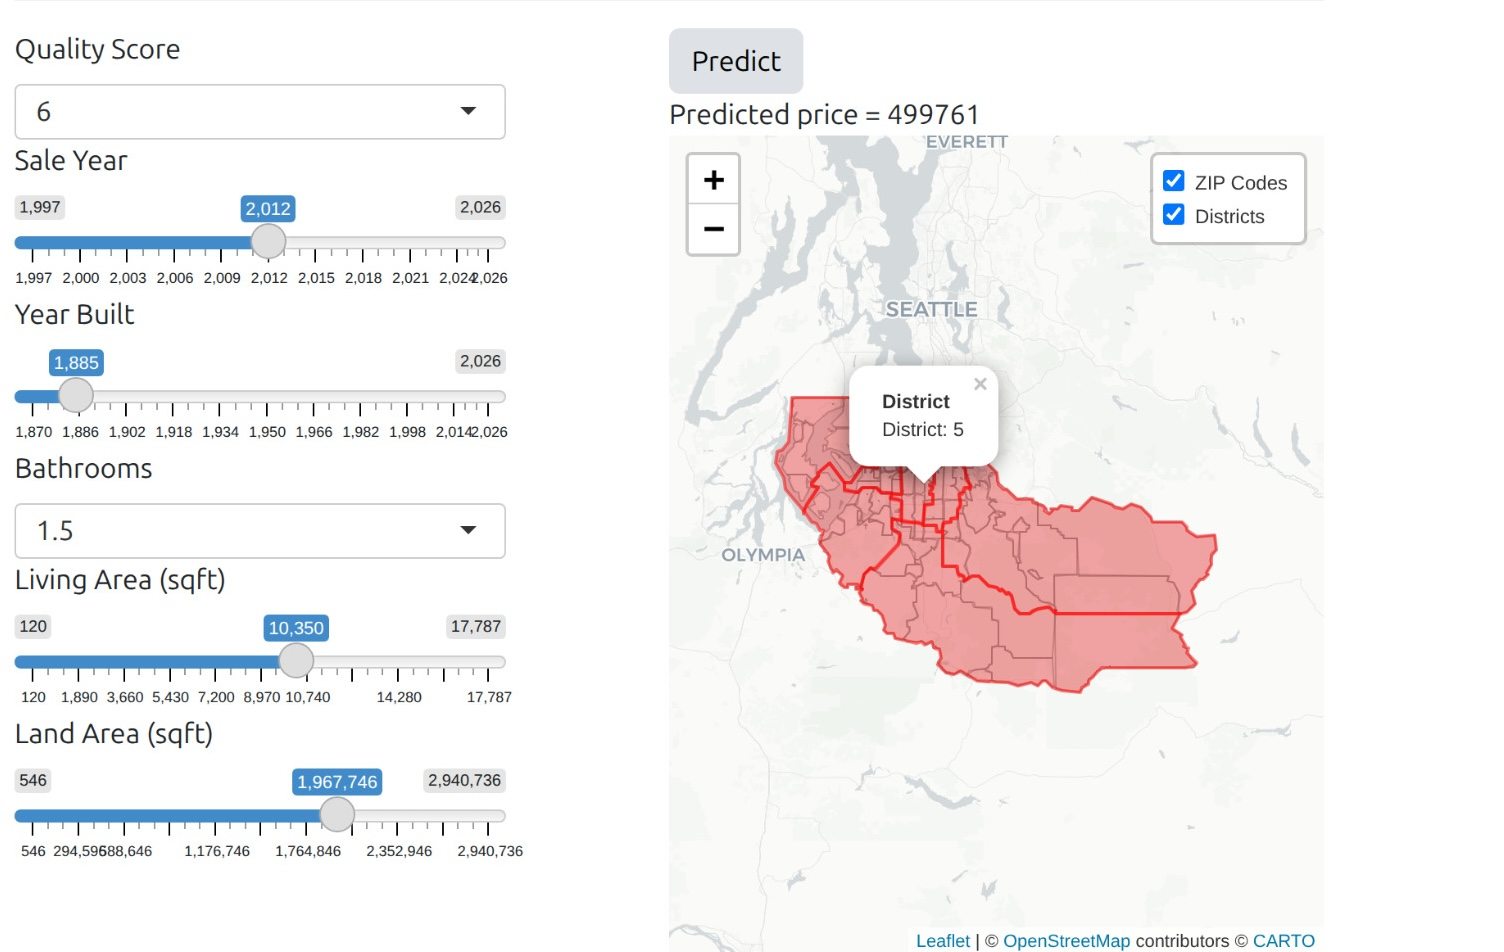
\includegraphics[keepaspectratio]{diagrams/app_demo.jpeg}}

}

\caption{Skeleton of the envisioned app}

\end{figure}%

\cleardoublepage
\phantomsection
\addcontentsline{toc}{part}{Appendices}
\appendix

\chapter{Appendix: Complete Data
Dictionary}\label{appendix-complete-data-dictionary}

\section{Full Field-Level
Definitions}\label{full-field-level-definitions}

This appendix contains the complete field-level data dictionary for all
nine tables in the Pierce County Assessor-Treasurer Data Mart. These
detailed descriptions should be consulted as reference during data
integration, feature engineering, and validation.

\textbf{Source}: Pierce County Assessor-Treasurer Office
https://online.co.pierce.wa.us/cfapps/atr/datamart/metadata/

\begin{center}\rule{0.5\linewidth}{0.5pt}\end{center}

\section{Tax Account}\label{tax-account-1}

Comprehensive tax and assessment account information for each property.

\begin{longtable}[]{@{}
  >{\raggedright\arraybackslash}p{(\linewidth - 6\tabcolsep) * \real{0.2738}}
  >{\raggedright\arraybackslash}p{(\linewidth - 6\tabcolsep) * \real{0.1071}}
  >{\raggedright\arraybackslash}p{(\linewidth - 6\tabcolsep) * \real{0.1071}}
  >{\raggedright\arraybackslash}p{(\linewidth - 6\tabcolsep) * \real{0.5119}}@{}}
\caption{Tax Account table - tax and assessment account
information.}\label{tbl-app-tax-account}\tabularnewline
\toprule\noalign{}
\begin{minipage}[b]{\linewidth}\raggedright
Field Name
\end{minipage} & \begin{minipage}[b]{\linewidth}\raggedright
Type
\end{minipage} & \begin{minipage}[b]{\linewidth}\raggedright
Size
\end{minipage} & \begin{minipage}[b]{\linewidth}\raggedright
Description
\end{minipage} \\
\midrule\noalign{}
\endfirsthead
\toprule\noalign{}
\begin{minipage}[b]{\linewidth}\raggedright
Field Name
\end{minipage} & \begin{minipage}[b]{\linewidth}\raggedright
Type
\end{minipage} & \begin{minipage}[b]{\linewidth}\raggedright
Size
\end{minipage} & \begin{minipage}[b]{\linewidth}\raggedright
Description
\end{minipage} \\
\midrule\noalign{}
\endhead
\bottomrule\noalign{}
\endlastfoot
\textbf{Parcel Number} & Text & 10 & Unique 10 digit number assigned to
each property \\
Account Type & Text & 5 & REAL - Real Property; STRUC - Structures; PERS
- Personal Property; MOBIL - Mobile Home \\
Property Type & Text & 5 & ASIMP - Administrative Seg Improvement; LNDIM
- Land and Improvements; MBLHM - Mobile Home; RRLEA - Railroad Leases;
SAPP - State Assessed Personal Property; SARP - State Assessed Real
Property; STRUC - Leased Land and/or Structure \\
Site Address & Text & 50 & Physical location address of the property.
May be different than mailing address. ``XXX'' indicates estimated
address using GIS \\
Use Code & Text & 5 & 4-digit numeric code for present highest and best
use of the property \\
Use Description & Text & 50 & Text description of the numeric use
code \\
Tax Year - Prior & Integer & & Tax year for which all prior year values
apply \\
Tax Code Area - Prior Year & Text & 10 & Code describing geographical
area and specific combination of taxing districts. Subject to annual
change \\
Exemption Type - Prior Year & Text & 40 & Type of exemption, if any,
applied to the property \\
Current Use Code - Prior Year & Text & 5 & AGRI - Agricultural; CT -
Current Use Timber; FORDG - Forest Designated; OPBRS - Open Space PBRS;
OPEN - Open Space \\
Land Value - Prior Year & Integer & & Total fair market value of land,
as determined by appraisal process \\
Improvement Value - Prior Year & Integer & & Total fair market value of
improvements (buildings, structures), as determined by appraisal
process \\
Total Market Value - Prior Year & Integer & & Total fair market value of
land and improvements, as determined by appraisal process \\
Taxable Value - Prior Year & Integer & & Market value of the property,
minus any exemptions granted \\
Tax Year - Current & Integer & & Tax year for which all current year
values apply \\
Tax Code Area - Current Year & Text & 10 & Code describing geographical
area and specific combination of taxing districts \\
Exemption Type - Current Year & Text & 40 & Type of exemption, if any,
applied to the property \\
Current Use Code - Current Year & Text & 5 & AGRI - Agricultural; CT -
Current Use Timber; FORDG - Forest Designated; OPBRS - Open Space PBRS;
OPEN - Open Space \\
Land Value - Current Year & Integer & & Total fair market value of land
for the parcel \\
Improvement Value - Current Year & Integer & & Total fair market value
of improvements (buildings, structures) for the parcel \\
Total Market Value - Current Year & Integer & & Total fair market value
of land and improvements for the parcel \\
Taxable Value - Current Year & Integer & & Market value of the property,
minus any exemptions granted \\
Range & Text & 10 & Range \\
Township & Text & 10 & Township \\
Section & Text & 20 & Section \\
Quarter Section & Text & 20 & Quarter \\
Subdivision Name & Text & 50 & Subdivision name \\
Located On Parcel & Text & 10 & Real property parcel number on which
this improvement-only parcel is located (Personal Property, Mobile
Homes, Leasehold Structures) \\
\end{longtable}

\begin{center}\rule{0.5\linewidth}{0.5pt}\end{center}

\section{Appraisal Account}\label{appraisal-account-1}

Detailed property appraisal data with characteristics and valuations.

\begin{longtable}[]{@{}
  >{\raggedright\arraybackslash}p{(\linewidth - 6\tabcolsep) * \real{0.2738}}
  >{\raggedright\arraybackslash}p{(\linewidth - 6\tabcolsep) * \real{0.1071}}
  >{\raggedright\arraybackslash}p{(\linewidth - 6\tabcolsep) * \real{0.1071}}
  >{\raggedright\arraybackslash}p{(\linewidth - 6\tabcolsep) * \real{0.5119}}@{}}
\caption{Appraisal Account table - property appraisal data with
characteristics.}\label{tbl-app-appraisal-account}\tabularnewline
\toprule\noalign{}
\begin{minipage}[b]{\linewidth}\raggedright
Field Name
\end{minipage} & \begin{minipage}[b]{\linewidth}\raggedright
Type
\end{minipage} & \begin{minipage}[b]{\linewidth}\raggedright
Size
\end{minipage} & \begin{minipage}[b]{\linewidth}\raggedright
Description
\end{minipage} \\
\midrule\noalign{}
\endfirsthead
\toprule\noalign{}
\begin{minipage}[b]{\linewidth}\raggedright
Field Name
\end{minipage} & \begin{minipage}[b]{\linewidth}\raggedright
Type
\end{minipage} & \begin{minipage}[b]{\linewidth}\raggedright
Size
\end{minipage} & \begin{minipage}[b]{\linewidth}\raggedright
Description
\end{minipage} \\
\midrule\noalign{}
\endhead
\bottomrule\noalign{}
\endlastfoot
\textbf{Parcel Number} & Text & 10 & Unique 10 digit number assigned to
each property \\
Appraisal Account Type & Text & 15 & Com Condo, Com Leasehold, Com Multi
Unit, Commercial, Industrial, Mobile Home, Reference, Res Com Condo, Res
Leasehold, Residential, Trended Invest \\
Business Name & Text & 50 & Main business name on the parcel, or space
number for mobile/manufactured home in a park \\
Value Area ID & Text & 10 & Identifies the Physical Inspection cycle for
each parcel (PI1 to PI6) \\
Land Economic Area & Text & 30 & Ties parcels to land valuation models;
identifies land use model by PI year or appraisal
area/sector/subsector \\
Buildings & Integer & & Represents the number of improvements
(buildings) located on a parcel \\
Group Account Number & Text & 30 & Identifies all parcels as one
economic unit or condominium project \\
Land Gross Acres & Decimal & 15.4 & Total acres that make up the
economic unit which could include multiple parcels \\
Land Net Acres & Decimal & 15.4 & Size of the individual parcel in
acres \\
Land Gross Square Feet & Decimal & 15.4 & Total square feet that make up
the economic unit which could include multiple parcels \\
Land Net Square Feet & Decimal & 15.4 & Size of the individual parcel in
square feet \\
Land Gross Front Feet & Decimal & 15.4 & Front feet of site facing
arterial (commercial), address side (residential), or waterfront
length \\
Land Width & Integer & & Net Effective Waterfront Front Feet of
individual parcel (Residential Use Only) \\
Land Depth & Integer & & Net Effective Depth from top of bank to inland
property line (Residential Use Only) \\
Submerged Area Square Feet & Integer & & Area of a parcel that is
submerged; not included in Gross or Net Square Feet \\
Appraisal Date & Date & & Most recent date an appraiser physically
observed the property and/or made changes \\
Waterfront Type & Text & 30 & Describes the type of waterfront the
property adjoins or has legal access to \\
View Quality & Text & 30 & Market appeal rating of overall view
available from dwelling or property \\
Utility Electric & Text & 30 & Identifies if power is installed,
available, or not available on the property \\
Utility Sewer & Text & 30 & Identifies if sewer/septic is installed,
available, or not available \\
Utility Water & Text & 30 & Identifies if water is installed, available,
or not available \\
Street Type & Text & 30 & Identifies if access street is paved or
unpaved \\
Latitude & Decimal & 10.5 & Latitude of parcel centroid (some parcels
may not have coordinates) \\
Longitude & Decimal & 10.5 & Longitude of parcel centroid \\
\end{longtable}

\begin{center}\rule{0.5\linewidth}{0.5pt}\end{center}

\section{Improvement}\label{improvement-1}

Detailed building improvement data linked to appraisal accounts.

\begin{longtable}[]{@{}
  >{\raggedright\arraybackslash}p{(\linewidth - 6\tabcolsep) * \real{0.2738}}
  >{\raggedright\arraybackslash}p{(\linewidth - 6\tabcolsep) * \real{0.1071}}
  >{\raggedright\arraybackslash}p{(\linewidth - 6\tabcolsep) * \real{0.1071}}
  >{\raggedright\arraybackslash}p{(\linewidth - 6\tabcolsep) * \real{0.5119}}@{}}
\caption{Improvement table - building improvement data linked to
appraisal accounts.}\label{tbl-app-improvement}\tabularnewline
\toprule\noalign{}
\begin{minipage}[b]{\linewidth}\raggedright
Field Name
\end{minipage} & \begin{minipage}[b]{\linewidth}\raggedright
Type
\end{minipage} & \begin{minipage}[b]{\linewidth}\raggedright
Size
\end{minipage} & \begin{minipage}[b]{\linewidth}\raggedright
Description
\end{minipage} \\
\midrule\noalign{}
\endfirsthead
\toprule\noalign{}
\begin{minipage}[b]{\linewidth}\raggedright
Field Name
\end{minipage} & \begin{minipage}[b]{\linewidth}\raggedright
Type
\end{minipage} & \begin{minipage}[b]{\linewidth}\raggedright
Size
\end{minipage} & \begin{minipage}[b]{\linewidth}\raggedright
Description
\end{minipage} \\
\midrule\noalign{}
\endhead
\bottomrule\noalign{}
\endlastfoot
\textbf{Parcel Number} & Text & 10 & Unique 10 digit number assigned to
each property \\
\textbf{Building ID} & Text & 5 & Unique identifier for each improvement
record on a parcel \\
Property Type & Text & 15 & Links buildings to cost and depreciation
tables: Commercial, Duplex, Industrial, Mobile Home, Multiple Unit, Out
Building, Residential, Townhouse, Triplex \\
Neighborhood & Text & 10 & Boundaries for land subject to similar
social, environmental, economic, and governmental forces \\
Neighborhood Extension & Text & 10 & Based on property type: primary
occupancy (Commercial), zero (Residential), or park designation (Mobile
Homes) \\
Square Feet & Integer & & Sum of square feet for `built as' types (may
represent count for Storage Tank types) \\
Net Square Feet & Integer & & Sum of net rentable area(s) for
commercial; equal to built-as square feet or zero for residential \\
\end{longtable}

\begin{center}\rule{0.5\linewidth}{0.5pt}\end{center}

\section{Improvement Built-As}\label{improvement-built-as-1}

Detailed specifications for building construction styles and features.

\begin{longtable}[]{@{}
  >{\raggedright\arraybackslash}p{(\linewidth - 6\tabcolsep) * \real{0.2738}}
  >{\raggedright\arraybackslash}p{(\linewidth - 6\tabcolsep) * \real{0.1071}}
  >{\raggedright\arraybackslash}p{(\linewidth - 6\tabcolsep) * \real{0.1071}}
  >{\raggedright\arraybackslash}p{(\linewidth - 6\tabcolsep) * \real{0.5119}}@{}}
\caption{Improvement Built-As table - building construction styles and
features.}\label{tbl-app-builtas}\tabularnewline
\toprule\noalign{}
\begin{minipage}[b]{\linewidth}\raggedright
Field Name
\end{minipage} & \begin{minipage}[b]{\linewidth}\raggedright
Type
\end{minipage} & \begin{minipage}[b]{\linewidth}\raggedright
Size
\end{minipage} & \begin{minipage}[b]{\linewidth}\raggedright
Description
\end{minipage} \\
\midrule\noalign{}
\endfirsthead
\toprule\noalign{}
\begin{minipage}[b]{\linewidth}\raggedright
Field Name
\end{minipage} & \begin{minipage}[b]{\linewidth}\raggedright
Type
\end{minipage} & \begin{minipage}[b]{\linewidth}\raggedright
Size
\end{minipage} & \begin{minipage}[b]{\linewidth}\raggedright
Description
\end{minipage} \\
\midrule\noalign{}
\endhead
\bottomrule\noalign{}
\endlastfoot
\textbf{Parcel Number} & Text & 10 & Unique 10 digit number assigned to
each property \\
\textbf{Building ID} & Text & 5 & Unique identifier for each improvement
record on a parcel \\
\textbf{Built-As Number} & Integer & & Sequential number starting with
largest Built-As being number 1 \\
Built-As ID & Integer & & Number associated with the description of the
purpose or style of construction \\
Built-As Description & Text & 255 & Original purpose/style of
construction; associated with Marshall and Swift cost and depreciation
tables \\
Built-As Square Feet & Integer & & Sum of square feet for the `built as'
types identified for the building \\
HVAC & Integer & & Code associated with the predominant heating source
for the built-as structure \\
HVAC Description & Text & 30 & Text description of heating source
(Forced Air, Electric Baseboard, Steam, etc) \\
Exterior & Text & 25 & Predominant type of construction materials used
for exterior siding (Residential Buildings) \\
Interior & Text & 15 & Predominant type of interior wall materials
(Sheetrock or Paneling; Residential and Mobile Homes only) \\
Stories & Decimal & 13.2 & Number of floors/building levels above grade
(excluding attic or basement) \\
Story Height & Integer & & Average ceiling heights (Commercial) or
majority story height for first floor (Residential) \\
Sprinkler Square Feet & Integer & & Total square footage covered by a
sprinkler system \\
Roof Cover & Text & 20 & Material used for the roof (Composition
Shingles, Wood Shake, Concrete Tile, etc) \\
Bedrooms & Integer & & Number of bedrooms listed for residential
property \\
Bathrooms & Decimal & 7.2 & Number of baths listed as decimal (e.g.,
2.75 = two full + one three-quarter) \\
Units & Integer & & Number of separate units within the building \\
Class Code & Text & 20 & Code for one of five basic cost groups by type
of framing, walls, floors, roof, and fireproofing \\
Class Description & Text & 50 & Text description for cost group
classification \\
Year Built & Integer & & Year the building was built per building permit
or historical record \\
Year Remodeled & Integer & & Year improvements were made extending the
life of the structure \\
Adjusted Year Built & Integer & & Greater than Year Built if
improvements reduce the effective age of the building \\
Physical Age & Integer & & Tax year less adjusted year built \\
Built-As Length & Integer & & Length of the mobile/manufactured home \\
Built-As Width & Integer & & Width of the mobile/manufactured home \\
Mobile Home Model & Text & 50 & Model of the mobile/manufactured home \\
\end{longtable}

\begin{center}\rule{0.5\linewidth}{0.5pt}\end{center}

\section{Improvement Detail}\label{improvement-detail-1}

Additional specific improvement characteristics and features.

\begin{longtable}[]{@{}
  >{\raggedright\arraybackslash}p{(\linewidth - 6\tabcolsep) * \real{0.2738}}
  >{\raggedright\arraybackslash}p{(\linewidth - 6\tabcolsep) * \real{0.1071}}
  >{\raggedright\arraybackslash}p{(\linewidth - 6\tabcolsep) * \real{0.1071}}
  >{\raggedright\arraybackslash}p{(\linewidth - 6\tabcolsep) * \real{0.5119}}@{}}
\caption{Improvement Detail table - building characteristics and
features.}\label{tbl-app-detail}\tabularnewline
\toprule\noalign{}
\begin{minipage}[b]{\linewidth}\raggedright
Field Name
\end{minipage} & \begin{minipage}[b]{\linewidth}\raggedright
Type
\end{minipage} & \begin{minipage}[b]{\linewidth}\raggedright
Size
\end{minipage} & \begin{minipage}[b]{\linewidth}\raggedright
Description
\end{minipage} \\
\midrule\noalign{}
\endfirsthead
\toprule\noalign{}
\begin{minipage}[b]{\linewidth}\raggedright
Field Name
\end{minipage} & \begin{minipage}[b]{\linewidth}\raggedright
Type
\end{minipage} & \begin{minipage}[b]{\linewidth}\raggedright
Size
\end{minipage} & \begin{minipage}[b]{\linewidth}\raggedright
Description
\end{minipage} \\
\midrule\noalign{}
\endhead
\bottomrule\noalign{}
\endlastfoot
\textbf{Parcel Number} & Text & 10 & Unique 10 digit number assigned to
each property \\
\textbf{Building ID} & Text & 5 & Unique identifier for each improvement
record on a parcel \\
\textbf{Detail Type} & Text & 10 & Category: Add On, Appliance, Balcony,
Basement, Carport, Elevator, Fixture, Garage, Mezzanine, Porch, Rough
In, Storage \\
Detail Description & Text & 50 & Brief explanation of the improvement
characteristic (Fireplace, Laundry Facility, Type of Porch, Type of
Bath, etc) \\
Units & Decimal & 15.4 & Component parts indicating either square
footage of the structure or count of each component \\
\end{longtable}

\begin{center}\rule{0.5\linewidth}{0.5pt}\end{center}

\section{Land Attribute}\label{land-attribute-1}

Land-specific attributes and characteristics affecting valuation.

\begin{longtable}[]{@{}
  >{\raggedright\arraybackslash}p{(\linewidth - 6\tabcolsep) * \real{0.2738}}
  >{\raggedright\arraybackslash}p{(\linewidth - 6\tabcolsep) * \real{0.1071}}
  >{\raggedright\arraybackslash}p{(\linewidth - 6\tabcolsep) * \real{0.1071}}
  >{\raggedright\arraybackslash}p{(\linewidth - 6\tabcolsep) * \real{0.5119}}@{}}
\caption{Land Attribute table - land-specific characteristics affecting
valuation.}\label{tbl-app-land}\tabularnewline
\toprule\noalign{}
\begin{minipage}[b]{\linewidth}\raggedright
Field Name
\end{minipage} & \begin{minipage}[b]{\linewidth}\raggedright
Type
\end{minipage} & \begin{minipage}[b]{\linewidth}\raggedright
Size
\end{minipage} & \begin{minipage}[b]{\linewidth}\raggedright
Description
\end{minipage} \\
\midrule\noalign{}
\endfirsthead
\toprule\noalign{}
\begin{minipage}[b]{\linewidth}\raggedright
Field Name
\end{minipage} & \begin{minipage}[b]{\linewidth}\raggedright
Type
\end{minipage} & \begin{minipage}[b]{\linewidth}\raggedright
Size
\end{minipage} & \begin{minipage}[b]{\linewidth}\raggedright
Description
\end{minipage} \\
\midrule\noalign{}
\endhead
\bottomrule\noalign{}
\endlastfoot
\textbf{Parcel Number} & Text & 10 & Unique 10 digit number assigned to
each property \\
\textbf{Attribute} & Text & 30 & Category: Residential (R), Commercial
(C), or Res Com Condo (X) with subcategory \\
Attribute Description & Text & 30 & Further defines the land attribute
(View Avg, NBHD Gated, WF Bank Low, water available, etc) \\
\end{longtable}

\begin{center}\rule{0.5\linewidth}{0.5pt}\end{center}

\section{Sale}\label{sale-1}

Historical property sales transaction data.

\begin{longtable}[]{@{}
  >{\raggedright\arraybackslash}p{(\linewidth - 6\tabcolsep) * \real{0.2738}}
  >{\raggedright\arraybackslash}p{(\linewidth - 6\tabcolsep) * \real{0.1071}}
  >{\raggedright\arraybackslash}p{(\linewidth - 6\tabcolsep) * \real{0.1071}}
  >{\raggedright\arraybackslash}p{(\linewidth - 6\tabcolsep) * \real{0.5119}}@{}}
\caption{Sale table - historical property sales transaction
data.}\label{tbl-app-sale}\tabularnewline
\toprule\noalign{}
\begin{minipage}[b]{\linewidth}\raggedright
Field Name
\end{minipage} & \begin{minipage}[b]{\linewidth}\raggedright
Type
\end{minipage} & \begin{minipage}[b]{\linewidth}\raggedright
Size
\end{minipage} & \begin{minipage}[b]{\linewidth}\raggedright
Description
\end{minipage} \\
\midrule\noalign{}
\endfirsthead
\toprule\noalign{}
\begin{minipage}[b]{\linewidth}\raggedright
Field Name
\end{minipage} & \begin{minipage}[b]{\linewidth}\raggedright
Type
\end{minipage} & \begin{minipage}[b]{\linewidth}\raggedright
Size
\end{minipage} & \begin{minipage}[b]{\linewidth}\raggedright
Description
\end{minipage} \\
\midrule\noalign{}
\endhead
\bottomrule\noalign{}
\endlastfoot
\textbf{ETN} & Text & 11 & Recording number issued by the Auditor's
Office when property transaction is recorded \\
Parcel Count & Integer & & Number of parcels associated with a sale \\
Parcel Number & Text & 10 & Unique 10 digit number assigned to each
property \\
Sale Date & Date & & Date the legal document (deed) was executed \\
Sale Price & Decimal & 15.2 & Dollar amount recorded on the ETN \\
Deed Type & Text & 40 & Type of document conveying interest in or legal
title to the property \\
Grantor & Text & 80 & Individual(s) or company conveying ownership or
interest in the property \\
Grantee & Text & 80 & Individual(s) or company purchasing ownership or
interest in the property \\
Valid/Invalid & Text & 7 & Code for validity of a sale for appraisal
purposes per State Ratio RCW \\
Confirmed/Unconfirmed & Text & 11 & Whether property characteristics and
sale circumstances were verified by Assessor-Treasurer staff \\
Exclude Reason & Text & 30 & State required description of why a sales
transaction must be excluded from sales studies \\
Improved/Vacant & Text & 8 & Coded as improved if any parcel has
building value; vacant for land with no building value \\
Appraisal Account Type & Text & 15 & Parcel classification (Com Condo,
Com Leasehold, Commercial, Industrial, Residential, etc) \\
\end{longtable}

\begin{center}\rule{0.5\linewidth}{0.5pt}\end{center}

\section{Seg/Merge}\label{segmerge-1}

Property segregation and merger transaction history.

\begin{longtable}[]{@{}
  >{\raggedright\arraybackslash}p{(\linewidth - 6\tabcolsep) * \real{0.2738}}
  >{\raggedright\arraybackslash}p{(\linewidth - 6\tabcolsep) * \real{0.1071}}
  >{\raggedright\arraybackslash}p{(\linewidth - 6\tabcolsep) * \real{0.1071}}
  >{\raggedright\arraybackslash}p{(\linewidth - 6\tabcolsep) * \real{0.5119}}@{}}
\caption{Seg/Merge table - property segregation and merger transaction
history.}\label{tbl-app-segmerge}\tabularnewline
\toprule\noalign{}
\begin{minipage}[b]{\linewidth}\raggedright
Field Name
\end{minipage} & \begin{minipage}[b]{\linewidth}\raggedright
Type
\end{minipage} & \begin{minipage}[b]{\linewidth}\raggedright
Size
\end{minipage} & \begin{minipage}[b]{\linewidth}\raggedright
Description
\end{minipage} \\
\midrule\noalign{}
\endfirsthead
\toprule\noalign{}
\begin{minipage}[b]{\linewidth}\raggedright
Field Name
\end{minipage} & \begin{minipage}[b]{\linewidth}\raggedright
Type
\end{minipage} & \begin{minipage}[b]{\linewidth}\raggedright
Size
\end{minipage} & \begin{minipage}[b]{\linewidth}\raggedright
Description
\end{minipage} \\
\midrule\noalign{}
\endhead
\bottomrule\noalign{}
\endlastfoot
\textbf{Seg/Merge Number} & Text & 12 & Unique number assigned to each
segregation \\
Parent/Child Indicator & Text & 1 & P = Parent Parcel (inactivated); C =
Child Parcel (newly created from segregation) \\
\textbf{Parcel Number} & Text & 10 & Unique 10 digit number assigned to
each property \\
Continued Indicator & Text & 1 & Y = parcel still active after
segregation; N = parcel no longer active \\
Completed Date & Date & & Date that the segregation was completed \\
Tax Year & Text & 4 & Tax year of the segregation \\
\end{longtable}

\begin{center}\rule{0.5\linewidth}{0.5pt}\end{center}

\section{Taxpayer}\label{taxpayer-1}

Property owner information (subject to privacy restrictions).

\begin{longtable}[]{@{}
  >{\raggedright\arraybackslash}p{(\linewidth - 6\tabcolsep) * \real{0.2738}}
  >{\raggedright\arraybackslash}p{(\linewidth - 6\tabcolsep) * \real{0.1071}}
  >{\raggedright\arraybackslash}p{(\linewidth - 6\tabcolsep) * \real{0.1071}}
  >{\raggedright\arraybackslash}p{(\linewidth - 6\tabcolsep) * \real{0.5119}}@{}}
\caption{Taxpayer table - property owner information (privacy
restricted).}\label{tbl-app-taxpayer}\tabularnewline
\toprule\noalign{}
\begin{minipage}[b]{\linewidth}\raggedright
Field Name
\end{minipage} & \begin{minipage}[b]{\linewidth}\raggedright
Type
\end{minipage} & \begin{minipage}[b]{\linewidth}\raggedright
Size
\end{minipage} & \begin{minipage}[b]{\linewidth}\raggedright
Description
\end{minipage} \\
\midrule\noalign{}
\endfirsthead
\toprule\noalign{}
\begin{minipage}[b]{\linewidth}\raggedright
Field Name
\end{minipage} & \begin{minipage}[b]{\linewidth}\raggedright
Type
\end{minipage} & \begin{minipage}[b]{\linewidth}\raggedright
Size
\end{minipage} & \begin{minipage}[b]{\linewidth}\raggedright
Description
\end{minipage} \\
\midrule\noalign{}
\endhead
\bottomrule\noalign{}
\endlastfoot
\textbf{Parcel Number} & Text & 10 & Unique 10 digit number assigned to
each property \\
\end{longtable}

\begin{center}\rule{0.5\linewidth}{0.5pt}\end{center}

\section{Tax Description}\label{tax-description-1}

Detailed tax coding and descriptions for parcels.

\begin{longtable}[]{@{}
  >{\raggedright\arraybackslash}p{(\linewidth - 6\tabcolsep) * \real{0.2738}}
  >{\raggedright\arraybackslash}p{(\linewidth - 6\tabcolsep) * \real{0.1071}}
  >{\raggedright\arraybackslash}p{(\linewidth - 6\tabcolsep) * \real{0.1071}}
  >{\raggedright\arraybackslash}p{(\linewidth - 6\tabcolsep) * \real{0.5119}}@{}}
\caption{Tax Description table - tax coding and descriptions for
parcels.}\label{tbl-app-tax-description}\tabularnewline
\toprule\noalign{}
\begin{minipage}[b]{\linewidth}\raggedright
Field Name
\end{minipage} & \begin{minipage}[b]{\linewidth}\raggedright
Type
\end{minipage} & \begin{minipage}[b]{\linewidth}\raggedright
Size
\end{minipage} & \begin{minipage}[b]{\linewidth}\raggedright
Description
\end{minipage} \\
\midrule\noalign{}
\endfirsthead
\toprule\noalign{}
\begin{minipage}[b]{\linewidth}\raggedright
Field Name
\end{minipage} & \begin{minipage}[b]{\linewidth}\raggedright
Type
\end{minipage} & \begin{minipage}[b]{\linewidth}\raggedright
Size
\end{minipage} & \begin{minipage}[b]{\linewidth}\raggedright
Description
\end{minipage} \\
\midrule\noalign{}
\endhead
\bottomrule\noalign{}
\endlastfoot
\textbf{Parcel Number} & Text & 10 & Unique 10 digit number assigned to
each property \\
\textbf{Line Number} & Integer & & Sequential number identifying each
line of a tax description \\
Tax Description Line & Text & 200 & Tax description text \\
\end{longtable}




\end{document}
